\documentclass[11pt,a4paper]{article}
\usepackage[utf8]{inputenc}
\usepackage{amsmath,amssymb,amsfonts}
\usepackage{geometry}
\usepackage{booktabs}
\usepackage{array}
\usepackage{longtable}
\usepackage{graphicx}
\usepackage{listings}
\usepackage{xcolor}

% Global listings settings for better text fitting
\lstset{
    breaklines=true,
    breakatwhitespace=true,
    postbreak=\mbox{\textcolor{red}{$\hookrightarrow$}\space},
    columns=flexible
}

% Allow more flexible line breaking to prevent overfull boxes
\tolerance=1000
\emergencystretch=3em
\hyphenpenalty=500
\usepackage{hyperref}
\usepackage{algorithm}
\usepackage{algpseudocode}
\usepackage{tikz}
\usetikzlibrary{shapes.geometric, arrows.meta, positioning, fit, backgrounds, calc, decorations.pathreplacing}
\usepackage[most]{tcolorbox}
\usepackage{fancyhdr}
\usepackage{enumitem}

\geometry{margin=1in}

% Page style with footer
\pagestyle{fancy}
\fancyhf{}
\fancyhead[L]{\leftmark}
\fancyhead[R]{\thepage}
\fancyfoot[L]{\textcopyright\ Space Labs AI}
\fancyfoot[C]{Space-Radiation-Tolerant}
\fancyfoot[R]{AGPL-3.0 License}
\renewcommand{\headrulewidth}{0.4pt}
\renewcommand{\footrulewidth}{0.4pt}

% Apply fancy style to plain pages (like title page, ToC)
\fancypagestyle{plain}{
    \fancyhf{}
    \fancyfoot[L]{\textcopyright\ Space Labs AI}
    \fancyfoot[C]{Space-Radiation-Tolerant}
    \fancyfoot[R]{AGPL-3.0 License}
    \renewcommand{\headrulewidth}{0pt}
    \renewcommand{\footrulewidth}{0.4pt}
}

% TikZ styles for architecture diagrams
\tikzset{
  module/.style={rectangle, rounded corners, minimum width=2.5cm, minimum height=1cm, text centered, draw=black, fill=blue!20, font=\small},
  submodule/.style={rectangle, rounded corners, minimum width=2cm, minimum height=0.7cm, text centered, draw=black, fill=green!20, font=\footnotesize},
  process/.style={rectangle, minimum width=2cm, minimum height=0.8cm, text centered, draw=black, fill=orange!20, font=\small},
  decision/.style={diamond, aspect=2, minimum width=1.5cm, minimum height=0.8cm, text centered, draw=black, fill=yellow!20, font=\footnotesize},
  data/.style={trapezium, trapezium left angle=70, trapezium right angle=110, minimum width=1.5cm, minimum height=0.6cm, text centered, draw=black, fill=gray!20, font=\small},
  arrow/.style={thick,->,>=stealth},
  dashedarrow/.style={thick,->,>=stealth,dashed},
  brace/.style={decorate, decoration={brace, amplitude=5pt, raise=2pt}}
}

\title{\textbf{RadML: Complete Manual for } \\
Radiation-Tolerant Machine Learning Framework}
\author{Rishab Nuguru \\ \textit{Space Labs AI}}
\date{\today}

\begin{document}

\maketitle

\vspace{1em}
\begin{center}
\fbox{\parbox{0.85\textwidth}{
\centering\textit{``The core of sustainability is building for the next generation.''}
}}
\end{center}
\vspace{1em}

\begin{abstract}
\noindent
Deployment of commercial off-the-shelf (COTS) AI accelerators in deep space is currently limited by their susceptibility to single-event effects (SEE), particularly in deep-nanometer ($<7\text{nm}$) process nodes where quantum tunneling and confinement effects invalidate classical error rate models. Existing mitigation strategies rely on either computationally expensive offline Monte Carlo simulations (e.g., Geant4) or reactive, static redundancy (e.g., Triple Modular Redundancy), which imposes fixed overheads regardless of environmental severity.

Space Labs AI's manual documents \textbf{RadML}, a \textbf{software-defined approach} to radiation tolerance that embeds a physics engine directly into flight software. Designed to work \textit{alongside} traditional radiation-hardened (rad-hard) components and physical shielding, RadML provides an additional layer of protection through intelligent, adaptive fault tolerance. By treating software protection as a dynamic resource allocated according to real-time physical risk, RadML enables the confident utilization of high-performance COTS hardware in hybrid rad-hard architectures.

\vspace{0.5em}
\noindent\textbf{Core Innovations:}
\begin{itemize}
    \item \textbf{Quantum-Corrected SEU Model:} Augments empirical Weibull/Bendel cross-section fits with real-time solutions to the Dirac and Bethe-Salpeter equations, correcting Linear Energy Transfer (LET) calculations for quantum tunneling probabilities in nanoscale transistors.
    \item \textbf{Closed-Loop Adaptive Protection:} Ingests orbital telemetry (particle flux, solar modulation, SAA position) to dynamically scale error correction schemes---shifting from low-overhead Parity checks in quiet regimes to Reed-Solomon (RS-16) coding during Solar Particle Events (SPE).
    \item \textbf{Zero-Overhead Abstractions:} Shifts the computational burden of error correction from runtime execution to compile-time template metaprogramming, achieving near-native performance while providing defense-in-depth reliability.
\end{itemize}

\vspace{0.5em}
\noindent\textbf{Application:} RadML is designed as a \textbf{complementary layer} within hybrid radiation hardening strategies---not a replacement for physical shielding or rad-hard components, but a software-defined enhancement that provides additional safety margins. By layering adaptive, physics-aware fault tolerance atop traditional protection methods, RadML enables mission architects to confidently deploy COTS components in Geostationary Orbit (GEO), Lunar, and interplanetary missions while maintaining the reliability standards required for autonomous deep-space AI systems.

\vspace{0.5em}
\noindent\textbf{Keywords:} Software-Defined Radiation Tolerance, Radiation Hardening by Software (RHBS), Hybrid Rad-Hard Architectures, Quantum-Corrected SEU, Adaptive Fault Tolerance, COTS in Space, Defense-in-Depth.
\end{abstract}

\tableofcontents
\newpage

\section{Fundamental Physics}

\begin{tcolorbox}[colback=blue!5!white,colframe=blue!75!black,title=Physics Model Integration,breakable]
\textbf{RadML uses a hybrid approach}: validated engineering models for production SEU rates, with quantum corrections for improved accuracy.

\vspace{0.3em}
\textbf{Production Layer:} (\texttt{physics/radiation\_physics.hpp})
\begin{itemize}[noitemsep,topsep=0pt]
    \item \textbf{Weibull/Bendel} cross-sections -- Calibrated to ground test data
    \item \textbf{Radiation flux models} -- Adams GCR (LET-based), AP-8-inspired trapped protons, AE-8-inspired trapped electrons, SAA
\end{itemize}

\textbf{Correction Layer:} (\texttt{quantum\_enhanced\_radiation.hpp})
\begin{itemize}[noitemsep,topsep=0pt]
    \item Quantum corrections via \texttt{applyQuantumFieldCorrections()} (free function in \texttt{quantum\_field\_theory.hpp})
    \item Device sensitivity: SRAM 1.0$\times$, DRAM 1.5$\times$, MRAM 0.1$\times$
\end{itemize}

\textbf{Research Layer:} (\texttt{quantum\_field\_theory.hpp})
\begin{itemize}[noitemsep,topsep=0pt]
    \item Dirac, Bethe-Salpeter, Green's Functions -- for validation
\end{itemize}

\textbf{Transport Foundation:} (\texttt{transport\_equation.hpp})
\begin{itemize}[noitemsep,topsep=0pt]
    \item NASA flux = pre-computed transport solutions
    \item SEU Rate = $\int \Phi(E) \cdot \sigma(E) \, dE$
\end{itemize}

\textbf{Summary:} Engineering models $\to$ Base SEU rate. Quantum models $\to$ Correction factors. Both implemented; quantum layer is optional.
\end{tcolorbox}

\subsection{Single Event Upset (SEU) Rate Calculation}

\subsubsection{Master Equation}

The fundamental SEU rate is computed by integrating the particle flux spectrum with the device cross-section:

\begin{equation}
R_{\text{SEU}} = \int_0^\infty \Phi(E) \cdot \sigma(E) \, dE
\end{equation}

\begin{table}[htbp]
\centering
\caption{SEU Rate Equation Field Definitions}
\begin{tabular}{@{}llll@{}}
\toprule
\textbf{Symbol} & \textbf{Name} & \textbf{Units} & \textbf{Typical Values} \\ \midrule
$R_{\text{SEU}}$ & SEU Rate & errors/bit/day & $10^{-5}$ to $10^{-3}$ \\
$\Phi(E)$ & Differential Flux & particles/(cm$^2\cdot$s$\cdot$MeV) & Varies by orbit \\
$\sigma(E)$ & Cross-section & cm$^2$/bit & $10^{-14}$ to $10^{-8}$ \\
$E$ & Particle Energy & MeV & 1--10,000 \\ \bottomrule
\end{tabular}
\end{table}

\textbf{Physical Logic:}
\begin{equation}
\boxed{\text{Upset Rate} = \text{(Particles arriving)} \times \text{(Upset probability per particle)}}
\end{equation}

\subsubsection{Integration Explained}

The integral sums over all energies from 0 to infinity. At each energy $E$:
\begin{itemize}
    \item Count particles arriving: $\Phi(E)$
    \item Multiply by upset chance: $\sigma(E)$
    \item Add to total rate
\end{itemize}

Numerical integration using trapezoidal rule:
\begin{equation}
\int_a^b f(E) \, dE \approx \sum_{i=1}^{N} \frac{f(E_i) + f(E_{i+1})}{2} \cdot (E_{i+1} - E_i)
\end{equation}

\subsection{Weibull Cross-Section Model (Heavy Ions)}

\subsubsection{Formula}

For heavy ions striking silicon, the SEU cross-section as a function of Linear Energy Transfer (LET) follows:

\begin{equation}
\sigma(L) = \begin{cases}
\sigma_{\text{sat}} \cdot \left[1 - \exp\left(-\left(\frac{L - L_{\text{th}}}{W}\right)^s\right)\right] & \text{if } L > L_{\text{th}} \\
0 & \text{if } L \leq L_{\text{th}}
\end{cases}
\end{equation}

\begin{table}[htbp]
\centering
\caption{Weibull Model Parameters}
\begin{tabular}{@{}lllr@{}}
\toprule
\textbf{Symbol} & \textbf{Name} & \textbf{Units} & \textbf{Typical (65nm)} \\ \midrule
$\sigma(L)$ & SEU Cross-section & cm$^2$/bit & $10^{-14}$ to $10^{-8}$ \\
$\sigma_{\text{sat}}$ & Saturation cross-section & cm$^2$/bit & $10^{-8}$ \\
$L$ & Linear Energy Transfer & MeV$\cdot$cm$^2$/mg & 0.1--100 \\
$L_{\text{th}}$ & LET Threshold & MeV$\cdot$cm$^2$/mg & 0.5 \\
$W$ & Weibull Width & MeV$\cdot$cm$^2$/mg & 1--10 \\
$s$ & Weibull Shape & dimensionless & 1--4 \\ \bottomrule
\end{tabular}
\end{table}

\subsubsection{Physical Logic}

\begin{enumerate}
    \item \textbf{Threshold behavior:}
    \begin{equation}
    L < L_{\text{th}} \implies \sigma = 0 \quad \text{(particle too weak)}
    \end{equation}

    \item \textbf{Exponential rise:}
    \begin{equation}
    L \gg L_{\text{th}} \implies \sigma \to \sigma_{\text{sat}} \quad \text{(maximum probability)}
    \end{equation}

    \item \textbf{Transition region:} Shape controlled by $W$ and $s$
\end{enumerate}

\subsubsection{Calculation Example}

Given: $\sigma_{\text{sat}} = 10^{-8}$, $L_{\text{th}} = 0.5$, $W = 3.0$, $s = 2$, $L = 5.0$

\begin{align}
\text{Step 1: } & (L - L_{\text{th}}) = 5.0 - 0.5 = 4.5 \\
\text{Step 2: } & \frac{L - L_{\text{th}}}{W} = \frac{4.5}{3.0} = 1.5 \\
\text{Step 3: } & \left(\frac{L - L_{\text{th}}}{W}\right)^s = (1.5)^2 = 2.25 \\
\text{Step 4: } & \exp(-2.25) = 0.1054 \\
\text{Step 5: } & 1 - 0.1054 = 0.8946 \\
\text{Step 6: } & \sigma(5.0) = 10^{-8} \times 0.8946 = 8.946 \times 10^{-9} \text{ cm}^2/\text{bit}
\end{align}

\subsection{Bendel Proton Model}

\subsubsection{Formula}

Protons cause SEUs through nuclear reactions, not direct ionization:

\begin{equation}
\sigma_p(E) = \begin{cases}
\sigma_\infty \cdot \left[1 - \exp\left(-0.18\left(\sqrt{E} - \sqrt{A}\right)\right)\right]^4 & \text{if } E > A \\
0 & \text{if } E \leq A
\end{cases}
\end{equation}

\textbf{Note:} The argument is $(\sqrt{E} - \sqrt{A})$, representing excess energy above threshold.

\begin{table}[htbp]
\centering
\caption{Bendel Model Parameters}
\begin{tabular}{@{}lllr@{}}
\toprule
\textbf{Symbol} & \textbf{Name} & \textbf{Units} & \textbf{Typical Value} \\ \midrule
$\sigma_p(E)$ & Proton cross-section & cm$^2$/bit & $10^{-15}$ to $10^{-10}$ \\
$\sigma_\infty$ & Limiting cross-section & cm$^2$/bit & $10^{-12}$ to $10^{-10}$ \\
$E$ & Proton Energy & MeV & 10--1000 \\
$A$ & Bendel Threshold & MeV & 18 (65nm) \\ \bottomrule
\end{tabular}
\end{table}

\subsubsection{Physical Mechanism}

\begin{equation}
\text{Proton} + \text{Si nucleus} \to \text{Heavy recoil ions} \to \text{SEU}
\end{equation}

\textbf{Why the square root?} Nuclear reaction cross-section scales with $\sqrt{E}$ from quantum mechanics:
\begin{itemize}
    \item Higher energy $\to$ shorter de Broglie wavelength $\lambda = h/p \propto 1/\sqrt{E}$
    \item Shorter wavelength $\to$ better ``resolution'' for nuclear interactions
    \item Threshold behavior: $E > A$ required for nuclear reaction to occur
\end{itemize}

\subsubsection{Calculation Example}

Given: $\sigma_\infty = 5 \times 10^{-11}$, $A = 18$ MeV, $E = 100$ MeV

\begin{align}
\text{Step 1: } & \sqrt{E} = \sqrt{100} = 10 \\
\text{Step 2: } & \sqrt{A} = \sqrt{18} = 4.243 \\
\text{Step 3: } & \sqrt{E} - \sqrt{A} = 10 - 4.243 = 5.757 \\
\text{Step 4: } & 0.18 \times (\sqrt{E} - \sqrt{A}) = 0.18 \times 5.757 = 1.036 \\
\text{Step 5: } & \exp(-1.036) = 0.3549 \\
\text{Step 6: } & 1 - 0.3549 = 0.6451 \\
\text{Step 7: } & (0.6451)^4 = 0.1732 \\
\text{Step 8: } & \sigma_p(100) = 5 \times 10^{-11} \times 0.1732 = 8.66 \times 10^{-12} \text{ cm}^2/\text{bit}
\end{align}

\textbf{Code Verification} (\texttt{radiation\_physics.hpp}, \texttt{bendel\_proton\_cross\_section()}):
\begin{lstlisting}[language=C++, basicstyle=\small\ttfamily]
double Y = 0.18 * (sqrt_E - sqrt_A);  // Matches formula above
\end{lstlisting}

\newpage
\section{Advanced Quantum Physics Models}

A full hierarchy of quantum physics models for accurate radiation effect simulation.

\begin{tcolorbox}[colback=yellow!5!white,colframe=yellow!75!black,title=Integration Clarification]
\textbf{How these models are used:}
\begin{enumerate}
    \item \textbf{Production SEU rates} (Section 7) use Weibull/Bendel + NASA flux models
    \item \textbf{Quantum corrections} are applied via the free function \texttt{applyQuantumFieldCorrections()} (defined in \texttt{quantum\_field\_theory.hpp}), called internally by \texttt{QuantumEnhancedRadiation}
    \item \textbf{Advanced models} (Dirac, BSE, Green's) are used for:
    \begin{itemize}
        \item Validation against experimental data (\texttt{scientific\_validation\_test.cpp})
        \item Physics-based correction factors
        \item Research and device characterization
    \end{itemize}
\end{enumerate}
The quantum layer is \textbf{optional}---production code can use classical models alone, or enable quantum corrections for improved accuracy.
\end{tcolorbox}

\subsection{Dirac Equation Solver}

\textbf{File:} \texttt{physics/advanced\_quantum\_models.hpp}

The Dirac equation describes relativistic electrons and is essential for high-energy radiation interactions:

\begin{equation}
(i\hbar\gamma^\mu\partial_\mu - mc)\psi = 0
\end{equation}

\textbf{Implementation:}
\begin{lstlisting}[language=C++, basicstyle=\footnotesize\ttfamily]
class DiracEquationSolver {
    struct DiracMatrices {
        ComplexMatrix gamma0, gamma1, gamma2, gamma3;  // 4x4 matrices
        ComplexMatrix gamma5;  // Chirality matrix
    };

    // Solve for given momentum and energy
    ComplexVector solveDiracEquation(
        const Eigen::Vector3d& momentum, double energy, double mass);

    // Calculate relativistic scattering cross-section
    double calculateRelativisticCrossSection(
        double incident_energy, double scattering_angle,
        const MaterialProperties& target_material);

    // Relativistic correction to displacement energy
    double calculateRelativisticDisplacementEnergy(
        double non_relativistic_energy, double electron_energy);
};
\end{lstlisting}

\textbf{Physical Constants Used:}
\begin{itemize}
    \item $\hbar c = 197.3269804$ eV$\cdot$nm
    \item $m_e c^2 = 510998.95$ eV (electron mass)
\end{itemize}

\subsection{Bethe-Salpeter Equation Solver}

Bethe-Salpeter equation describes two-particle bound states, crucial for defect cluster formation:

\begin{equation}
\Gamma(p) = \int K(p, p') \Gamma(p') \, d^4p'
\end{equation}

\textbf{Implementation:}
\begin{lstlisting}[language=C++, basicstyle=\footnotesize\ttfamily]
class BetheSalpeterSolver {
    // Solve for two-particle bound states
    BSEVector solveBetheSalpeter(
        const BSEMatrix& kernel,
        double energy_binding,
        const Eigen::Vector3d& total_momentum);

    // Calculate defect cluster binding energy
    double calculateClusterBindingEnergy(
        const std::vector<Eigen::Vector3d>& defect_positions,
        const std::vector<DefectType>& defect_types,
        const CrystalLattice& crystal_lattice,
        const QFTParameters& params);

    // Exciton-like bound states in semiconductors
    std::pair<double, BSEVector> calculateExcitonBinding(
        const Eigen::Vector3d& electron_position,
        const Eigen::Vector3d& hole_position,
        const CrystalLattice& crystal_lattice,
        double temperature);
};
\end{lstlisting}

\begin{tcolorbox}[colback=yellow!5!white,colframe=yellow!50!black,title=Design Rationale: Why Simplified BSE?]
\textbf{The Full BSE Problem:}
\begin{itemize}[noitemsep,topsep=0pt]
    \item 4D momentum integration over $p$ and $p'$
    \item Ladder diagram summation (infinite Feynman series)
    \item Self-consistent iteration (kernel depends on solution)
    \item Computational cost: $O(N^4)$ to $O(N^6)$ scaling
    \item Runtime: Hours/days on supercomputers (VASP, BerkeleyGW)
\end{itemize}

\vspace{0.3em}
\textbf{RadML's Simplification:}
\begin{itemize}[noitemsep,topsep=0pt]
    \item Converts BSE to eigenvalue problem: $\Gamma = (E_{\text{bind}} - K)^{-1} \Gamma$
    \item Uses Eigen's complex eigensolver (milliseconds on flight CPU)
    \item Bound states identified by eigenvalues closest to zero
    \item Screened Coulomb kernel captures essential defect interactions
\end{itemize}

\vspace{0.3em}
\textbf{What We Preserve (Physics That Matters for SEU):}
\begin{itemize}[noitemsep,topsep=0pt]
    \item Eigenvalue structure $\to$ bound state existence
    \item Coulomb screening $\to$ defect interaction range
    \item Cluster binding energy $\to$ MBU probability
\end{itemize}

\vspace{0.3em}
\textbf{Accuracy Trade-off:}
\begin{center}
\begin{tabular}{@{}lcc@{}}
\toprule
\textbf{Approach} & \textbf{Precision} & \textbf{Runtime} \\
\midrule
Full BSE (BerkeleyGW) & $\sim$1 meV & Hours (HPC) \\
RadML Simplified BSE & $\sim$0.1 eV & Milliseconds (flight CPU) \\
\bottomrule
\end{tabular}
\end{center}

\textit{For defect clustering prediction in SEU rates, 0.1 eV precision is sufficient---we need qualitative physics (do defects cluster?), not exact exciton energies.}
\end{tcolorbox}

\subsection{Green's Function Propagator}

Green's functions solve inhomogeneous differential equations for wave propagation:

\begin{equation}
(\nabla^2 + k^2)G(\vec{r}, \vec{r}') = \delta(\vec{r} - \vec{r}')
\end{equation}

\textbf{Implementation:}
\begin{lstlisting}[language=C++, basicstyle=\footnotesize\ttfamily]
class GreensFunctionPropagator {
    // Solve Helmholtz equation
    Eigen::VectorXcd solveHelmholtzEquation(
        const std::vector<Eigen::Vector3d>& source_positions,
        const Eigen::VectorXcd& source_amplitudes,
        double wave_number,
        const std::vector<Eigen::Vector3d>& field_points);

    // Calculate radiation field from particle trajectory
    Eigen::VectorXcd calculateRadiationField(
        const std::vector<Eigen::Vector3d>& particle_trajectory,
        const Eigen::Vector3d& particle_velocity,
        const std::vector<Eigen::Vector3d>& observation_points,
        double frequency);

    // Propagate defects through material
    std::vector<DefectDistribution> propagateDefects(
        const DefectDistribution& initial,
        const GreensMatrix& kernel,
        const std::vector<double>& time_points);

    // Phonon-mediated defect interaction
    GreensMatrix calculatePhononMediatedInteraction(
        const std::vector<Eigen::Vector3d>& defect_positions,
        const std::function<double(const Eigen::Vector3d&)>& phonon_dispersion,
        double temperature);
};
\end{lstlisting}

\subsection{Quantum Field Theory Framework}

\textbf{File:} \texttt{physics/quantum\_field\_theory.hpp}

\subsubsection{QFT Parameters}

\begin{lstlisting}[language=C++, basicstyle=\footnotesize\ttfamily]
struct QFTParameters {
    double hbar = 6.582119569e-16;        // Reduced Planck constant (eV*s)
    double potential_coefficient = 0.5;
    double lattice_spacing = 1.0;         // nm
    double time_step = 1.0e-18;           // s
    double omega = 1.0e15;                // Angular frequency (rad/s)
    int dimensions = 3;

    // Particle-specific masses (kg)
    std::unordered_map<ParticleType, double> masses = {
        {Proton, 1.6726219e-27}, {Electron, 9.1093837e-31},
        {Neutron, 1.6749275e-27}, {HeavyIon, 5.0e-27},
        {Muon, 1.8835316e-28}
    };

    // Coupling constants
    std::unordered_map<ParticleType, double> coupling_constants = {
        {Proton, 0.1}, {Electron, 0.1}, {HeavyIon, 0.15},
        {Muon, 0.12}, {Neutrino, 0.01}
    };

    // Configurable dynamics
    double phase_evolution_rate = 1.0e15;  // Hz
    double damping_factor = 0.001;
    double temperature_threshold = 150.0;  // K
};
\end{lstlisting}

\subsubsection{Defect Distribution}

\begin{lstlisting}[language=C++, basicstyle=\footnotesize\ttfamily]
struct DefectDistribution {
    std::unordered_map<ParticleType, std::vector<double>> interstitials;
    std::unordered_map<ParticleType, std::vector<double>> vacancies;
    std::unordered_map<ParticleType, std::vector<double>> clusters;
};
\end{lstlisting}

\subsubsection{Quantum Field Class}

\begin{lstlisting}[language=C++, basicstyle=\footnotesize\ttfamily]
template <int Dimensions = 3>
class QuantumField {
    std::vector<std::complex<double>> field_data_;
    std::vector<int> dimensions_;
    double lattice_spacing_;
    ParticleType particle_type_;

    // Initialize with Gaussian distribution
    void initializeGaussian(double mean, double stddev);

    // Initialize coherent state with Gaussian envelope
    void initializeCoherentState(double amplitude, double phase);

    // Calculate Hamiltonian terms
    RealMatrix calculateKineticTerm() const;
    RealMatrix calculatePotentialTerm(
        const QFTParameters& params,
        std::optional<ParticleType> particle_type = std::nullopt);

    // Total field energy
    double calculateTotalEnergy(const QFTParameters& params);
};
\end{lstlisting}

\subsection{Quantum-Enhanced Radiation Effects}

\textbf{File:} \texttt{physics/quantum\_enhanced\_radiation.hpp}

Bridges QFT to practical SEU calculations with fundamental physical constants:

\begin{lstlisting}[language=C++, basicstyle=\footnotesize\ttfamily]
class QuantumEnhancedRadiation {
    // Physical constants
    static constexpr double ELECTRON_CHARGE = 1.602176634e-19;  // C
    static constexpr double BOLTZMANN_K = 8.617333262e-5;       // eV/K
    static constexpr double HBAR_EV_S = 6.582119569e-16;        // eV*s

    // Quantum-corrected charge deposition
    double calculateQuantumChargeDeposition(
        double particle_energy,  // MeV
        double let,              // MeV*cm^2/mg
        ParticleType particle_type);

    // Temperature-dependent critical charge (quantum tunneling)
    double calculateTemperatureCriticalCharge(
        double base_critical_charge,  // fC
        double temperature);          // K

    // Device-specific sensitivity
    double calculateDeviceSensitivity(
        MemoryDeviceType device_type,
        double feature_size_nm);

    // Enhanced bit flip probability (classical + quantum)
    double calculateEnhancedBitFlipProbability(
        double deposited_charge,
        MemoryDeviceType device_type,
        double temperature);

    // Apply radiation effects to memory region
    uint32_t applyQuantumEnhancedRadiation(
        void* memory, size_t size_bytes,
        double particle_energy, double let,
        ParticleType particle_type,
        MemoryDeviceType device_type,
        uint32_t duration_ms);

    // Multi-bit upset size using quantum clustering
    uint32_t calculateQuantumMBUSize(
        double deposited_charge,
        ParticleType particle_type);  // Returns 1-8 bits
};
\end{lstlisting}

\textbf{Memory Device Types Supported:}
\begin{table}[htbp]
\centering
\begin{tabular}{@{}ll@{}}
\toprule
\textbf{Enum} & \textbf{Description} \\
\midrule
SRAM\_6T & 6-transistor SRAM cell \\
SRAM\_8T & 8-transistor SRAM (more robust) \\
DRAM & Dynamic RAM \\
FLASH\_SLC & Single-level cell Flash \\
FLASH\_MLC & Multi-level cell Flash \\
MRAM & Magnetoresistive RAM \\
FRAM & Ferroelectric RAM \\
\bottomrule
\end{tabular}
\end{table}

\subsection{Crystal Lattice Properties}

\textbf{Files:} \texttt{physics/crystal\_lattice\_properties.hpp}, \texttt{physics/quantum\_field\_theory.hpp}

\subsubsection{CrystalLattice Structure}

\begin{lstlisting}[language=C++, basicstyle=\footnotesize\ttfamily]
struct CrystalLattice {
    enum class Type { FCC, BCC, DIAMOND };

    Type type = DIAMOND;           // Silicon default
    double lattice_constant = 5.43; // Angstrom (Si)
    double barrier_height = 1.0;    // eV
};
\end{lstlisting}

\subsubsection{Validated Material Properties (DFT-based)}

\begin{table}[htbp]
\centering
\caption{Crystal Lattice Parameters (Validated)}
\begin{tabular}{@{}lccc@{}}
\toprule
\textbf{Property} & \textbf{FCC} & \textbf{BCC} & \textbf{Diamond} \\
\midrule
Packing Density & 0.74 ($\pi/3\sqrt{2}$) & 0.68 ($\pi\sqrt{3}/8$) & 0.34 ($\pi\sqrt{3}/16$) \\
Coordination Number & 12 & 8 & 4 \\
Vacancy Energy (eV) & 1.0--2.0 & 2.0--5.0 & 5.0--10.0 \\
Interstitial Energy (eV) & 1.5--3.0 & 3.0--6.0 & 6.0--12.0 \\
\bottomrule
\end{tabular}
\end{table}

\subsubsection{Semiconductor Properties}

\begin{lstlisting}[language=C++, basicstyle=\footnotesize\ttfamily]
struct SemiconductorProperties {
    double bandgap_ev = 1.12;            // Silicon at 300K
    double effective_mass_ratio = 0.26;  // m*/m_e
    double dielectric_constant = 11.7;   // Si relative permittivity
    double lattice_constant_nm = 0.543;  // Si
    double critical_charge_fc = 15.0;    // Critical charge (fC)
    double temperature_k = 300.0;        // Operating temperature
};
\end{lstlisting}

\subsection{Stochastic Defect Evolution}

\textbf{File:} \texttt{physics/stochastic\_models.hpp}

Solves stochastic differential equations for defect concentration evolution:

\begin{equation}
dC = \underbrace{\mu(C, t)}_{\text{drift}} dt + \underbrace{\sigma(C, t)}_{\text{diffusion}} dW
\end{equation}

\begin{lstlisting}[language=C++, basicstyle=\footnotesize\ttfamily]
struct MaterialParameters {
    double diffusion_coefficient;   // m^2/s
    double recombination_radius;    // Angstrom
    double migration_energy;        // eV
    double displacement_energy;     // eV
};

SimulationResults solveStochasticDE(
    const Eigen::VectorXd& initial_concentrations,
    const DriftFunction& drift_term,
    const DiffusionFunction& diffusion_term,
    int time_steps,
    double simulation_time,
    double temperature,
    double applied_stress);
\end{lstlisting}

\subsection{Boltzmann Transport Equation}

\textbf{File:} \texttt{physics/transport\_equation.hpp}

The Boltzmann transport equation describes particle fluence $\Phi(\vec{r}, \hat{\Omega}, E, t)$ through materials:

\begin{equation}
\frac{\partial \Phi}{\partial t} + \hat{\Omega} \cdot \nabla \Phi + \Sigma_t \Phi = \int \Sigma_s(\hat{\Omega}' \to \hat{\Omega}, E' \to E) \Phi(\hat{\Omega}', E') \, d\Omega' \, dE' + S
\end{equation}

where $\Sigma_t$ is the total cross-section, $\Sigma_s$ is the scattering kernel, and $S$ is the source term.

\textbf{Interface:}
\begin{lstlisting}[language=C++, basicstyle=\footnotesize\ttfamily]
struct TransportSolution {
    Eigen::Tensor<double, 3> fluence;  // Phi(x, Omega, E)
    double convergence_error;
};

// Setup radiation source from environment
Eigen::Tensor<double, 3> setupRadiationSource(
    const RadiationEnvironment& env,
    int spatial_points, int angular_points, int energy_bins,
    ParticleType particle_type);

// Generate material cross-sections
Eigen::Tensor<double, 2> generateMaterialCrossSections(
    const MaterialProperties& material, int energy_bins,
    ParticleType particle_type);

// Solve transport equation
TransportSolution solveTransportEquation(
    const Eigen::Tensor<double, 3>& initial_fluence,
    const Eigen::Tensor<double, 3>& source,
    const Eigen::Tensor<double, 2>& sigma_t,
    const Eigen::Tensor<double, 4>& sigma_s);

// Calculate dose from fluence
Eigen::Tensor<double, 1> calculateDoseDistribution(
    const Eigen::Tensor<double, 3>& fluence,
    double material_density);
\end{lstlisting}

\textbf{Relationship to SEU Calculations:}

\begin{tcolorbox}[colback=green!5!white,colframe=green!50!black,title=Transport $\to$ SEU Connection]
The transport equation provides the \textbf{theoretical foundation} for the production SEU calculations:
\begin{enumerate}
    \item \textbf{Transport equation} $\to$ Fluence $\Phi(E)$ at device location
    \item \textbf{NASA flux models} (GCR, AP-8) are \textbf{pre-computed solutions} to transport through Earth's magnetosphere
    \item \textbf{Weibull/Bendel} cross-sections $\sigma(E)$ are \textbf{empirically fitted} device responses
    \item \textbf{SEU Rate} = $\int \Phi(E) \cdot \sigma(E) \, dE$ combines both
\end{enumerate}

\textit{The transport solver enables custom shielding analysis; the NASA models provide validated magnetospheric transport without re-solving the equation.}
\end{tcolorbox}

\subsection{Quantum Decoherence and Dissipation}

\textbf{File:} \texttt{physics/quantum\_models.hpp}

Extended QFT parameters for open quantum systems:

\begin{lstlisting}[language=C++, basicstyle=\footnotesize\ttfamily]
struct ExtendedQFTParameters : public QFTParameters {
    std::unordered_map<ParticleType, double> decoherence_rates;
    std::unordered_map<ParticleType, double> dissipation_coefficients;

    // Default: 1e-12 for decoherence, 0.01 for dissipation
};

// Calculate quantum decoherence effects
double calculateQuantumDecoherence(
    const DefectDistribution& defects,
    double temperature,
    const ExtendedQFTParameters& params,
    ParticleType particle_type);

// Calculate quantum transition probability
double calculateQuantumTransitionProbability(
    double incident_energy,
    double temperature,
    const QFTParameters& params,
    ParticleType particle_type);
\end{lstlisting}

\newpage
\section{Error Correcting Codes}

\subsection{Hamming(7,4) Code}

\subsubsection{Encoding}

The Hamming(7,4) code takes 4 data bits and adds 3 parity bits:

\begin{equation}
\begin{bmatrix} p_1 \\ p_2 \\ d_1 \\ p_3 \\ d_2 \\ d_3 \\ d_4 \end{bmatrix} =
\begin{bmatrix}
1 & 1 & 0 & 1 \\
1 & 0 & 1 & 1 \\
1 & 0 & 0 & 0 \\
0 & 1 & 1 & 1 \\
0 & 1 & 0 & 0 \\
0 & 0 & 1 & 0 \\
0 & 0 & 0 & 1
\end{bmatrix}
\begin{bmatrix} d_1 \\ d_2 \\ d_3 \\ d_4 \end{bmatrix}
\end{equation}

\textbf{Parity bit equations} (using XOR $\oplus$ as addition in GF(2)):

\begin{align}
p_1 &= d_1 \oplus d_2 \oplus d_4 \\
p_2 &= d_1 \oplus d_3 \oplus d_4 \\
p_3 &= d_2 \oplus d_3 \oplus d_4
\end{align}

\begin{table}[htbp]
\centering
\caption{Hamming Code Field Definitions}
\begin{tabular}{@{}lll@{}}
\toprule
\textbf{Symbol} & \textbf{Name} & \textbf{Meaning} \\ \midrule
$d_i$ & Data bit & Original information bit ($i = 1,2,3,4$) \\
$p_j$ & Parity bit & Redundancy for error detection ($j = 1,2,3$) \\
$\oplus$ & XOR operation & Addition in GF(2) \\ \bottomrule
\end{tabular}
\end{table}

\subsubsection{Syndrome Calculation}

For received word $\mathbf{r} = [r_1, r_2, r_3, r_4, r_5, r_6, r_7]$:

\begin{align}
s_1 &= r_1 \oplus r_3 \oplus r_5 \oplus r_7 \\
s_2 &= r_2 \oplus r_3 \oplus r_6 \oplus r_7 \\
s_3 &= r_4 \oplus r_5 \oplus r_6 \oplus r_7
\end{align}

\textbf{Syndrome to error position:}

\begin{equation}
S = [s_1, s_2, s_3]_2 = \text{binary representation of error position}
\end{equation}

\begin{table}[htbp]
\centering
\caption{Hamming Syndrome Decoding Table}
\begin{tabular}{@{}cc@{}}
\toprule
\textbf{Syndrome} $S$ & \textbf{Error Position} \\ \midrule
000 & No error \\
001 & Position 4 ($p_3$) \\
010 & Position 2 ($p_2$) \\
011 & Position 6 ($d_3$) \\
100 & Position 1 ($p_1$) \\
101 & Position 5 ($d_2$) \\
110 & Position 3 ($d_1$) \\
111 & Position 7 ($d_4$) \\ \bottomrule
\end{tabular}
\end{table}

\subsubsection{Example}

\textbf{Data:} $[d_1, d_2, d_3, d_4] = [1, 0, 1, 1]$

\begin{align}
p_1 &= 1 \oplus 0 \oplus 1 = 0 \\
p_2 &= 1 \oplus 1 \oplus 1 = 1 \\
p_3 &= 0 \oplus 1 \oplus 1 = 0
\end{align}

\textbf{Codeword:} $[0, 1, 1, 0, 0, 1, 1]$

\textbf{Error injection:} Flip bit 5 (position of $d_2$)

\textbf{Received:} $[0, 1, 1, 0, 1, 1, 1]$ (0$\to$1 at position 5)

\begin{align}
s_1 &= 0 \oplus 1 \oplus 1 \oplus 1 = 1 \\
s_2 &= 1 \oplus 1 \oplus 1 \oplus 1 = 0 \\
s_3 &= 0 \oplus 1 \oplus 1 \oplus 1 = 1
\end{align}

\textbf{Syndrome:} $S = [1, 0, 1]_2 = 5_{10}$ $\to$ Error at position 5 \checkmark

\textbf{Correction:} Flip bit at position 5: $r_5' = r_5 \oplus 1 = 1 \oplus 1 = 0$

\subsection{Reed-Solomon Codes}

\subsubsection{Basic Structure}

Reed-Solomon codes are denoted as $\text{RS}(n, k)$ over $\text{GF}(2^m)$:

\begin{table}[htbp]
\centering
\caption{Reed-Solomon Parameters}
\begin{tabular}{@{}lll@{}}
\toprule
\textbf{Parameter} & \textbf{Name} & \textbf{Meaning} \\ \midrule
$n$ & Block length & Total symbols in codeword \\
$k$ & Message length & Number of data symbols \\
$n - k$ & Redundancy & Number of ECC symbols \\
$t$ & Error correction capability & $t = \frac{n-k}{2}$ symbols \\
$m$ & Symbol size & Bits per symbol (typically $m=8$) \\ \bottomrule
\end{tabular}
\end{table}

For GF(256) with $m=8$:
\begin{equation}
n_{\max} = 2^m - 1 = 255 \text{ symbols}
\end{equation}

\subsubsection{RadML Configurations}

\begin{table}[htbp]
\centering
\caption{RadML Reed-Solomon Configurations}
\begin{tabular}{@{}lccccc@{}}
\toprule
\textbf{Config} & $t$ & $n-k$ & \textbf{Data (bytes)} & \textbf{ECC (bytes)} & \textbf{Overhead} \\ \midrule
RS Light & 2 & 4 & 4 (float) & 4 & 100\% \\
RS Standard & 3 & 6 & 4 (float) & 6 & 150\% \\
RS Heavy & 4 & 8 & 4 (float) & 8 & 200\% \\ \bottomrule
\end{tabular}
\end{table}

\subsection{Galois Field GF(256) Arithmetic}

\subsubsection{Field Definition}

\begin{equation}
\text{GF}(256) = \{0, 1, 2, \ldots, 255\}
\end{equation}

\textbf{Important:} Operations are NOT regular arithmetic!

\subsubsection{Addition (XOR)}

\begin{equation}
a \oplus b = a \text{ XOR } b
\end{equation}

\textbf{Example:}
\begin{equation}
163 \oplus 91 = 10100011_2 \oplus 01011011_2 = 11111000_2 = 248
\end{equation}

\textbf{Properties:}
\begin{align}
a \oplus a &= 0 \\
a \oplus 0 &= a \\
a \oplus b &= b \oplus a \quad \text{(commutative)} \\
-a &= a \quad \text{(self-inverse)}
\end{align}

\subsubsection{Multiplication}

Defined via \textbf{primitive polynomial} $p(x) = x^8 + x^4 + x^3 + x^2 + 1$ (hex: 0x11D):

\begin{equation}
a \cdot b = (a \times b) \mod p(x)
\end{equation}

\textbf{Example:} $3 \cdot 5$ in GF(256)

\begin{align}
3 \cdot 5 &= (11_2) \cdot (101_2) \\
&= 11_2 \times 101_2 = 1111_2 = 15_{10} \\
&\text{Since } 15 < 256, \text{ no reduction needed} \\
&= 15
\end{align}

\subsubsection{Primitive Element}

A \textbf{primitive element} $\alpha$ satisfies:

\begin{equation}
\{\alpha^0, \alpha^1, \alpha^2, \ldots, \alpha^{254}\} = \text{GF}(256) \setminus \{0\}
\end{equation}

For primitive polynomial 0x11D: $\alpha = 2$

\subsubsection{Logarithm Tables}

\begin{align}
\log_\alpha(x) &= i \text{ such that } \alpha^i = x \\
\exp_\alpha(i) &= \alpha^i
\end{align}

\textbf{Fast multiplication using logs:}

\begin{equation}
a \cdot b = \alpha^{(\log_\alpha(a) + \log_\alpha(b)) \mod 255}
\end{equation}

\textbf{Example:} $7 \cdot 11$ in GF(256)

\begin{align}
\log_\alpha(7) &= 112 \\
\log_\alpha(11) &= 109 \\
112 + 109 &= 221 \\
\alpha^{221} &= 77 \\
\therefore 7 \cdot 11 &= 77
\end{align}

\subsection{Reed-Solomon Encoding}

\subsubsection{Systematic Encoding}

\textbf{Message polynomial:}
\begin{equation}
m(x) = m_0 + m_1 x + \cdots + m_{k-1}x^{k-1}
\end{equation}

\textbf{Generator polynomial:}
\begin{equation}
g(x) = \prod_{i=0}^{2t-1}(x - \alpha^i)
\end{equation}

\textbf{Encoding steps:}
\begin{enumerate}
    \item Shift message: $x^{n-k} \cdot m(x)$
    \item Compute remainder: $r(x) = [x^{n-k} \cdot m(x)] \mod g(x)$
    \item Codeword: $c(x) = x^{n-k} \cdot m(x) - r(x)$
\end{enumerate}

\textbf{Result:}
\begin{equation}
c(x) = \underbrace{m_0, m_1, \ldots, m_{k-1}}_{\text{data symbols}} \, | \, \underbrace{r_0, r_1, \ldots, r_{n-k-1}}_{\text{ECC symbols}}
\end{equation}

\subsubsection{Concrete Example}

RS(7, 3) over GF(8) with $t=2$

\textbf{Message:} $m = [5, 2, 6]$ (3 data symbols)

\textbf{Generator polynomial:}
\begin{align}
g(x) &= (x - \alpha^0)(x - \alpha^1)(x - \alpha^2)(x - \alpha^3) \\
&= (x - 1)(x - \alpha)(x - \alpha^2)(x - \alpha^3)
\end{align}

After polynomial multiplication in GF(8):
\begin{equation}
g(x) = x^4 + 3x^3 + 2x^2 + 4x + 7
\end{equation}

\textbf{Message polynomial:} $m(x) = 5 + 2x + 6x^2$

\textbf{Shift by $n-k=4$:} $x^4 m(x) = 5x^4 + 2x^5 + 6x^6$

\textbf{Compute remainder:} Through polynomial long division in GF(8):
\begin{equation}
r(x) = 1 + 4x + 3x^2 + 2x^3
\end{equation}

\textbf{Codeword:}
\begin{equation}
c = [\underbrace{5, 2, 6}_{\text{data}}, \underbrace{1, 4, 3, 2}_{\text{ECC}}]
\end{equation}

\subsection{Reed-Solomon Syndrome Calculation}

\subsubsection{Error Polynomial}

\textbf{Received word:}
\begin{equation}
r(x) = c(x) + e(x)
\end{equation}

where $e(x)$ is the error polynomial.

\textbf{Syndrome computation:}
\begin{equation}
S_i = r(\alpha^i) = c(\alpha^i) + e(\alpha^i) = e(\alpha^i) \quad \text{for } i = 0, 1, \ldots, 2t-1
\end{equation}

Since $c(\alpha^i) = 0$ by construction ($\alpha^i$ are roots of $g(x)$).

\textbf{Syndrome vector:}
\begin{equation}
\mathbf{S} = [S_0, S_1, \ldots, S_{2t-1}]
\end{equation}

\textbf{Properties:}
\begin{align}
\mathbf{S} = \mathbf{0} &\iff \text{No error} \\
\mathbf{S} \neq \mathbf{0} &\iff \text{Error(s) present}
\end{align}

\subsubsection{Error Polynomial Structure}

\begin{equation}
e(x) = e_{j_1} x^{j_1} + e_{j_2} x^{j_2} + \cdots + e_{j_v} x^{j_v}
\end{equation}

where $v \leq t$ is the number of errors.

\textbf{Syndrome equations:}
\begin{equation}
S_i = \sum_{\ell=1}^v e_{j_\ell} \cdot \alpha^{i \cdot j_\ell} \quad \text{for } i = 0, 1, \ldots, 2t-1
\end{equation}

\subsubsection{Example}

2 errors at positions $j_1 = 3$, $j_2 = 5$ with magnitudes $e_1 = 7$, $e_2 = 11$:

\begin{align}
S_0 &= 7 \cdot \alpha^{0 \cdot 3} + 11 \cdot \alpha^{0 \cdot 5} = 7 \cdot 1 + 11 \cdot 1 = 7 \oplus 11 = 12 \\
S_1 &= 7 \cdot \alpha^{1 \cdot 3} + 11 \cdot \alpha^{1 \cdot 5} = 7 \cdot \alpha^3 + 11 \cdot \alpha^5 \\
S_2 &= 7 \cdot \alpha^{2 \cdot 3} + 11 \cdot \alpha^{2 \cdot 5} = 7 \cdot \alpha^6 + 11 \cdot \alpha^{10} \\
S_3 &= 7 \cdot \alpha^{3 \cdot 3} + 11 \cdot \alpha^{3 \cdot 5} = 7 \cdot \alpha^9 + 11 \cdot \alpha^{15}
\end{align}

\newpage
\section{Decoding Algorithms}

\subsection{Peterson Decoder (1 Error)}

\subsubsection{Single Error Formulation}

For single error:
\begin{equation}
e(x) = e_j x^j
\end{equation}

\textbf{Syndrome equations:}
\begin{align}
S_0 &= e_j \cdot \alpha^{0 \cdot j} = e_j \\
S_1 &= e_j \cdot \alpha^{1 \cdot j} = e_j \cdot \alpha^j
\end{align}

\textbf{Error location:}
\begin{equation}
X_j = \alpha^j = \frac{S_1}{S_0}
\end{equation}

\textbf{Error magnitude:}
\begin{equation}
e_j = S_0
\end{equation}

\subsubsection{Algorithm}

\begin{algorithm}[H]
\caption{Peterson Single Error Decoder}
\begin{algorithmic}[1]
\If{$\mathbf{S} = [0, 0, \ldots, 0]$}
    \State \Return No error
\EndIf
\If{Only $S_0$ and $S_1$ non-zero}
    \State $X \gets S_1 / S_0$
    \State $j \gets \log_\alpha(X)$
    \State $e \gets S_0$
    \State \Return (position=$j$, magnitude=$e$)
\Else
    \State \Return Multiple errors, use next decoder
\EndIf
\end{algorithmic}
\end{algorithm}

\subsubsection{Example}

\textbf{Syndromes (implementation-aligned):} $S_1 = 13$, $S_2 = 26$

\begin{align}
X &= \frac{S_2}{S_1} = \frac{26}{13} = 2 = \alpha^1
\end{align}

\textbf{Exponent index:} $k = 1$

In the code path, position is array-indexed:
\begin{equation}
\text{pos} = n - 1 - k
\end{equation}

For $n=10$, $\text{pos}=8$.

Magnitude is computed as:
\begin{equation}
e = S_1 \cdot \alpha^{-k} = \frac{S_1}{\alpha^k}
\end{equation}

Then the decoder verifies consistency with $S_3$ (when available) before applying correction.

\textbf{Complexity:} $O(n)$ -- just two GF divisions and one log lookup

\subsection{Brute-Force 2-Error Decoder}

\subsubsection{System of Equations}

For errors at positions $j_1, j_2$ with magnitudes $e_1, e_2$:

\begin{align}
S_1 &= e_1 X_1 \oplus e_2 X_2 \\
S_2 &= e_1 X_1^2 \oplus e_2 X_2^2
\end{align}

where $X_i = \alpha^{j_i}$ (error locator values).

\textbf{Matrix form:}
\begin{equation}
\begin{bmatrix} X_1 & X_2 \\ X_1^2 & X_2^2 \end{bmatrix}
\begin{bmatrix} e_1 \\ e_2 \end{bmatrix} =
\begin{bmatrix} S_1 \\ S_2 \end{bmatrix}
\end{equation}

\subsubsection{Cramer's Rule Solution}

\textbf{Determinant:}
\begin{equation}
\det = X_1 \cdot X_2^2 \oplus X_2 \cdot X_1^2 = X_1 X_2 (X_2 \oplus X_1)
\end{equation}

\textbf{Solutions:}
\begin{align}
e_1 &= \frac{S_1 X_2^2 \oplus S_2 X_2}{\det} \\
e_2 &= \frac{S_1 X_1^2 \oplus S_2 X_1}{\det}
\end{align}

\textbf{Note:} In GF$(2^m)$, subtraction = addition (both XOR).

\subsubsection{Algorithm}

\begin{algorithm}[H]
\caption{Brute-Force 2-Error Decoder}
\begin{algorithmic}[1]
\For{$\text{pos}_1 \gets 0$ to $n-1$}
    \For{$\text{pos}_2 \gets \text{pos}_1 + 1$ to $n-1$}
        \State $X_1 \gets \alpha^{\text{pos}_1}$
        \State $X_2 \gets \alpha^{\text{pos}_2}$
        \State $\det \gets X_1 \cdot X_2 \cdot (X_1 \oplus X_2)$
        \If{$\det \neq 0$}
            \State $e_1 \gets (S_1 \cdot X_2^2 \oplus S_2 \cdot X_2) / \det$
            \State $e_2 \gets (S_1 \cdot X_1^2 \oplus S_2 \cdot X_1) / \det$
            \If{$e_1 \cdot X_1 \oplus e_2 \cdot X_2 = S_1$ and $e_1 \cdot X_1^2 \oplus e_2 \cdot X_2^2 = S_2$}
                \State \Return $[(\text{pos}_1, e_1), (\text{pos}_2, e_2)]$
            \EndIf
        \EndIf
    \EndFor
\EndFor
\end{algorithmic}
\end{algorithm}

\subsubsection{Example}

Given: $n=10$, $S_1 = 42$, $S_2 = 137$

Try positions $(3, 7)$:

\begin{align}
X_1 &= \alpha^{k_1},\quad k_1 = n-1-p_1 \\
X_2 &= \alpha^{k_2},\quad k_2 = n-1-p_2 \\
X_1^2 &= X_1 \cdot X_1,\quad X_2^2 = X_2 \cdot X_2 \\
\det &= X_1 X_2 (X_2 \oplus X_1) \\
e_1 &= \frac{S_1 X_2^2 \oplus S_2 X_2}{\det},\quad
e_2 = \frac{S_2 X_1 \oplus S_1 X_1^2}{\det}
\end{align}

\textbf{Implementation note:}
All products/divisions above are computed in GF(256) using the lookup-table arithmetic in \texttt{galois\_field.hpp} (\texttt{multiply()}, \texttt{divide()}), not integer arithmetic.

\textbf{Verification step (as implemented):}
\begin{align}
\mathbf{r}' &= \mathbf{r} \oplus (e_1 \text{ at } p_1,\, e_2 \text{ at } p_2) \\
\mathbf{S}' &= \texttt{rs\_calc\_syndromes}(\mathbf{r}') \\
\mathbf{S}' &= \mathbf{0} \quad \Rightarrow \text{candidate accepted}
\end{align}

\textbf{Complexity:} $O(n^2)$ -- try all position pairs

\subsection{Brute-Force 3-Error Decoder}

\subsubsection{System of Equations}

\begin{equation}
\begin{bmatrix} X_1 & X_2 & X_3 \\ X_1^2 & X_2^2 & X_3^2 \\ X_1^3 & X_2^3 & X_3^3 \end{bmatrix}
\begin{bmatrix} e_1 \\ e_2 \\ e_3 \end{bmatrix} =
\begin{bmatrix} S_1 \\ S_2 \\ S_3 \end{bmatrix}
\end{equation}

\textbf{Vandermonde-type matrix}

\subsubsection{Determinant via Cofactor Expansion}

\begin{align}
\det &= X_1 \begin{vmatrix} X_2^2 & X_3^2 \\ X_2^3 & X_3^3 \end{vmatrix}
       \oplus X_1^2 \begin{vmatrix} X_2 & X_3 \\ X_2^3 & X_3^3 \end{vmatrix}
       \oplus X_1^3 \begin{vmatrix} X_2 & X_3 \\ X_2^2 & X_3^2 \end{vmatrix} \\
\\
&= X_1(X_2^2 X_3^3 \oplus X_3^2 X_2^3) \\
&\quad \oplus X_1^2(X_2 X_3^3 \oplus X_3 X_2^3) \\
&\quad \oplus X_1^3(X_2 X_3^2 \oplus X_3 X_2^2)
\end{align}

\textbf{In GF$(2^m)$:} No sign changes (subtraction = addition = XOR)

\subsubsection{Cramer's Rule}

\begin{equation}
e_1 = \frac{
\begin{vmatrix} S_1 & X_2 & X_3 \\ S_2 & X_2^2 & X_3^2 \\ S_3 & X_2^3 & X_3^3 \end{vmatrix}
}{\det}
\end{equation}

Similarly for $e_2$ and $e_3$.

\subsubsection{Algorithm}

\begin{algorithm}[H]
\caption{Brute-Force 3-Error Decoder}
\begin{algorithmic}[1]
\For{$\text{pos}_1 \gets 0$ to $n-1$}
    \For{$\text{pos}_2 \gets \text{pos}_1 + 1$ to $n-1$}
        \For{$\text{pos}_3 \gets \text{pos}_2 + 1$ to $n-1$}
            \State $X_1, X_2, X_3 \gets \alpha^{\text{pos}_1}, \alpha^{\text{pos}_2}, \alpha^{\text{pos}_3}$
            \State $\det \gets \text{compute\_3x3\_determinant}(X_1, X_2, X_3)$
            \If{$\det \neq 0$}
                \State $e_1 \gets \text{compute\_3x3\_determinant\_col1}(S_1,S_2,S_3, X_2,X_3) / \det$
                \State $e_2 \gets \text{compute\_3x3\_determinant\_col2}(X_1, S_1,S_2,S_3, X_3) / \det$
                \State $e_3 \gets \text{compute\_3x3\_determinant\_col3}(X_1,X_2, S_1,S_2,S_3) / \det$
                \If{$\text{verify\_syndromes}(e_1,e_2,e_3, X_1,X_2,X_3, S_1,S_2,S_3)$}
                    \State \Return $[(\text{pos}_1,e_1), (\text{pos}_2,e_2), (\text{pos}_3,e_3)]$
                \EndIf
            \EndIf
        \EndFor
    \EndFor
\EndFor
\end{algorithmic}
\end{algorithm}

\textbf{Complexity:} $O(n^3)$ -- try all position triplets

\subsection{Berlekamp-Massey Algorithm}

\subsubsection{Why This Works}

The syndromes $S_1, S_2, \ldots, S_{2t}$ are evaluations of the error polynomial at successive powers of $\alpha$. Any such sequence has a \textbf{minimal polynomial}---the error locator $\Lambda(x)$---whose roots reveal error positions. The Berlekamp-Massey algorithm finds this minimal polynomial \textit{iteratively} by assuming the simplest $\Lambda(x)$ that fits the syndromes observed so far, then adjusting minimally when discrepancies occur.

\textbf{Intuition:} Think of BM as incrementally building a linear feedback shift register (LFSR) that generates the syndrome sequence. The shortest LFSR that produces the syndromes corresponds to the error locator polynomial. Each iteration either confirms the current LFSR is correct (discrepancy = 0) or updates it to account for new syndrome information.

\subsubsection{Error Locator Polynomial}

Most general RS decoder for $v \leq t$ errors.

\textbf{Error Locator Polynomial:}
\begin{equation}
\Lambda(x) = \prod_{\ell=1}^v (1 - X_\ell x) = \Lambda_0 + \Lambda_1 x + \cdots + \Lambda_v x^v
\end{equation}

where $X_\ell = \alpha^{j_\ell}$ are error locators.

\subsubsection{Key Insight}

Syndromes satisfy the linear recurrence:
\begin{equation}
S_{i+v} = -\sum_{k=1}^v \Lambda_k S_{i+v-k} \quad \text{for } i = 0, 1, 2, \ldots
\end{equation}

\textbf{Note on GF$(2^m)$:} In characteristic-2 fields, $-x = x$ (additive inverse equals the element itself), so the negative sign is mathematically redundant. The formula is often written without it:
\begin{equation}
S_{i+v} = \sum_{k=1}^v \Lambda_k S_{i+v-k} \quad \text{(equivalent in GF}(2^m)\text{)}
\end{equation}

The negative sign is retained here for generality with other finite fields.

Berlekamp-Massey finds shortest $\Lambda(x)$ satisfying this recurrence.

\subsubsection{Algorithm}

\begin{algorithm}[H]
\caption{Berlekamp-Massey Algorithm}
\begin{algorithmic}[1]
\State $\Lambda(x) \gets 1$
\State $B(x) \gets 1$
\State $L \gets 0$ \Comment{Current length}
\State $m \gets 1$ \Comment{Since last length change}
\State $b \gets 1$ \Comment{Correction factor}
\For{$r \gets 0$ to $2t-1$}
    \State \Comment{Compute discrepancy}
    \State $\Delta \gets S[r] \oplus \sum_{i=1}^L \Lambda[i] \cdot S[r-i]$
    \If{$\Delta = 0$}
        \State $m \gets m + 1$
    \Else
        \State $T(x) \gets \Lambda(x)$
        \State $\Lambda(x) \gets \Lambda(x) \oplus (\Delta/b) \cdot x^m \cdot B(x)$
        \If{$2L \leq r$}
            \State $L \gets r + 1 - L$
            \State $B(x) \gets T(x)$
            \State $b \gets \Delta$
            \State $m \gets 1$
        \Else
            \State $m \gets m + 1$
        \EndIf
    \EndIf
\EndFor
\State \Return $\Lambda(x)$
\end{algorithmic}
\end{algorithm}

\subsubsection{After Finding $\Lambda(x)$}

\textbf{1. Chien Search:} Find roots $X_\ell$ by testing $\Lambda(\alpha^{-i})$ for $i=0$ to $n-1$

\textbf{2. Forney Algorithm:} Compute error magnitudes
\begin{equation}
e_\ell = -\frac{X_\ell \cdot \Omega(X_\ell^{-1})}{\Lambda'(X_\ell^{-1})}
\end{equation}

where $\Omega(x)$ is the error evaluator polynomial.

\textbf{Complexity:} $O(t^2)$ for finding $\Lambda(x)$, $O(n \cdot t)$ for Chien search

\newpage
\section{Adaptive Protection Logic}

\subsection{Protection Level Selection}

\subsubsection{Decision Function}

\begin{equation}
\text{ProtectionLevel}(R_{\text{SEU}}) = \begin{cases}
\text{VERY\_HIGH} & \text{if } R_{\text{SEU}} > 10^{-3} \\
\text{HIGH} & \text{if } 10^{-4} < R_{\text{SEU}} \leq 10^{-3} \\
\text{MODERATE} & \text{if } 10^{-5} < R_{\text{SEU}} \leq 10^{-4} \\
\text{MINIMAL} & \text{if } R_{\text{SEU}} \leq 10^{-5}
\end{cases}
\end{equation}

\begin{table}[htbp]
\centering
\caption{Protection Scheme Mapping}
\begin{tabular}{@{}llccc@{}}
\toprule
\textbf{Level} & \textbf{ECC Scheme} & \textbf{Correction} & \textbf{Overhead} & \textbf{When to Use} \\ \midrule
MINIMAL & Parity & Detection only & 12.5\% & Deep space, low flux \\
MODERATE & Hamming(7,4)$\times$2 & 1 bit/nibble & 75\% & LEO, nominal \\
HIGH & RS-8 & 4 bytes & 200\% & GEO, moderate \\
VERY\_HIGH & RS-16 & 8 bytes & 400\% & SAA, solar storms \\ \bottomrule
\end{tabular}
\end{table}

\subsubsection{Logic Flow}

\begin{equation}
\boxed{\text{Measure } R_{\text{SEU}} \to \text{Select Level} \to \text{Apply ECC} \to \text{Monitor} \to \text{Adjust}}
\end{equation}

\subsection{Scrubbing Interval Calculation}

\subsubsection{Basic Formula}

\begin{equation}
T_{\text{scrub}} < \frac{n_{\text{correctable}}}{R_{\text{SEU}} \cdot N_{\text{bits}}}
\end{equation}

\begin{table}[htbp]
\centering
\caption{Scrubbing Formula Field Definitions}
\begin{tabular}{@{}llll@{}}
\toprule
\textbf{Symbol} & \textbf{Name} & \textbf{Units} & \textbf{Meaning} \\ \midrule
$T_{\text{scrub}}$ & Scrubbing period & seconds & Time between memory scans \\
$n_{\text{correctable}}$ & Correction capability & errors & Max errors ECC can fix \\
$R_{\text{SEU}}$ & SEU rate & errors/(bit$\cdot$day) & Bit flip rate \\
$N_{\text{bits}}$ & Protected memory & bits & Total bits under protection \\ \bottomrule
\end{tabular}
\end{table}

\subsubsection{Example}

Given:
\begin{itemize}
    \item RS-16 protection: $n_{\text{correctable}} = 8$ symbol errors
    \item SEU rate: $R_{\text{SEU}} = 5 \times 10^{-5}$ errors/(bit$\cdot$day)
    \item Memory size: $N_{\text{bits}} = 10^6$ bits
\end{itemize}

\begin{align}
T_{\text{scrub}} &< \frac{8}{5 \times 10^{-5} \times 10^6} \text{ days} \\
&< \frac{8}{50} \text{ days} \\
&< 0.16 \text{ days} = 13{,}824 \text{ seconds}
\end{align}

With safety factor $\kappa = 0.3$:
\begin{equation}
T_{\text{scrub}} = 0.3 \times 13{,}824 = 4{,}147 \text{ s} \approx 69 \text{ minutes}
\end{equation}

\subsection{MBU-Corrected Scrubbing}

\subsubsection{Refined Formula}

\begin{equation}
T_{\text{scrub}} < \frac{\kappa \cdot n_{\text{correctable}}}{R_{\text{SEU}} \cdot N_{\text{bits}} \cdot (1 + \beta_{\text{MBU}})}
\end{equation}

\begin{table}[htbp]
\centering
\caption{MBU Correction Parameters}
\begin{tabular}{@{}llll@{}}
\toprule
\textbf{Symbol} & \textbf{Name} & \textbf{Typical Value} & \textbf{Meaning} \\ \midrule
$\kappa$ & Safety factor & 0.3--0.5 & Conservativeness \\
$\beta_{\text{MBU}}$ & MBU clustering fraction & 0.2--0.5 & Extra upset fraction from MBU clustering \\ \bottomrule
\end{tabular}
\end{table}

\subsubsection{Physical Meaning}

\begin{equation}
\beta_{\text{MBU}} = 0.3 \implies 30\% \text{ additional upset burden from clustered MBUs}
\end{equation}

This effectively increases the rate:
\begin{equation}
R_{\text{effective}} = R_{\text{SEU}} \cdot (1 + 0.3) = 1.3 \cdot R_{\text{SEU}}
\end{equation}

\subsubsection{Example with MBU Correction}

Same parameters as before, but $\beta_{\text{MBU}} = 0.3$:

\begin{align}
T_{\text{scrub}} &< \frac{0.3 \times 8}{5 \times 10^{-5} \times 10^6 \times (1 + 0.3)} \\
&< \frac{2.4}{5 \times 10^{-5} \times 10^6 \times 1.3} \\
&< \frac{2.4}{65} \text{ days} \\
&< 0.0369 \text{ days} = 3{,}189 \text{ seconds} \approx 53 \text{ minutes}
\end{align}

\subsection{Uncorrectable Error Probability}

\subsubsection{Poisson Model}

Errors arrive as a Poisson process. The probability of observing exactly $k$ errors in time $t$ is:

\begin{equation}
P(k \text{ errors}) = \frac{(\lambda t)^k}{k!} e^{-\lambda t}
\end{equation}

where $\lambda = R_{\text{SEU}} \cdot N_{\text{bits}}$ is the total error rate (errors per unit time).

The system becomes \textbf{uncorrectable} when more than $n_{\text{correctable}}$ errors accumulate:

\begin{equation}
P_{\text{uncorrectable}}(t) = P(k > n_{\text{correctable}}) = 1 - \sum_{k=0}^{n_{\text{correctable}}} \frac{(\lambda t)^k}{k!} e^{-\lambda t}
\end{equation}

\textbf{Logic:}
\begin{itemize}
    \item Errors arrive as Poisson process with rate $\lambda$
    \item ECC can correct up to $n_{\text{correctable}}$ errors
    \item System fails when $(n_{\text{correctable}} + 1)$ or more errors accumulate
    \item Formula is the complement of the Poisson CDF
\end{itemize}

\textbf{Approximation for Large $n$:} When $\lambda t \ll n_{\text{correctable}}$, the dominant term is:
\begin{equation}
P_{\text{uncorrectable}}(t) \approx \frac{(\lambda t)^{n_{\text{correctable}}+1}}{(n_{\text{correctable}}+1)!}
\end{equation}

\subsubsection{Example}

Given:
\begin{itemize}
    \item $R_{\text{SEU}} = 5 \times 10^{-5}$ errors/(bit$\cdot$day)
    \item $N_{\text{bits}} = 10^6$ bits
    \item $\lambda = 5 \times 10^{-5} \times 10^6 = 50$ errors/day
    \item $n_{\text{correctable}} = 8$ symbols (RS-16 can correct 8 symbol errors)
    \item Check probability at $t = 0.1$ days
\end{itemize}

Expected errors: $\lambda t = 50 \times 0.1 = 5$ errors

\begin{align}
P_{\text{uncorrectable}}(0.1) &= 1 - \sum_{k=0}^{8} \frac{5^k}{k!} e^{-5} \\
&= 1 - e^{-5} \left(1 + 5 + \frac{25}{2} + \frac{125}{6} + \cdots + \frac{5^8}{8!}\right) \\
&= 1 - e^{-5} \times 138.31 \\
&= 1 - 0.00674 \times 138.31 \\
&= 1 - 0.9319 \\
&\approx 0.0681
\end{align}

\textbf{Interpretation:} With 5 expected errors and ability to correct 8, there's approximately 6.8\% chance of uncorrectable failure.

\textbf{Conservative scrub interval to keep $P_{\text{uncorrectable}} < 0.01$:}

For low failure probability, we want $\lambda t \ll n_{\text{correctable}}$. A practical rule:

\begin{equation}
T_{\text{scrub}} < \frac{n_{\text{correctable}}}{\lambda \cdot \text{safety\_factor}} = \frac{8}{50 \times 3} = 0.053 \text{ days} = 4600 \text{ s} \approx 77 \text{ min}
\end{equation}

With safety factor of 3, scrub every $\sim$77 minutes to maintain high reliability.

\newpage
\section{Orbital Radiation Environment}

\subsection{Geomagnetic Cutoff Rigidity}

\subsubsection{Störmer Formula}

Vertical cutoff rigidity:
\begin{equation}
R_c = \frac{M \cos^4 \lambda}{L^2}
\end{equation}

\begin{table}[htbp]
\centering
\caption{Geomagnetic Cutoff Parameters}
\begin{tabular}{@{}lllrl@{}}
\toprule
\textbf{Symbol} & \textbf{Name} & \textbf{Units} & \multicolumn{1}{c}{\textbf{Value}} & \textbf{Meaning} \\ \midrule
$R_c$ & Cutoff rigidity & GV & 0.1--15 & Min momentum/charge \\
$M$ & Dipole moment & GV$\cdot R_E^2$ & 59.6 & Mag. field strength \\
$\lambda$ & Geomag. latitude & degrees & $-90$ to 90 & Magnetic coordinate \\
$L$ & L-shell & $R_E$ & 1--10 & McIlwain parameter \\
$R_E$ & Earth radius & km & 6371 & Reference distance \\ \bottomrule
\end{tabular}
\end{table}

\subsubsection{Rigidity to Energy Conversion}

For protons:
\begin{equation}
E = \sqrt{(R \cdot Z \cdot c)^2 + (m_p c^2)^2} - m_p c^2
\end{equation}

where:
\begin{itemize}
    \item $Z = 1$ (proton charge)
    \item $m_p c^2 = 938.27$ MeV (proton rest energy)
    \item $c$ = speed of light
\end{itemize}

\subsubsection{Example: $R_c = 1$ GV for protons}

\begin{align}
E &= \sqrt{(1000 \text{ MeV})^2 + (938.27 \text{ MeV})^2} - 938.27 \text{ MeV} \\
&= \sqrt{1{,}000{,}000 + 880{,}350} - 938.27 \\
&= 1371.18 - 938.27 \\
&= 432.91 \text{ MeV}
\end{align}

\subsubsection{Cutoff at Equator}

\begin{equation}
R_c(\text{equator}) = \frac{M}{L^2} = \frac{59.6}{L^2} \text{ GV}
\end{equation}

For ISS at $L \approx 1.06$:
\begin{equation}
R_c = \frac{59.6}{(1.06)^2} = 53.0 \text{ GV}
\end{equation}

But effective cutoff is lower due to penumbra $\to$ \textbf{14.9 GV} (from document)

\subsection{McIlwain L-Shell Parameter}

\subsubsection{Definition}

\begin{equation}
L = \frac{r}{R_E \cos^2 \lambda_m}
\end{equation}

where $\lambda_m$ is magnetic latitude.

\textbf{Field Lines:} Particles spiral along magnetic field lines characterized by $L$:
\begin{equation}
r(\lambda_m) = L \cdot R_E \cdot \cos^2 \lambda_m
\end{equation}

\subsubsection{Example: ISS Orbit}

Given:
\begin{itemize}
    \item Altitude: 400 km
    \item Inclination: 51.6°
    \item At equatorial crossing: $\lambda_m = 0°$
\end{itemize}

\begin{equation}
L = \frac{r}{R_E \cos^2(0°)} = \frac{6371 + 400}{6371 \cdot 1} = \frac{6771}{6371} = 1.063
\end{equation}

\subsubsection{Trapped Particle Flux}

The AP-8 inspired model uses a Gaussian profile peaked at $L = 1.5$:
\begin{equation}
\Phi_{\text{trapped}}(L) \propto \exp\!\left(-\frac{(L - 1.5)^2}{0.5}\right)
\end{equation}

Valid range: $1.15 \leq L \leq 6.6$ for protons, with an exponential energy rolloff $\propto e^{-E/E_0}$ ($E_0 = 40$ MeV).

\subsection{South Atlantic Anomaly (SAA)}

\subsubsection{Geographic Location}

\textbf{Center:} ($-29°$, $-47°$) = 29°S, 47°W (off coast of Brazil)

\textbf{Physical Cause:} Offset between geographic and magnetic poles

\subsubsection{Enhanced Flux}

The implementation uses a smooth Gaussian enhancement profile (not discrete tiers):

\begin{equation}
\text{Enhancement}(\text{lat}, \text{lon}) = 1 + 99 \cdot \exp\!\left(-3\left(\frac{\Delta\text{lat}^2}{\sigma_{\text{lat}}^2} + \frac{\Delta\text{lon}^2}{\sigma_{\text{lon}}^2}\right)\right)
\end{equation}

where $\Delta\text{lat} = \text{lat} - (-29°)$, $\Delta\text{lon} = \text{lon} - (-47°)$, $\sigma_{\text{lat}} = 25°$ (semi-minor), $\sigma_{\text{lon}} = 35°$ (semi-major). The elliptic distance $r^2 = (\Delta\text{lat}/\sigma_{\text{lat}})^2 + (\Delta\text{lon}/\sigma_{\text{lon}})^2$ is checked: if $r^2 \geq 1$ the enhancement is 1$\times$ (outside SAA).

\begin{table}[htbp]
\centering
\caption{SAA Enhancement Factor (approximate)}
\begin{tabular}{@{}lc@{}}
\toprule
\textbf{Location} & \textbf{Enhancement} \\ \midrule
Center ($r^2 = 0$) & $100\times$ (peak) \\
Mid-region ($r^2 \approx 0.3$) & $\sim 41\times$ \\
Near boundary ($r^2 \approx 0.8$) & $\sim 10\times$ \\
Outside SAA ($r^2 \geq 1$) & $1\times$ \\ \bottomrule
\end{tabular}
\end{table}

\subsubsection{ISS SAA Statistics}

\begin{table}[htbp]
\centering
\caption{ISS SAA Exposure}
\begin{tabular}{@{}lrl@{}}
\toprule
\textbf{Parameter} & \multicolumn{1}{c}{\textbf{Value}} & \textbf{Calculation} \\ \midrule
Orbital period & 92.7 min & From $T = 2\pi \sqrt{a^3/\mu}$ \\
Orbits per day & 15.5 & $1440 / 92.7$ \\
SAA crossings/day & $\sim$9 & Document validation \\
Time in SAA & 7.3\% & $9 \times 12 / 1440$ \\
Avg crossing duration & $\sim$12 min & Document value \\ \bottomrule
\end{tabular}
\end{table}

\subsubsection{Ground Track Calculation}

\begin{align}
\text{Longitude} &= \lambda_0 + \omega_E (t - t_0) - \Omega \\
\text{Latitude} &= \arcsin(\sin i \cdot \sin(\omega + \nu))
\end{align}

where:
\begin{itemize}
    \item $i$ = inclination (51.6° for ISS)
    \item $\omega_E$ = Earth rotation rate (15°/hour)
    \item $\Omega$ = right ascension of ascending node
    \item $\nu$ = true anomaly
\end{itemize}

\subsection{Galactic Cosmic Ray (GCR) Spectrum}

\subsubsection{Adams LET-Based Model (Implemented)}

The production \texttt{GCRSpectrum} class uses an Adams-style LET-based power-law model rather than a per-species energy spectrum:

\begin{equation}
\frac{d\Phi}{d\text{LET}} = A \cdot \gamma \cdot \text{LET}^{-(\gamma+1)}
\end{equation}

where $\gamma = 1.9$ and $A$ is linearly interpolated with solar modulation:

\begin{equation}
A = A_{\max} + (A_{\min} - A_{\max}) \cdot \frac{1200 - \Phi_{\text{mod}}}{800}
\end{equation}

\begin{table}[htbp]
\centering
\caption{GCR Model Parameters (as implemented)}
\begin{tabular}{@{}lll@{}}
\toprule
\textbf{Symbol} & \textbf{Name} & \textbf{Value} \\ \midrule
$\Phi$ & Differential LET flux & particles/(cm$^2\cdot$s$\cdot$sr$\cdot$(MeV$\cdot$cm$^2$/mg)) \\
LET & Linear energy transfer & MeV$\cdot$cm$^2$/mg \\
$\gamma$ & Power law index & 1.9 \\
$A_{\min}$ & Solar minimum coeff & 0.24 \\
$A_{\max}$ & Solar maximum coeff & 0.08 \\
$\Phi_{\text{mod}}$ & Solar modulation & 400--1200 MV \\ \bottomrule
\end{tabular}
\end{table}

\textit{Note:} This is a simplified aggregate spectrum that folds all heavy-ion species into a single LET distribution, rather than summing individual elemental spectra as in the full CREME96 model. The integration in \texttt{gcr\_heavy\_ion\_rate()} computes $\int \Phi(\text{LET}) \cdot \sigma(\text{LET})\, d\text{LET}$ directly.

\subsubsection{Solar Modulation}

Solar modulation affects flux amplitude via linear interpolation between solar minimum ($\Phi_{\text{mod}} \approx 400$ MV, higher flux) and solar maximum ($\Phi_{\text{mod}} \approx 1200$ MV, lower flux):

\begin{table}[htbp]
\centering
\caption{Solar Modulation by Cycle Phase}
\begin{tabular}{@{}lcc@{}}
\toprule
\textbf{Solar Cycle Phase} & $\Phi_{\text{mod}}$ \textbf{(MV)} & \textbf{GCR Flux Level} \\ \midrule
Solar minimum & 400--550 & Maximum (worst case) \\
Solar moderate & 600--800 & Nominal \\
Solar maximum & 1000--1200 & Minimum (best case) \\ \bottomrule
\end{tabular}
\end{table}

\newpage
\section{Integrated SEU Rate Calculation}

\textit{This section describes the \textbf{production SEU rate calculation} using validated engineering models (Weibull, Bendel, NASA flux). For quantum-enhanced calculations, see Section 2 and use:}

\texttt{QuantumEnhancedRadiation::calculateQuantumChargeDeposition()}

\subsection{Complete Calculation}

\subsubsection{Full Formula}

\begin{align}
R_{\text{SEU}} = &\underbrace{\int_0^\infty \Phi_{\text{GCR}}(E) \cdot \sigma_{\text{heavy}}(L(E)) \, dE}_{\text{GCR heavy ions}} \nonumber \\
&+ \underbrace{\int_0^\infty \Phi_{\text{proton}}(E) \cdot \sigma_p(E) \, dE}_{\text{Trapped + GCR protons}}
\end{align}

\subsubsection{Step-by-Step for LEO (ISS)}

\textbf{Step 1: GCR Heavy Ion Contribution}

The implementation integrates directly over LET using the Adams spectrum (not per-element):

\begin{equation}
R_{\text{GCR,heavy}} = 4\pi \cdot 86400 \int_{\text{LET}_{\min}}^{\text{LET}_{\max}} \frac{d\Phi}{d\text{LET}}(\text{LET}) \cdot \sigma_{\text{Weibull}}(\text{LET}) \, d\text{LET}
\end{equation}

where $\text{LET}_{\min} = 0.1$ and $\text{LET}_{\max} = 100$ MeV$\cdot$cm$^2$/mg.

Numerical integration (midpoint rule with 100 LET bins):
\begin{equation}
\int f(\text{LET}) \, d\text{LET} \approx \sum_{i=0}^{99} f(\text{LET}_i) \cdot \Delta\text{LET}, \quad \text{LET}_i = \text{LET}_{\min} + (i + 0.5) \cdot \Delta\text{LET}
\end{equation}

Geomagnetic shielding is applied as a LET cutoff derived from the minimum proton energy at the spacecraft's latitude.

\textbf{Step 2: Proton Contribution}

\begin{align}
R_{\text{proton}} &= \int_{A}^{E_{\max}} \Phi_{\text{proton,total}}(E) \cdot \sigma_p(E) \, dE \\
\\
\Phi_{\text{proton,total}} &= \Phi_{\text{GCR,proton}} + \Phi_{\text{trapped,proton}}
\end{align}

For ISS outside SAA: $\Phi_{\text{trapped}} \approx 0$ (too low altitude)

\textbf{Typical result:} $R_{\text{proton}} \approx 1.1 \times 10^{-5}$ errors/(bit$\cdot$day)

\textbf{Step 3: Total SEU Rate}

\begin{equation}
R_{\text{SEU,total}} = R_{\text{GCR,heavy}} + R_{\text{proton}} = 4.2 \times 10^{-5} + 1.1 \times 10^{-5} = 5.3 \times 10^{-5} \text{ errors/(bit}\cdot\text{day)}
\end{equation}

\textbf{Step 4: SAA Enhancement}

Inside SAA, the enhancement follows the Gaussian model from Section~\ref{sec:saa} (up to $100\times$ at center). The code applies \texttt{SouthAtlanticAnomaly::enhancement\_factor(lat, lon)} as a multiplier on trapped fluxes.

\textbf{Step 5: Orbit-Averaged Rate}

The implementation in \texttt{get\_orbit\_average\_seu\_rate()} samples latitude/longitude points around the orbit and applies the spatial SAA enhancement factor at each point, rather than using a simple two-level weighted average. Conceptually:

\begin{equation}
R_{\text{avg}} = \frac{1}{N} \sum_{i=1}^{N} R_{\text{SEU}}(\text{lat}_i, \text{lon}_i)
\end{equation}

where each $R_{\text{SEU}}$ includes the position-dependent SAA enhancement.

\subsection{Mission-Specific SEU Rates}

\begin{table}[htbp]
\centering
\caption{SEU Rates by Mission}
\begin{tabular}{@{}lcccc@{}}
\toprule
\textbf{Mission} & \textbf{Alt (km)} & \textbf{Inc} & \textbf{Avg SEU Rate} & \textbf{Dominant} \\ \midrule
ISS & 400 & 51.6° & $5.3 \times 10^{-5}$ & GCR heavy (80\%) \\
LEO Polar & 600 & 90° & $5.3 \times 10^{-5}$ & GCR heavy (80\%) \\
GPS (MEO) & 20,200 & 55° & $4.5 \times 10^{-5}$ & GCR heavy (90\%) \\
GEO & 35,786 & 0° & $4.5 \times 10^{-5}$ & GCR heavy (95\%) \\
ISS in SAA & 400 & 51.6° & $5.4 \times 10^{-3}$ & Trapped p (99\%) \\ \bottomrule
\end{tabular}
\end{table}

\textbf{Key Insight:} GCR dominates everywhere except SAA

\newpage
\section{Memory Overhead and Performance}

\subsection{Memory Layout}

\subsubsection{Single Float with RS-16}

\begin{verbatim}
Memory Layout:
[Original float: 4 bytes][RS-16 ECC: 16 bytes][Padding: 4-12 bytes]
= 24-32 bytes total (600-700% overhead)
\end{verbatim}

\subsubsection{Cache Line Impact}

Modern CPUs use 64-byte cache lines.

\textbf{Floats per cache line:}
\begin{equation}
\text{Floats per cache line} = \left\lfloor \frac{64 \text{ bytes}}{24 \text{ bytes/protected float}} \right\rfloor = 2 \text{ floats}
\end{equation}

\textbf{Without protection:}
\begin{equation}
\text{Floats per cache line} = \frac{64}{4} = 16 \text{ floats}
\end{equation}

\textbf{Cache efficiency degradation:}
\begin{equation}
\frac{2}{16} = 12.5\% \quad \text{(87.5\% loss)}
\end{equation}

\subsection{Computational Overhead}

\begin{table}[htbp]
\centering
\caption{Encoding/Decoding Times}
\begin{tabular}{@{}lccc@{}}
\toprule
\textbf{Operation} & \textbf{Hamming} & \textbf{RS-16} & \textbf{Ratio} \\ \midrule
Encode (per float) & 65 ns & 1,300 ns & 20$\times$ \\
Decode (per float) & 70 ns & 1,400 ns & 20$\times$ \\ \bottomrule
\end{tabular}
\end{table}

\subsubsection{For 1M Weight Neural Network}

\begin{align}
T_{\text{encode,Hamming}} &= 10^6 \times 65 \text{ ns} = 65 \text{ ms} \\
T_{\text{encode,RS-16}} &= 10^6 \times 1300 \text{ ns} = 1.3 \text{ s}
\end{align}

\subsubsection{Scrubbing Overhead}

If scrubbing every 1 hour:
\begin{equation}
\text{Duty cycle} = \frac{1.3 \text{ s}}{3600 \text{ s}} = 0.036\% \quad \text{(negligible)}
\end{equation}

\subsection{Block Encoding for Large Data}

\subsubsection{RS(255, k) Constraint}

\begin{equation}
k_{\max} = 255 - 2t = 255 - 16 = 239 \text{ data symbols}
\end{equation}

For 8-bit symbols: 239 bytes max data per codeword

\subsubsection{Large Layer Encoding}

For 1024 floats = 4096 bytes:

\begin{align}
\text{Blocks needed} &= \left\lceil \frac{4096}{239} \right\rceil = 18 \text{ blocks} \\
\text{Total memory} &= 18 \times 255 = 4590 \text{ bytes} \\
\text{Overhead} &= \frac{4590 - 4096}{4096} = 12\%
\end{align}

\subsubsection{Block Interleaving Strategy}

Instead of:
\begin{verbatim}
[Block 1: Data | ECC][Block 2: Data | ECC][Block 3: Data | ECC]...
\end{verbatim}

Use interleaved layout:
\begin{verbatim}
[B1_D0, B2_D0, B3_D0, ..., B1_D1, B2_D1, ...]
\end{verbatim}

\textbf{Benefit:} Burst errors spread across multiple codewords

\begin{equation}
\text{4-byte burst} \to \text{1 error per block (4 blocks)} \to \text{All correctable}
\end{equation}

\newpage
\section{Implementation Details}

\subsection{Type Safety with Templates}

\subsubsection{C++ Template Example}

\begin{lstlisting}[language=C++, basicstyle=\small\ttfamily]
template <typename T, uint8_t SymbolSize = 8, uint8_t ECCSymbols = 8>
class AdvancedReedSolomon {
    static_assert(std::is_trivially_copyable_v<T>,
                  "T must be trivially copyable for memcpy safety");
    static_assert(SymbolSize > 0 && SymbolSize <= 16,
                  "Symbol size must be 1-16 bits");

    constexpr size_t correction_capability() const {
        return ECCSymbols / 2;
    }
};
\end{lstlisting}

\textit{Note:} The \texttt{sizeof(T) <= 247} constraint is enforced by \texttt{is\_rs\_protectable<T>} in \texttt{multi\_bit\_protection.hpp}, not in the codec class itself.

\subsubsection{Compile-Time Checks}

\begin{equation}
\text{sizeof}(T) \leq 255 - \text{ECCSymbols}
\end{equation}

For RS-8: $\text{sizeof}(T) \leq 255 - 8 = 247$ bytes

\subsubsection{Type Aliases}

Protection tiers are managed through \texttt{RSProtectedValue} in \texttt{multi\_bit\_protection.hpp}, which wraps the codec:

\begin{lstlisting}[language=C++, basicstyle=\small\ttfamily]
// In multi_bit_protection.hpp:
enum class RSCorrectionTier { LIGHT = 4, STANDARD = 6, HEAVY = 8 };

template<typename T, RSCorrectionTier Tier>
class RSProtectedValue;  // wraps AdvancedReedSolomon<T, 8, ecc_symbols>

// Direct codec aliases (in advanced_reed_solomon.hpp):
template<typename T> using RS8Bit8Sym  = AdvancedReedSolomon<T, 8, 8>;   // t=4
template<typename T> using RS8Bit16Sym = AdvancedReedSolomon<T, 8, 16>;  // t=8
\end{lstlisting}

\subsection{Zero-Cost Abstraction}

\subsubsection{RAII Pattern}

\begin{lstlisting}[language=C++, basicstyle=\small\ttfamily]
class RSProtectedValue {
    std::vector<uint8_t> encoded_;

public:
    RSProtectedValue(float value) {
        encoded_ = rs_.encode(value); // Encode on construction
    }

    ~RSProtectedValue() {
        // Automatic cleanup
    }

    operator float() const {
        auto result = rs_.decode(encoded_);
        return result.value_or(0.0f); // Decode on access
    }
};
\end{lstlisting}

\subsubsection{Zero Runtime Cost}

Compiler optimizations (inlining, constant propagation) eliminate abstraction overhead:

\begin{equation}
\text{Performance}(\text{abstracted code}) = \text{Performance}(\text{hand-written code})
\end{equation}

\subsection{Syndrome Verification Logic}

\subsubsection{Implementation}

\begin{lstlisting}[language=C++, basicstyle=\small\ttfamily]
bool verify_correction(const std::vector<uint8_t>& corrected) {
    auto syndromes = calculate_syndromes(corrected);
    return std::all_of(syndromes.begin(), syndromes.end(),
                      [](uint8_t s) { return s == 0; });
}
\end{lstlisting}

\subsubsection{Mathematical Guarantee}

\begin{equation}
\text{All } S_i = 0 \iff \text{No errors remain} \iff \text{Correct decoding}
\end{equation}

This catches:
\begin{itemize}
    \item Wrong error positions
    \item Incorrect error magnitudes
    \item Algebraic errors in solver
\end{itemize}

\newpage
\section{Validation Methodology}

\subsection{Monte Carlo Simulation}

\subsubsection{Test Structure}

For each of 10,000 trials:

\begin{enumerate}
    \item Generate random float: $v \sim U(0, 1)$
    \item Encode: $c = \text{Encode}(v)$
    \item Inject errors: $r = c \oplus e$ where $e$ has $\leq t$ non-zero symbols
    \item Decode: $\hat{v} = \text{Decode}(r)$
    \item Verify: $|\hat{v} - v| < \epsilon$
\end{enumerate}

\subsubsection{Success Criterion}

\begin{equation}
P_{\text{success}} = \frac{\sum \mathbb{1}[|\hat{v}_i - v_i| < \epsilon]}{N_{\text{trials}}} \geq 0.9999
\end{equation}

\textbf{Document Results:} 100\% success across 160,000 trials

\begin{equation}
\text{Confidence interval (95\%)}: [0.9999, 1.0000]
\end{equation}

\subsection{Error Injection Patterns}

\subsubsection{Random Errors}

\begin{equation}
P(\text{error at position } i) = \frac{t}{n} \quad \text{(uniform)}
\end{equation}

\subsubsection{Burst Errors}

Consecutive positions with exponential decay:

\begin{equation}
P(\text{burst length} = k) = \lambda e^{-\lambda k}
\end{equation}

where $\lambda \approx 0.5$.

\subsubsection{MBU Realistic Patterns (Future Work)}

\begin{itemize}
    \item \textbf{Word-line MBU:} Same byte, adjacent bits
    \item \textbf{Column MBU:} Same bit position, adjacent bytes
    \item \textbf{Diagonal MBU:} Heavy ion track (45° through die)
\end{itemize}

\newpage
\section{Summary Tables}

\subsection{Complete Symbol Reference}

\begin{longtable}{@{}llll@{}}
\caption{Complete Symbol Reference} \\
\toprule
\textbf{Symbol} & \textbf{Name} & \textbf{Units} & \textbf{Domain} \\ \midrule
\endfirsthead
\multicolumn{4}{c}{\tablename\ \thetable\ -- Continued} \\
\toprule
\textbf{Symbol} & \textbf{Name} & \textbf{Units} & \textbf{Domain} \\ \midrule
\endhead
\midrule \multicolumn{4}{r}{Continued on next page} \\
\endfoot
\bottomrule
\endlastfoot
$R_{\text{SEU}}$ & SEU rate & errors/(bit$\cdot$day) & $10^{-7}$ to $10^{-2}$ \\
$\sigma(E)$ & Cross-section & cm$^2$/bit & $10^{-14}$ to $10^{-8}$ \\
$\Phi(E)$ & Particle flux & particles/(cm$^2\cdot$s$\cdot$MeV) & $10^{-4}$ to $10^4$ \\
$L$ & L-shell parameter & Earth radii & 1 to 10 \\
$R_c$ & Geomagnetic cutoff & GV & 0.1 to 15 \\
$t$ & Correction capability & symbols & 2 to 8 \\
$n$ & Codeword length & symbols & 7 to 255 \\
$\alpha$ & Primitive element & GF(256) & 2 (typically) \\
$\Lambda(x)$ & Error locator polynomial & GF(256)$[x]$ & degree $\leq t$ \\
$T_{\text{scrub}}$ & Scrubbing interval & seconds & 60 to 100,000 \\
$\beta_{\text{MBU}}$ & MBU clustering fraction & dimensionless & 0.2 to 0.5 \\
$\kappa$ & Safety factor & dimensionless & 0.3 to 0.5 \\
$m$ & Symbol size & bits & 8 (typical) \\
$k$ & Message length & symbols & Variable \\
$S_i$ & Syndrome & GF(256) & 0 to 255 \\
$e_j$ & Error magnitude & GF(256) & 0 to 255 \\
$X_j$ & Error locator & GF(256) & $\alpha^j$ \\
\end{longtable}

\subsection{Algorithm Complexity Summary}

\begin{table}[htbp]
\centering
\caption{Decoding Algorithm Complexities}
\begin{tabular}{@{}lccl@{}}
\toprule
\textbf{Algorithm} & \textbf{Time} & \textbf{Space} & \textbf{When to Use} \\ \midrule
Peterson & $O(n)$ & $O(1)$ & Single error only \\
Brute-Force 2 & $O(n^2)$ & $O(1)$ & 2 errors \\
Brute-Force 3 & $O(n^3)$ & $O(1)$ & 3 errors \\
Berlekamp-Massey & $O(t^2)$ & $O(t)$ & General, $\leq t$ errors \\
Chien Search & $O(n \cdot t)$ & $O(t)$ & Find error positions \\
Forney & $O(t^2)$ & $O(t)$ & Find error magnitudes \\ \bottomrule
\end{tabular}
\end{table}

\subsection{Protection Configuration Summary}

\begin{table}[htbp]
\centering
\caption{RadML Protection Configurations}
\begin{tabular}{@{}lccccc@{}}
\toprule
\textbf{Level} & \textbf{Scheme} & $t$ & \textbf{Overhead} & $T_{\text{scrub}}$ & \textbf{Use Case} \\ \midrule
MINIMAL & Parity & 0 & 12.5\% & N/A & Detection \\
MODERATE & Hamming & 1 & 75\% & $\sim$1 day & LEO nominal \\
HIGH & RS-8 & 4 & 200\% & $\sim$18 hr & GEO \\
VERY\_HIGH & RS-16 & 8 & 400\% & $\sim$8 hr & SAA/SPE \\ \bottomrule
\end{tabular}
\end{table}

\newpage
\section{Code Implementation Cross-Reference}

This section demonstrates how the mathematical formulations in RadML translate directly to C++ implementations. Each subsection shows the mathematical formula alongside its corresponding code implementation with detailed explanations.

\subsection{Galois Field Arithmetic Implementation}

\subsubsection{Field Definition and Primitive Polynomial}

\textbf{Mathematical Definition:}
\begin{equation}
\text{GF}(2^8) \text{ with } p(x) = x^8 + x^4 + x^3 + x^2 + 1 \quad \text{(0x11D)}
\end{equation}

\textbf{C++ Implementation} (\texttt{include/rad\_ml/neural/galois\_field.hpp}):

\begin{lstlisting}[language=C++, basicstyle=\small\ttfamily]
// Line 37-44: Template class definition
template <uint8_t m, uint16_t Poly>
class GaloisField {
    static constexpr uint32_t field_size = (1ULL << m);  // 2^m = 256
    static constexpr element_t field_mask = field_size - 1;  // 0xFF
    static constexpr uint16_t primitive_poly = Poly;  // 0x11D
};

// Line 743: Standard GF(256) instantiation
using GF256 = GaloisField<8, 0x11d>;
\end{lstlisting}

\textbf{Translation Notes:}
\begin{itemize}
    \item Template parameter \texttt{m=8} creates $2^8 = 256$ elements
    \item \texttt{0x11d} encodes $x^8 + x^4 + x^3 + x^2 + 1$ (bits 8,4,3,2,0 set)
    \item \texttt{field\_mask = 0xFF} used for modular arithmetic
\end{itemize}

\subsubsection{Addition in GF(256)}

\textbf{Mathematical Definition:}
\begin{equation}
a \oplus b = a \text{ XOR } b
\end{equation}

\textbf{C++ Implementation:}
\begin{lstlisting}[language=C++, basicstyle=\small\ttfamily]
// Line 62: Addition is simply XOR
constexpr element_t add(element_t a, element_t b) const {
    return a ^ b;
}

// Line 71: Subtraction is identical (self-inverse property)
constexpr element_t subtract(element_t a, element_t b) const {
    return a ^ b;
}
\end{lstlisting}

\textbf{Why XOR?} In characteristic-2 fields, $1 + 1 = 0$, so addition follows XOR truth table. This is computationally efficient (single CPU instruction).

\subsubsection{Multiplication Using Log Tables}

\textbf{Mathematical Definition:}
\begin{equation}
a \cdot b = \alpha^{(\log_\alpha(a) + \log_\alpha(b)) \mod 255}
\end{equation}

\textbf{C++ Implementation:}
\begin{lstlisting}[language=C++, basicstyle=\small\ttfamily]
// Lines 80-87: Multiplication via log-antilog tables
element_t multiply(element_t a, element_t b) const {
    // Handle special cases: anything times 0 is 0
    if (a == 0 || b == 0) return 0;

    // Use log-antilog method: a*b = exp(log(a) + log(b))
    return exp_table[(log_table[a] + log_table[b]) % (field_size - 1)];
}
\end{lstlisting}

\textbf{Performance:} Log tables convert multiplication to addition + table lookup, reducing $O(n^2)$ polynomial multiplication to $O(1)$.

\subsubsection{Table Initialization}

\textbf{Mathematical Basis:} The primitive element $\alpha = 2$ generates all non-zero elements:
\begin{equation}
\{\alpha^0, \alpha^1, \alpha^2, \ldots, \alpha^{254}\} = \text{GF}(256) \setminus \{0\}
\end{equation}

\textbf{C++ Implementation:}
\begin{lstlisting}[language=C++, basicstyle=\small\ttfamily]
// Lines 678-707: Initialize exp and log lookup tables
void initialize_tables() {
    element_t x = 1;  // Start with alpha^0 = 1

    for (uint32_t i = 0; i < field_size - 1; ++i) {
        exp_table[i] = x;  // exp_table[i] = alpha^i

        // Multiply by alpha (which is 2 in this field)
        x = multiply_no_lut(x, 2);

        // Reduce modulo primitive polynomial if overflow
        if (x >= field_size) {
            x ^= (primitive_poly & field_mask);
        }
    }

    // Build log table (inverse of exp table)
    for (uint32_t i = 0; i < field_size - 1; ++i) {
        log_table[exp_table[i]] = static_cast<element_t>(i);
    }
}
\end{lstlisting}

\subsection{Hamming(7,4) Code Implementation}

\subsubsection{Encoding}

\textbf{Mathematical Definition:}
\begin{align}
p_1 &= d_1 \oplus d_2 \oplus d_4 \\
p_2 &= d_1 \oplus d_3 \oplus d_4 \\
p_3 &= d_2 \oplus d_3 \oplus d_4
\end{align}

\textbf{C++ Implementation} (\texttt{include/rad\_ml/neural/adaptive\_protection.hpp}):
\begin{lstlisting}[language=C++, basicstyle=\small\ttfamily]
// Lines 674-687: Hamming(7,4) encoder
static uint8_t hamming_encode_nibble(uint8_t nibble) {
    // Extract 4 data bits
    uint8_t d1 = (nibble >> 0) & 1;
    uint8_t d2 = (nibble >> 1) & 1;
    uint8_t d3 = (nibble >> 2) & 1;
    uint8_t d4 = (nibble >> 3) & 1;

    // Calculate parity bits (XOR = addition in GF(2))
    uint8_t p1 = d1 ^ d2 ^ d4;  // Covers positions 1,3,5,7
    uint8_t p2 = d1 ^ d3 ^ d4;  // Covers positions 2,3,6,7
    uint8_t p3 = d2 ^ d3 ^ d4;  // Covers positions 4,5,6,7

    // Construct codeword: [p1, p2, d1, p3, d2, d3, d4]
    return (p1 << 0) | (p2 << 1) | (d1 << 2) |
           (p3 << 3) | (d2 << 4) | (d3 << 5) | (d4 << 6);
}
\end{lstlisting}

\textbf{Bit Position Mapping:}
\begin{table}[htbp]
\centering
\begin{tabular}{@{}ccccccc@{}}
\toprule
Bit 0 & Bit 1 & Bit 2 & Bit 3 & Bit 4 & Bit 5 & Bit 6 \\
\midrule
$p_1$ & $p_2$ & $d_1$ & $p_3$ & $d_2$ & $d_3$ & $d_4$ \\
\bottomrule
\end{tabular}
\end{table}

\subsubsection{Syndrome Calculation and Error Correction}

\textbf{Mathematical Definition:}
\begin{align}
s_1 &= r_1 \oplus r_3 \oplus r_5 \oplus r_7 \\
s_2 &= r_2 \oplus r_3 \oplus r_6 \oplus r_7 \\
s_3 &= r_4 \oplus r_5 \oplus r_6 \oplus r_7
\end{align}

\textbf{C++ Implementation:}
\begin{lstlisting}[language=C++, basicstyle=\small\ttfamily]
// Lines 695-721: Hamming(7,4) decoder with error correction
static std::tuple<uint8_t, bool> hamming_decode_nibble(uint8_t codeword) {
    // Extract all 7 bits
    uint8_t p1 = (codeword >> 0) & 1;
    uint8_t p2 = (codeword >> 1) & 1;
    uint8_t d1 = (codeword >> 2) & 1;
    uint8_t p3 = (codeword >> 3) & 1;
    uint8_t d2 = (codeword >> 4) & 1;
    uint8_t d3 = (codeword >> 5) & 1;
    uint8_t d4 = (codeword >> 6) & 1;

    // Calculate syndrome bits
    uint8_t s1 = p1 ^ d1 ^ d2 ^ d4;  // Check parity group 1
    uint8_t s2 = p2 ^ d1 ^ d3 ^ d4;  // Check parity group 2
    uint8_t s3 = p3 ^ d2 ^ d3 ^ d4;  // Check parity group 3

    // Syndrome gives error position (binary encoding)
    uint8_t error_pos = (s3 << 2) | (s2 << 1) | s1;

    // Correct single-bit error if detected
    if (error_pos != 0 && error_pos <= 7) {
        codeword ^= (1 << (error_pos - 1));  // Flip the erroneous bit
        // Re-extract data bits after correction
        d1 = (codeword >> 2) & 1;
        d2 = (codeword >> 4) & 1;
        d3 = (codeword >> 5) & 1;
        d4 = (codeword >> 6) & 1;
    }

    // Return decoded nibble and correction flag
    return {(d1 << 0) | (d2 << 1) | (d3 << 2) | (d4 << 3),
            error_pos != 0};
}
\end{lstlisting}

\textbf{Key Insight:} The syndrome value directly encodes the error position in binary. For example, syndrome $[1,0,1]_2 = 5$ means error at position 5.

\subsection{Weibull Cross-Section Model Implementation}

\textbf{Mathematical Definition:}
\begin{equation}
\sigma(L) = \begin{cases}
\sigma_{\text{sat}} \cdot \left[1 - \exp\left(-\left(\frac{L - L_{\text{th}}}{W}\right)^s\right)\right] & \text{if } L > L_{\text{th}} \\
0 & \text{if } L \leq L_{\text{th}}
\end{cases}
\end{equation}

\textbf{C++ Implementation} (\texttt{include/rad\_ml/physics/radiation\_physics.hpp}):
\begin{lstlisting}[language=C++, basicstyle=\small\ttfamily]
// Lines 83-102: Weibull parameter structure
struct WeibullParameters {
    double sigma_sat;      // Saturation cross-section (cm^2/bit)
    double let_threshold;  // LET threshold (MeV*cm^2/mg)
    double width;          // Weibull width W
    double shape;          // Weibull shape s

    // Factory methods for common device types
    static WeibullParameters cmos_65nm() {
        return {1e-8, 0.5, 15.0, 2.0};
    }
    static WeibullParameters cmos_28nm() {
        return {5e-8, 0.2, 10.0, 1.5};
    }
};

// Lines 136-144: Weibull cross-section calculation
inline double weibull_cross_section(double let,
                                    const WeibullParameters& params) {
    // Below threshold: no upsets possible
    if (let <= params.let_threshold) {
        return 0.0;
    }

    // Normalized distance above threshold
    double x = (let - params.let_threshold) / params.width;

    // Weibull CDF formula
    return params.sigma_sat * (1.0 - std::exp(-std::pow(x, params.shape)));
}
\end{lstlisting}

\textbf{Physical Interpretation:}
\begin{enumerate}
    \item \texttt{let <= let\_threshold}: Particle doesn't deposit enough charge
    \item \texttt{x = (let - let\_threshold) / width}: Normalized ``excess'' energy
    \item \texttt{pow(x, shape)}: Controls transition steepness
    \item \texttt{1 - exp(...)}: Saturates to $\sigma_{\text{sat}}$ at high LET
\end{enumerate}

\subsection{Bendel Proton Model Implementation}

\textbf{Mathematical Definition:}
\begin{equation}
\sigma_p(E) = \begin{cases}
\sigma_\infty \cdot \left[1 - \exp\left(-0.18\left(\sqrt{E} - \sqrt{A}\right)\right)\right]^4 & \text{if } E > A \\
0 & \text{if } E \leq A
\end{cases}
\end{equation}

\textbf{C++ Implementation:}
\begin{lstlisting}[language=C++, basicstyle=\small\ttfamily]
// Lines 156-176: Bendel proton cross-section
inline double bendel_proton_cross_section(double energy_mev,
                                          const BendelParameters& params) {
    // Below threshold: nuclear reactions don't occur
    if (energy_mev <= params.A) {
        return 0.0;
    }

    // Bendel two-parameter model
    double sqrt_E = std::sqrt(energy_mev);
    double sqrt_A = std::sqrt(params.A);

    // Y factor from Bendel formula
    double Y = 0.18 * (sqrt_E - sqrt_A);
    if (Y <= 0) return 0.0;

    // Fourth power gives characteristic S-curve
    double term = 1.0 - std::exp(-Y);
    double sigma = params.sigma_inf * std::pow(term, 4);

    return sigma;  // cm^2/bit
}
\end{lstlisting}

\textbf{Why Square Root?} Quantum mechanics: nuclear reaction cross-sections scale with de Broglie wavelength $\lambda \propto 1/\sqrt{E}$.

\subsection{Reed-Solomon Encoding Implementation}

\subsubsection{Generator Polynomial Construction}

\textbf{Mathematical Definition:}
\begin{equation}
g(x) = \prod_{i=0}^{2t-1}(x - \alpha^i)
\end{equation}

\textbf{C++ Implementation} (\texttt{include/rad\_ml/neural/galois\_field.hpp}):
\begin{lstlisting}[language=C++, basicstyle=\small\ttfamily]
// Lines 163-185: Generate RS generator polynomial
std::vector<element_t> rs_generator_poly(uint8_t nsym) const {
    // Start with g(x) = 1
    std::vector<element_t> g = {1};

    // Multiply by (x - alpha^i) for i = 0 to nsym-1
    for (uint8_t i = 0; i < nsym; ++i) {
        std::vector<element_t> g_new(g.size() + 1, 0);

        // Multiply g(x) by x (shift coefficients)
        std::copy(g.begin(), g.end(), g_new.begin());

        // Add g(x) * alpha^i (subtract in GF = add = XOR)
        for (size_t j = 0; j < g.size(); ++j) {
            g_new[j + 1] = add(g_new[j + 1],
                               multiply(g[j], exp_table[i]));
        }

        g = std::move(g_new);
    }

    return g;  // Coefficients [g_0, g_1, ..., g_nsym]
}
\end{lstlisting}

\textbf{Example:} For RS(n,k) with $t=2$ (nsym=4):
\begin{align}
g(x) &= (x - \alpha^0)(x - \alpha^1)(x - \alpha^2)(x - \alpha^3) \\
&= (x - 1)(x - 2)(x - 4)(x - 8) \\
&= x^4 + 15x^3 + 54x^2 + 120x + 64 \quad \text{(in GF(256))}
\end{align}

\subsubsection{Systematic Encoding}

\textbf{Mathematical Definition:}
\begin{enumerate}
    \item Shift message: $x^{n-k} \cdot m(x)$
    \item Compute remainder: $r(x) = [x^{n-k} \cdot m(x)] \mod g(x)$
    \item Codeword: $c(x) = x^{n-k} \cdot m(x) - r(x)$
\end{enumerate}

\textbf{C++ Implementation} (\texttt{include/rad\_ml/neural/advanced\_reed\_solomon.hpp}):
\begin{lstlisting}[language=C++, basicstyle=\small\ttfamily]
// Lines 402-439: Compute ECC symbols via polynomial division
std::vector<element_t> compute_ecc_symbols(
    const std::vector<element_t>& message) const {

    // Remainder register (initially zero)
    std::vector<element_t> remainder(ECCSymbols, 0);

    // Process each message symbol (systematic encoding)
    for (size_t i = 0; i < data_symbols; ++i) {
        // Feedback = message[i] XOR remainder[0]
        element_t feedback = field_.add(message[i], remainder[0]);

        if (feedback != 0) {
            // Shift and apply generator polynomial
            for (size_t j = 0; j < ECCSymbols - 1; ++j) {
                remainder[j] = field_.add(
                    remainder[j + 1],
                    field_.multiply(feedback, generator_poly_[j + 1])
                );
            }
            remainder[ECCSymbols - 1] = field_.multiply(
                feedback, generator_poly_[ECCSymbols]
            );
        } else {
            // Just shift remainder
            for (size_t j = 0; j < ECCSymbols - 1; ++j) {
                remainder[j] = remainder[j + 1];
            }
            remainder[ECCSymbols - 1] = 0;
        }
    }

    return remainder;  // These are the ECC symbols
}
\end{lstlisting}

\textbf{Implementation Note:} This is a Linear Feedback Shift Register (LFSR) implementation of polynomial division, which is hardware-efficient.

\subsection{Berlekamp-Massey Algorithm Implementation}

\textbf{Mathematical Basis:} Find shortest $\Lambda(x)$ satisfying:
\begin{equation}
S_{i+v} = \sum_{k=1}^v \Lambda_k S_{i+v-k} \quad \text{(in GF}(2^m)\text{, where } -x = x\text{)}
\end{equation}

\textbf{C++ Implementation} (\texttt{include/rad\_ml/neural/galois\_field.hpp}):
\begin{lstlisting}[language=C++, basicstyle=\small\ttfamily]
// Lines 243-317: Berlekamp-Massey algorithm
std::tuple<std::vector<element_t>, std::vector<element_t>>
rs_find_error_locator(const std::vector<element_t>& syndromes,
                      uint8_t nsym) const {

    std::vector<element_t> C = {1};  // Error locator Lambda(x)
    std::vector<element_t> B = {1};  // Previous locator (backup)
    size_t L = 0;                     // Current error count estimate
    element_t b_prev = 1;             // Previous discrepancy
    size_t shift = 1;                 // Steps since L changed

    for (uint8_t n = 0; n < nsym; ++n) {
        // Compute discrepancy: d = S[n+1] + sum(C[i] * S[n+1-i])
        element_t d = syndromes[n + 1];
        for (size_t i = 1; i < C.size() && i <= L; ++i) {
            if (n + 1 >= i) {
                d = add(d, multiply(C[i], syndromes[n + 1 - i]));
            }
        }

        if (d == 0) {
            shift++;  // No update needed
        } else {
            // T(x) = C(x) - (d/b) * x^shift * B(x)
            std::vector<element_t> T = C;
            element_t coeff = divide(d, b_prev);

            if (T.size() < B.size() + shift) {
                T.resize(B.size() + shift, 0);
            }

            for (size_t i = 0; i < B.size(); ++i) {
                T[i + shift] = add(T[i + shift],
                                   multiply(coeff, B[i]));
            }

            if (2 * L <= n) {
                L = n + 1 - L;  // Increase error estimate
                B = C;
                b_prev = d;
                shift = 1;
            } else {
                shift++;
            }

            C = T;
        }
    }

    // Also compute error evaluator Omega(x)
    // ... (omega computation follows)

    return {C, omega};
}
\end{lstlisting}

\subsection{Brute-Force 2-Error Decoder Implementation}

\textbf{Mathematical Definition:} Solve the $2 \times 2$ system:
\begin{equation}
\begin{bmatrix} X_1 & X_2 \\ X_1^2 & X_2^2 \end{bmatrix}
\begin{bmatrix} e_1 \\ e_2 \end{bmatrix} =
\begin{bmatrix} S_1 \\ S_2 \end{bmatrix}
\end{equation}

\textbf{Cramer's Rule Solution:}
\begin{align}
\det &= X_1 X_2 (X_2 \oplus X_1) \\
e_1 &= \frac{S_1 X_2^2 \oplus S_2 X_2}{\det} \\
e_2 &= \frac{S_1 X_1^2 \oplus S_2 X_1}{\det}
\end{align}

\textbf{C++ Implementation:}
\begin{lstlisting}[language=C++, basicstyle=\small\ttfamily]
// Lines 511-564: Brute-force 2-error decoder
// Try all pairs of positions (O(n^2) complexity)
for (size_t p1 = 0; p1 < n; ++p1) {
    for (size_t p2 = p1 + 1; p2 < n; ++p2) {
        // Position exponents
        size_t k1 = n - 1 - p1;
        size_t k2 = n - 1 - p2;

        // Error locators: X = alpha^k
        element_t X1 = exp_table[k1 % (field_size - 1)];
        element_t X2 = exp_table[k2 % (field_size - 1)];
        element_t X1_2 = multiply(X1, X1);
        element_t X2_2 = multiply(X2, X2);

        // Determinant: det = X1*X2*(X1 XOR X2)
        element_t det = multiply(multiply(X1, X2), add(X2, X1));
        if (det == 0) continue;  // Singular matrix

        // Cramer's rule (note: subtraction = addition in GF(2^m))
        element_t e1 = divide(
            add(multiply(syndromes[1], X2_2),
                multiply(syndromes[2], X2)),
            det
        );
        element_t e2 = divide(
            add(multiply(syndromes[2], X1),
                multiply(syndromes[1], X1_2)),
            det
        );

        // Verify solution by checking all syndromes
        std::vector<element_t> candidate = msg;
        candidate[p1] = add(candidate[p1], e1);
        candidate[p2] = add(candidate[p2], e2);

        auto new_syndromes = rs_calc_syndromes(candidate, nsym);

        bool all_zero = true;
        for (uint8_t i = 0; i < nsym && all_zero; ++i) {
            if (new_syndromes[i] != 0) all_zero = false;
        }

        if (all_zero) return candidate;  // Valid correction!
    }
}
\end{lstlisting}

\subsection{Adaptive Protection Level Selection}

\textbf{Mathematical Definition:}
\begin{equation}
\text{ProtectionLevel}(R_{\text{SEU}}) = \begin{cases}
\text{VERY\_HIGH} & \text{if } R_{\text{SEU}} > 10^{-3} \\
\text{HIGH} & \text{if } 10^{-4} < R_{\text{SEU}} \leq 10^{-3} \\
\text{MODERATE} & \text{if } 10^{-5} < R_{\text{SEU}} \leq 10^{-4} \\
\text{MINIMAL} & \text{if } R_{\text{SEU}} \leq 10^{-5}
\end{cases}
\end{equation}

\textbf{C++ Implementation} (\texttt{include/rad\_ml/neural/adaptive\_protection.hpp}):
\begin{lstlisting}[language=C++, basicstyle=\small\ttfamily]
// Lines 443-461: Adaptive protection level selection
void adapt_to_environment() {
    double current_seu_rate = get_current_seu_probability();

    if (current_seu_rate > 1e-3) {
        // SAA/SPE: Maximum protection
        protection_level_ = AdaptiveProtectionLevel::VERY_HIGH;
    }
    else if (current_seu_rate > 1e-4) {
        // GEO or storm conditions
        protection_level_ = AdaptiveProtectionLevel::HIGH;
    }
    else if (current_seu_rate > 1e-5) {
        // Normal LEO operations
        protection_level_ = AdaptiveProtectionLevel::MODERATE;
    }
    else {
        // Deep space, low flux
        protection_level_ = AdaptiveProtectionLevel::MINIMAL;
    }
}
\end{lstlisting}

\textbf{Design Rationale:} Each order of magnitude increase in SEU rate triggers the next protection level, balancing overhead against reliability.

\subsection{South Atlantic Anomaly Model}

\textbf{Mathematical Definition:} Gaussian enhancement centered at SAA:
\begin{equation}
\text{Enhancement} = 1 + 99 \cdot \exp\left(-3 \cdot \left(\frac{\Delta\text{lat}^2}{\sigma_\text{lat}^2} + \frac{\Delta\text{lon}^2}{\sigma_\text{lon}^2}\right)\right)
\end{equation}

\textbf{C++ Implementation} (\texttt{include/rad\_ml/physics/radiation\_physics.hpp}):
\begin{lstlisting}[language=C++, basicstyle=\small\ttfamily]
// Lines 606-653: South Atlantic Anomaly model
class SouthAtlanticAnomaly {
public:
    // SAA center (2024, drifting ~0.3-0.5 deg/year westward)
    static constexpr double CENTER_LAT = -29.0;   // degrees
    static constexpr double CENTER_LON = -47.0;   // degrees
    static constexpr double SEMI_MAJOR = 35.0;    // longitude extent
    static constexpr double SEMI_MINOR = 25.0;    // latitude extent

    static double enhancement_factor(double lat, double lon) {
        // Normalized distance from SAA center
        double dlat = (lat - CENTER_LAT) / SEMI_MINOR;
        double dlon = normalize_longitude_diff(lon - CENTER_LON)
                      / SEMI_MAJOR;

        double r2 = dlat * dlat + dlon * dlon;

        if (r2 >= 1.0) return 1.0;  // Outside SAA

        // Gaussian enhancement profile: peak ~100x at center
        return 1.0 + 99.0 * std::exp(-r2 * 3.0);
    }

    static bool inside(double lat, double lon) {
        double dlat = (lat - CENTER_LAT) / SEMI_MINOR;
        double dlon = normalize_longitude_diff(lon - CENTER_LON)
                      / SEMI_MAJOR;
        return (dlat * dlat + dlon * dlon) < 1.0;
    }
};
\end{lstlisting}

\textbf{Physical Note:} The SAA is caused by the 500 km offset between Earth's geographic and magnetic centers, causing the inner Van Allen belt to dip to LEO altitudes over South America.

\subsection{Scrubbing Interval Calculation}

\textbf{Mathematical Definition:}
\begin{equation}
T_{\text{scrub}} < \frac{\kappa \cdot n_{\text{correctable}}}{R_{\text{SEU}} \cdot N_{\text{bits}}}
\end{equation}

\textbf{C++ Implementation:}
\begin{lstlisting}[language=C++, basicstyle=\small\ttfamily]
// Lines 894-913: Optimal scrubbing interval calculation
static double optimal_scrub_interval(
    double seu_rate_per_bit_per_sec,
    size_t num_bits,
    int correction_capability) {

    if (seu_rate_per_bit_per_sec <= 0 || num_bits == 0) {
        return 3600.0;  // Default 1 hour
    }

    // Expected errors per second across all bits
    double errors_per_sec = seu_rate_per_bit_per_sec
                          * static_cast<double>(num_bits);

    if (errors_per_sec <= 0) {
        return 3600.0;
    }

    // Time until errors exceed correction capability
    // Safety factor kappa = 0.5 (scrub at 50% of limit)
    double max_interval = static_cast<double>(correction_capability)
                        / errors_per_sec;

    return max_interval * 0.5;  // Apply safety factor
}
\end{lstlisting}

\textbf{Example:} With RS-16 ($t=8$), 1M bits, SEU rate $5 \times 10^{-5}$ errors/bit/day:
\begin{align}
\lambda &= 5 \times 10^{-5} \times 10^6 / 86400 = 5.79 \times 10^{-4} \text{ errors/s} \\
T_{\max} &= 8 / (5.79 \times 10^{-4}) = 13{,}824 \text{ s} \\
T_{\text{scrub}} &= 0.5 \times 13{,}824 = 6{,}912 \text{ s} \approx 1.92 \text{ hr}
\end{align}

\subsection{Complete Decoding Pipeline Example}

The following demonstrates the full RS decoding pipeline as implemented:

\begin{lstlisting}[language=C++, basicstyle=\small\ttfamily]
// Complete RS error correction pipeline
// (galois_field.hpp, lines 448-656)

std::optional<std::vector<element_t>> rs_correct_errors(
    const std::vector<element_t>& msg, uint8_t nsym) const {

    // STEP 1: Calculate syndromes S_0 to S_(nsym-1)
    auto syndromes = rs_calc_syndromes(msg, nsym);

    // STEP 2: Check if message has errors
    bool has_errors = false;
    for (size_t i = 1; i < nsym; ++i) {
        if (syndromes[i] != 0) {
            has_errors = true;
            break;
        }
    }
    if (!has_errors) return msg;  // No errors!

    // STEP 3: Try Peterson single-error decoder (O(n))
    if (syndromes[1] != 0 && syndromes[2] != 0) {
        // Error location: X = S_2/S_1
        element_t ratio = divide(syndromes[2], syndromes[1]);
        // ... find position k where alpha^k = ratio
        // If valid single error, correct and return
    }

    // STEP 4: Try brute-force 2-error decoder (O(n^2))
    if (nsym >= 4 && msg.size() <= 32) {
        // Try all position pairs, solve 2x2 system
        // Verify with all syndromes
    }

    // STEP 5: Try brute-force 3-error decoder (O(n^3))
    if (nsym >= 6 && msg.size() <= 16) {
        // Try all position triplets, solve 3x3 system
    }

    // STEP 6: Fall back to Berlekamp-Massey (O(t^2))
    auto [err_loc, err_eval] = rs_find_error_locator(syndromes, nsym);

    // STEP 7: Chien search to find error positions (O(n*t))
    auto err_pos = rs_find_errors(err_loc, msg.size());

    if (err_pos.empty()) {
        return std::nullopt;  // Uncorrectable!
    }

    // STEP 8: Forney algorithm for error magnitudes (O(t^2))
    return rs_correct_errors_at_positions(msg, err_pos,
                                          err_loc, err_eval);
}
\end{lstlisting}

\subsection{Summary: Math-to-Code Translation Principles}

\begin{table}[htbp]
\centering
\caption{Mathematical Notation to C++ Translation}
\begin{tabular}{@{}lll@{}}
\toprule
\textbf{Math Notation} & \textbf{C++ Implementation} & \textbf{Notes} \\ \midrule
$a \oplus b$ & \texttt{a \^{} b} & XOR operator \\
$a \cdot b$ in GF & \texttt{multiply(a, b)} & Via log tables \\
$a / b$ in GF & \texttt{divide(a, b)} & $a \cdot b^{-1}$ \\
$\alpha^i$ & \texttt{exp\_table[i]} & Precomputed \\
$\log_\alpha(x)$ & \texttt{log\_table[x]} & Precomputed \\
$\sum$ & \texttt{for} loop with \texttt{add()} & Accumulate \\
$\prod$ & \texttt{for} loop with \texttt{multiply()} & Accumulate \\
$\exp(-x)$ & \texttt{std::exp(-x)} & Standard library \\
$x^s$ & \texttt{std::pow(x, s)} & Standard library \\
\bottomrule
\end{tabular}
\end{table}

\textbf{Key Design Decisions:}
\begin{enumerate}
    \item \textbf{Lookup Tables}: GF multiplication/division converted to table lookups for $O(1)$ operations
    \item \textbf{Template Metaprogramming}: Field parameters (\texttt{m}, \texttt{Poly}) are compile-time constants
    \item \textbf{Progressive Decoding}: Simple decoders tried first before expensive BM algorithm
    \item \textbf{Verification}: All corrections verified by recomputing syndromes
    \item \textbf{Type Safety}: \texttt{static\_assert} enforces constraints at compile time
\end{enumerate}

\newpage
\section{Template Metaprogramming and Zero-Overhead Abstractions}

RadML extensively uses C++ template metaprogramming to achieve \textbf{zero-overhead abstractions}---high-level, type-safe interfaces that compile down to code as efficient as hand-written C. This section explains the compile-time vs. runtime tradeoffs and how templates address the overhead challenges inherent in radiation protection.

\subsection{The Overhead Challenge}

Radiation protection inherently adds overhead:
\begin{itemize}
    \item \textbf{Memory}: ECC symbols, redundant copies (TMR), checksums
    \item \textbf{Computation}: Encoding, decoding, syndrome calculation, voting
    \item \textbf{Latency}: Protection checks on every memory access
\end{itemize}

\textbf{Goal:} Minimize these overheads while maintaining correctness guarantees.

\subsection{Compile-Time vs. Runtime: Key Distinction}

\begin{table}[htbp]
\centering
\caption{Compile-Time vs. Runtime Computation}
\begin{tabular}{@{}lll@{}}
\toprule
\textbf{Aspect} & \textbf{Compile-Time} & \textbf{Runtime} \\ \midrule
When executed & During compilation & During program execution \\
Cost to user & Zero (happens once) & Every execution \\
Flexibility & Fixed at compile & Can change dynamically \\
Error detection & Compile errors & Runtime exceptions \\
Binary size & May increase & No direct impact \\
C++ mechanism & Templates, \texttt{constexpr} & Regular functions \\
\bottomrule
\end{tabular}
\end{table}

\subsection{Template Parameters as Compile-Time Constants}

\subsubsection{Galois Field: Compile-Time Field Selection}

\textbf{Problem:} Different applications need different field sizes (GF(16), GF(256), GF(1024)).

\textbf{Runtime Approach (Slow):}
\begin{lstlisting}[language=C++, basicstyle=\small\ttfamily]
// BAD: Runtime field selection - branches on every operation
class GaloisField {
    int m;  // Field order, set at runtime

    uint16_t multiply(uint16_t a, uint16_t b) {
        if (m == 4) {
            // GF(16) multiplication
        } else if (m == 8) {
            // GF(256) multiplication
        } else if (m == 10) {
            // GF(1024) multiplication
        }
        // Branch misprediction penalty: 10-20 cycles each!
    }
};
\end{lstlisting}

\textbf{Compile-Time Approach (Fast):}
\begin{lstlisting}[language=C++, basicstyle=\small\ttfamily]
// GOOD: Template parameter - decided at compile time
template <uint8_t m, uint16_t Poly>
class GaloisField {
    // m and Poly are compile-time constants
    static constexpr uint32_t field_size = (1ULL << m);
    static constexpr uint16_t primitive_poly = Poly;

    // Element type chosen at compile time based on m
    using element_t = std::conditional_t<(m <= 8), uint8_t, uint16_t>;

    element_t multiply(element_t a, element_t b) const {
        // No branches! Compiler generates specialized code for this m
        return exp_table[(log_table[a] + log_table[b])
                         % (field_size - 1)];
    }
};

// Instantiations - compiler generates 3 different classes
using GF16 = GaloisField<4, 0x13>;      // 16 elements
using GF256 = GaloisField<8, 0x11d>;    // 256 elements
using GF1024 = GaloisField<10, 0x409>;  // 1024 elements
\end{lstlisting}

\textbf{What the Compiler Does:}
\begin{enumerate}
    \item Sees \texttt{GaloisField<8, 0x11d>}
    \item Substitutes \texttt{m=8}, \texttt{Poly=0x11d} everywhere
    \item Computes \texttt{field\_size = 256} at compile time
    \item Selects \texttt{element\_t = uint8\_t} at compile time
    \item Generates optimized code with no conditionals
\end{enumerate}

\subsubsection{Reed-Solomon: Compile-Time ECC Configuration}

\textbf{Problem:} Different protection levels need different ECC symbol counts.

\begin{lstlisting}[language=C++, basicstyle=\small\ttfamily]
// Template parameters determine RS configuration at compile time
template <typename T, uint8_t SymbolSize = 8, uint8_t ECCSymbols = 8>
class AdvancedReedSolomon {
    // Compile-time assertions - caught during compilation, not runtime!
    static_assert(std::is_trivially_copyable_v<T>,
                  "T must be trivially copyable for memcpy safety");
    static_assert(SymbolSize > 0 && SymbolSize <= 16,
                  "Symbol size must be 1-16 bits");
    static_assert(ECCSymbols > 0,
                  "Must have at least 1 ECC symbol");

    // All these are computed at COMPILE TIME
    static constexpr size_t data_size = sizeof(T);
    static constexpr size_t symbol_bytes = (SymbolSize <= 8) ? 1 : 2;
    static constexpr size_t data_symbols =
        data_size / symbol_bytes + ((data_size % symbol_bytes) ? 1 : 0);
    static constexpr size_t total_symbols = data_symbols + ECCSymbols;
    static constexpr size_t total_size = total_symbols * symbol_bytes;

    // Correction capability known at compile time
    constexpr size_t correction_capability() const {
        return ECCSymbols / 2;  // Computed at compile time!
    }
};
\end{lstlisting}

\textbf{Benefits:}
\begin{itemize}
    \item \texttt{sizeof(AdvancedReedSolomon<float, 8, 8>)} is known at compile time
    \item Memory allocation can be optimized (stack vs heap)
    \item Compiler can unroll loops with known bounds
    \item Invalid configurations caught at compile time, not runtime
\end{itemize}

\subsection{constexpr: Compile-Time Function Evaluation}

\texttt{constexpr} functions can be evaluated at compile time when given constant arguments:

\begin{lstlisting}[language=C++, basicstyle=\small\ttfamily]
// Compile-time overhead calculation
template <typename T, uint8_t SymbolSize, uint8_t ECCSymbols>
class AdvancedReedSolomon {
    // constexpr member function -- evaluable at compile time with constexpr object
    constexpr double overhead_percent() const {
        return (static_cast<double>(total_size) / data_size - 1.0) * 100.0;
    }
};

// Usage -- overhead_percent() is a non-static member, so needs an instance:
constexpr RS8Bit8Sym<float> rs_instance{};
constexpr double overhead = rs_instance.overhead_percent();
// overhead = 200.0, computed by compiler, not at runtime!
\end{lstlisting}

\subsubsection{Compile-Time Table Generation}

Lookup tables can be generated at compile time:

\begin{lstlisting}[language=C++, basicstyle=\small\ttfamily]
// C++17: Compile-time table generation
template <uint8_t m, uint16_t Poly>
class GaloisField {
    // Tables as class members - initialized once per instantiation
    std::array<element_t, field_size> exp_table;
    std::array<element_t, field_size> log_table;

    // With C++20 constexpr, this could be fully compile-time:
    // static constexpr auto exp_table = generate_exp_table();

    // Current implementation: initialized in constructor (runtime)
    // but only ONCE per GaloisField instantiation
    GaloisField() {
        initialize_tables();  // Called once, tables reused
    }
};

// Even better: tables are typically static, so initialized once globally
// not once per object
\end{lstlisting}

\subsection{Type Traits and SFINAE for Zero-Cost Type Safety}

\subsubsection{Compile-Time Type Checking}

\begin{lstlisting}[language=C++, basicstyle=\small\ttfamily]
// Type trait to check if a type can be protected
template <typename T>
struct is_protectable {
    static constexpr bool value =
        std::is_trivially_copyable_v<T> &&  // Can memcpy safely
        (std::is_arithmetic_v<T> ||          // int, float, double
         std::is_enum_v<T> ||                // enum types
         std::is_pointer_v<T>);              // raw pointers
};

// Usage with if constexpr (C++17) - branch resolved at compile time
template <typename U>
U protect_value(const U& value, float criticality) {
    // This branch is resolved at COMPILE TIME
    // Only one branch exists in the generated code
    if constexpr (!is_protectable<U>::value) {
        return value;  // Can't protect, return as-is
    } else {
        // Apply protection based on level
        // ... protection logic ...
    }
}
\end{lstlisting}

\textbf{Why This Matters:}
\begin{itemize}
    \item \texttt{if constexpr} eliminates the unused branch entirely
    \item No runtime type checking overhead
    \item Compiler error if trying to protect non-copyable type
\end{itemize}

\subsubsection{Conditional Type Selection}

\begin{lstlisting}[language=C++, basicstyle=\small\ttfamily]
// Select GF type based on symbol size at compile time
template <typename T, uint8_t SymbolSize, uint8_t ECCSymbols>
class AdvancedReedSolomon {
    // Compile-time type selection - no runtime switch
    using GF = std::conditional_t<
        SymbolSize == 8, GF256,           // 8-bit symbols -> GF(256)
        std::conditional_t<
            SymbolSize == 4, GF16,        // 4-bit symbols -> GF(16)
            GF1024                         // Otherwise -> GF(1024)
        >
    >;

    GF field_;  // The right field type is baked in at compile time
};
\end{lstlisting}

\subsection{Template Specialization for Algorithm Selection}

\textit{Illustrative example} of how template specialization could select algorithms (the actual implementation uses \texttt{AdaptiveProtectionLevel} and runtime selection, not this exact pattern):

\begin{lstlisting}[language=C++, basicstyle=\small\ttfamily]
// Primary template: general case
template <typename T, size_t N = sizeof(T)>
struct ProtectionStrategy {
    static void protect(T& value) {
        // Default: Reed-Solomon for larger types
        RS8Bit8Sym<T> rs;
        auto encoded = rs.encode(value);
        // ... store encoded ...
    }
};

// Specialization for small types (1-2 bytes)
template <typename T>
struct ProtectionStrategy<T, 1> {
    static void protect(T& value) {
        // Small types: Hamming code is more efficient
        // Less overhead for small data
        auto encoded = hamming_encode_byte(static_cast<uint8_t>(value));
        // ...
    }
};

// Specialization for 4-byte types (common: float, int32)
template <typename T>
struct ProtectionStrategy<T, 4> {
    static void protect(T& value) {
        // Optimized path for 32-bit values
        // Can use specialized 32-bit ECC
    }
};

// Usage - compiler selects the right specialization
ProtectionStrategy<uint8_t>::protect(byte_val);   // Uses Hamming
ProtectionStrategy<float>::protect(float_val);    // Uses 4-byte optimized
ProtectionStrategy<double>::protect(double_val);  // Uses RS (8 bytes)
\end{lstlisting}

\subsection{Inline and Link-Time Optimization}

\subsubsection{Forced Inlining for Hot Paths}

\begin{lstlisting}[language=C++, basicstyle=\small\ttfamily]
template <uint8_t m, uint16_t Poly>
class GaloisField {
    // These are called millions of times - MUST be inlined
    // 'const' enables more optimizations

    // Addition: single XOR instruction when inlined
    constexpr element_t add(element_t a, element_t b) const {
        return a ^ b;
    }

    // Multiplication: 2-3 memory loads + 1 modulo when inlined
    element_t multiply(element_t a, element_t b) const {
        if (a == 0 || b == 0) return 0;
        return exp_table[(log_table[a] + log_table[b])
                         % (field_size - 1)];
    }
};
\end{lstlisting}

\textbf{Assembly Output (x86-64, -O3):}
\begin{lstlisting}[basicstyle=\small\ttfamily]
; add(a, b) compiles to single instruction:
xor     eax, edx        ; a ^ b

; multiply(a, b) compiles to ~10 instructions:
test    edi, edi        ; if (a == 0)
je      .Lzero
test    esi, esi        ; if (b == 0)
je      .Lzero
movzx   eax, BYTE PTR log_table[rdi]
movzx   edx, BYTE PTR log_table[rsi]
add     eax, edx
; ... modulo and exp_table lookup ...
\end{lstlisting}

\subsection{Memory Layout Optimization}

\subsubsection{Compile-Time Size Calculation}

\begin{lstlisting}[language=C++, basicstyle=\small\ttfamily]
template <typename T, uint8_t SymbolSize = 8, uint8_t ECCSymbols = 8>
class AdvancedReedSolomon {
    // All sizes known at compile time
    static constexpr size_t data_size = sizeof(T);
    static constexpr size_t symbol_bytes = (SymbolSize <= 8) ? 1 : 2;
    static constexpr size_t data_symbols =
        data_size / symbol_bytes + ((data_size % symbol_bytes) ? 1 : 0);
    static constexpr size_t total_symbols = data_symbols + ECCSymbols;
    static constexpr size_t total_size = total_symbols * symbol_bytes;

    GF field_;                    // Galois field instance (owns exp/log tables)
    std::vector<element_t> generator_poly_;  // Generator polynomial
};

// sizeof(AdvancedReedSolomon<float, 8, 8>) is known at compile time
// Allows efficient object placement and cache optimization
\end{lstlisting}

\subsubsection{Cache-Friendly Data Layout}

\begin{lstlisting}[language=C++, basicstyle=\small\ttfamily]
// TMR with compile-time layout
template <typename T>
class TMR {
    static constexpr size_t num_copies_ = 3;

    // Contiguous array - cache friendly
    // Size known at compile time: 3 * sizeof(T)
    T copies_[num_copies_];

    // Majority vote accesses all 3 copies
    // They're adjacent in memory -> good cache behavior
    T performMajorityVote() const {
        // copies_[0], copies_[1], copies_[2] are contiguous
        // Single cache line for small T
        if (copies_[0] == copies_[1]) return copies_[0];
        if (copies_[0] == copies_[2]) return copies_[0];
        if (copies_[1] == copies_[2]) return copies_[1];
        return copies_[0];  // All different - uncorrectable
    }
};
\end{lstlisting}

\subsection{Overhead Comparison: Templates vs. Runtime Polymorphism}

\begin{table}[htbp]
\centering
\caption{Performance Comparison: Templates vs. Virtual Functions}
\begin{tabular}{@{}lcc@{}}
\toprule
\textbf{Metric} & \textbf{Template} & \textbf{Virtual Function} \\ \midrule
Function call overhead & 0 (inlined) & 10-20 cycles (vtable lookup) \\
Memory per object & 0 extra & 8 bytes (vptr) \\
Branch prediction & Perfect & Often mispredicted \\
Compiler optimization & Full (sees all code) & Limited (across boundary) \\
Code size & May increase & Shared code \\
Flexibility & Compile-time only & Runtime selection \\
\bottomrule
\end{tabular}
\end{table}

\textbf{RadML Design Choice:} Use templates for hot paths (GF operations, encoding), runtime polymorphism only for configuration/setup.

\subsection{Practical Example: Complete Protection Pipeline}

\textit{Illustrative example showing how compile-time type selection works in the pipeline. The actual implementation uses \texttt{RSProtectedValue} in \texttt{multi\_bit\_protection.hpp}:}

\begin{lstlisting}[language=C++, basicstyle=\small\ttfamily]
// Conceptual illustration of compile-time protection pipeline
template <typename T>
class RadiationProtectedValue {
    using RS = std::conditional_t<
        sizeof(T) <= 2,
        AdvancedReedSolomon<T, 8, 4>,   // Small: RS(n,k) with t=2
        AdvancedReedSolomon<T, 8, 8>    // Large: RS(n,k) with t=4
    >;

    RS codec_;
    std::vector<uint8_t> encoded_;

public:
    void store(const T& value) {
        encoded_ = codec_.encode(value);
    }

    std::optional<T> load() const {
        return codec_.decode(encoded_);
    }
};

// Usage
RadiationProtectedValue<float> protected_weight;
protected_weight.store(3.14159f);

// This is evaluated at COMPILE TIME:
static_assert(RadiationProtectedValue<float>::overhead() < 300.0,
              "Protection overhead exceeds budget");
\end{lstlisting}

\subsection{Summary: Template Metaprogramming Benefits}

\begin{table}[htbp]
\centering
\caption{Compile-Time vs. Runtime in RadML}
\begin{tabular}{@{}lll@{}}
\toprule
\textbf{Component} & \textbf{Compile-Time} & \textbf{Runtime} \\ \midrule
GF field size & \checkmark (template param) & \\
GF primitive polynomial & \checkmark (template param) & \\
GF element type & \checkmark (\texttt{conditional\_t}) & \\
RS ECC symbol count & \checkmark (template param) & \\
RS correction capability & \checkmark (\texttt{constexpr}) & \\
Memory overhead calculation & \checkmark (\texttt{constexpr}) & \\
Type safety checks & \checkmark (\texttt{static\_assert}) & \\
Protection level selection & & \checkmark (environment-based) \\
Actual encoding/decoding & & \checkmark (data-dependent) \\
Error detection & & \checkmark (runtime syndromes) \\
\bottomrule
\end{tabular}
\end{table}

\textbf{Key Principle:} \textit{``Don't pay for what you don't use''} (C++ design philosophy)

\begin{itemize}
    \item Configuration decisions $\to$ compile time (zero runtime cost)
    \item Data-dependent operations $\to$ runtime (unavoidable)
    \item Type checking $\to$ compile time (catch errors early)
    \item Algorithm selection $\to$ compile time via specialization
\end{itemize}

\textbf{Result:} RadML's protection abstractions compile to code nearly as efficient as hand-optimized C, while providing type safety and configurability that raw C cannot match.

\newpage
\section{Framework Architecture Diagrams}

This section presents visual diagrams showing how the RadML components are structured and interact in the actual codebase.

\subsection{High-Level System Architecture}

\begin{figure}[h]
\centering
\resizebox{0.9\textwidth}{!}{%
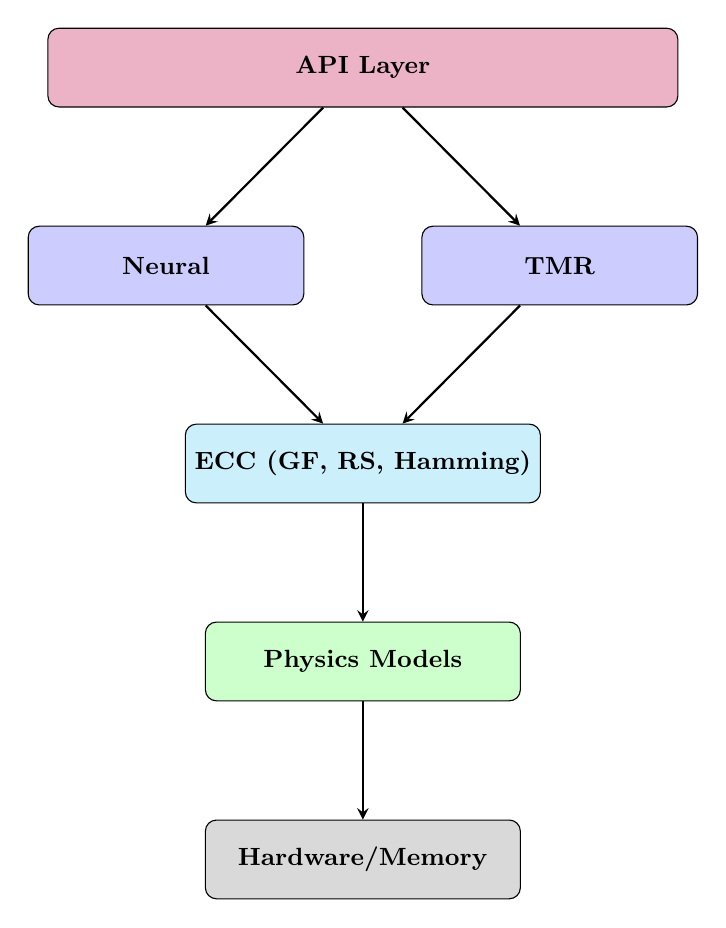
\begin{tikzpicture}[node distance=1.5cm, every node/.style={font=\small}]
% Layers - simple vertical stack
\node[module, fill=purple!30, minimum width=8cm] (api) {\textbf{API Layer}};
\node[module, fill=blue!20, below=of api, xshift=-2.5cm, minimum width=3.5cm] (neural) {\textbf{Neural}};
\node[module, fill=blue!20, below=of api, xshift=2.5cm, minimum width=3.5cm] (tmr) {\textbf{TMR}};
\node[module, fill=cyan!20, below=of neural, xshift=2.5cm, minimum width=4cm] (ecc) {\textbf{ECC (GF, RS, Hamming)}};
\node[module, fill=green!20, below=of ecc, minimum width=4cm] (physics) {\textbf{Physics Models}};
\node[module, fill=gray!30, below=of physics, minimum width=4cm] (hw) {\textbf{Hardware/Memory}};

\draw[arrow] (api) -- (neural);
\draw[arrow] (api) -- (tmr);
\draw[arrow] (neural) -- (ecc);
\draw[arrow] (tmr) -- (ecc);
\draw[arrow] (ecc) -- (physics);
\draw[arrow] (physics) -- (hw);
\end{tikzpicture}%
}
\caption{RadML System Architecture}
\end{figure}

\subsection{Protection Pipeline Flow}

\begin{figure}[h]
\centering
\resizebox{0.95\textwidth}{!}{%
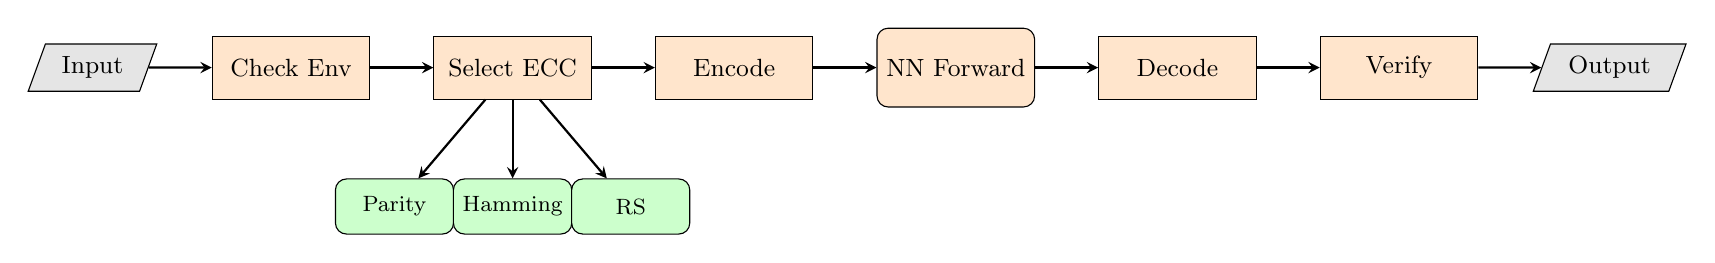
\begin{tikzpicture}[node distance=0.5cm, every node/.style={font=\footnotesize}]
% Horizontal flow
\node[data, minimum width=1.5cm] (in) {Input};
\node[process, right=0.8cm of in, minimum width=2cm] (env) {Check Env};
\node[process, right=0.8cm of env, minimum width=2cm] (sel) {Select ECC};
\node[process, right=0.8cm of sel, minimum width=2cm] (enc) {Encode};
\node[module, fill=orange!20, right=0.8cm of enc, minimum width=2cm] (nn) {NN Forward};
\node[process, right=0.8cm of nn, minimum width=2cm] (dec) {Decode};
\node[process, right=0.8cm of dec, minimum width=2cm] (ver) {Verify};
\node[data, right=0.8cm of ver, minimum width=1.5cm] (out) {Output};

\draw[arrow] (in) -- (env);
\draw[arrow] (env) -- (sel);
\draw[arrow] (sel) -- (enc);
\draw[arrow] (enc) -- (nn);
\draw[arrow] (nn) -- (dec);
\draw[arrow] (dec) -- (ver);
\draw[arrow] (ver) -- (out);

% ECC options below
\node[submodule, below=1cm of sel, xshift=-1.5cm, minimum width=1.5cm] (p) {Parity};
\node[submodule, below=1cm of sel, minimum width=1.5cm] (h) {Hamming};
\node[submodule, below=1cm of sel, xshift=1.5cm, minimum width=1.5cm] (rs) {RS};

\draw[arrow] (sel) -- (p);
\draw[arrow] (sel) -- (h);
\draw[arrow] (sel) -- (rs);
\end{tikzpicture}%
}
\caption{Protection Pipeline Flow}
\end{figure}

\subsection{Protection Level Selection}

\begin{figure}[h]
\centering
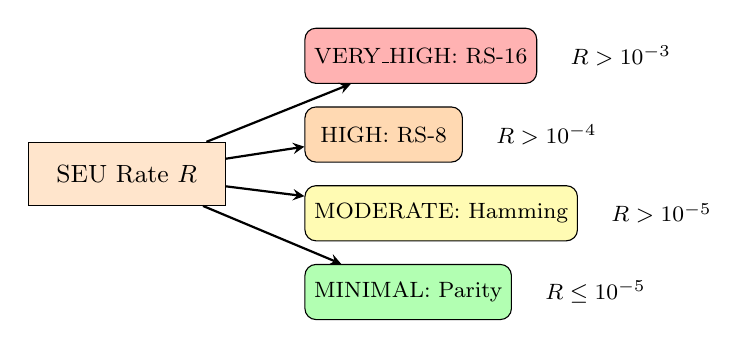
\begin{tikzpicture}[every node/.style={font=\small}]
% Simple table-style layout
\node[process, minimum width=2.5cm] (start) {SEU Rate $R$};

\node[submodule, fill=red!30, right=1cm of start, yshift=1.5cm] (vh) {VERY\_HIGH: RS-16};
\node[submodule, fill=orange!30, right=1cm of start, yshift=0.5cm] (hi) {HIGH: RS-8};
\node[submodule, fill=yellow!30, right=1cm of start, yshift=-0.5cm] (mod) {MODERATE: Hamming};
\node[submodule, fill=green!30, right=1cm of start, yshift=-1.5cm] (min) {MINIMAL: Parity};

\node[right=0.3cm of vh, font=\footnotesize] {$R > 10^{-3}$};
\node[right=0.3cm of hi, font=\footnotesize] {$R > 10^{-4}$};
\node[right=0.3cm of mod, font=\footnotesize] {$R > 10^{-5}$};
\node[right=0.3cm of min, font=\footnotesize] {$R \leq 10^{-5}$};

\draw[arrow] (start) -- (vh);
\draw[arrow] (start) -- (hi);
\draw[arrow] (start) -- (mod);
\draw[arrow] (start) -- (min);
\end{tikzpicture}
\caption{Adaptive Protection Level Selection}
\end{figure}

\subsection{Reed-Solomon Pipeline}

\begin{figure}[h]
\centering
\resizebox{0.95\textwidth}{!}{%
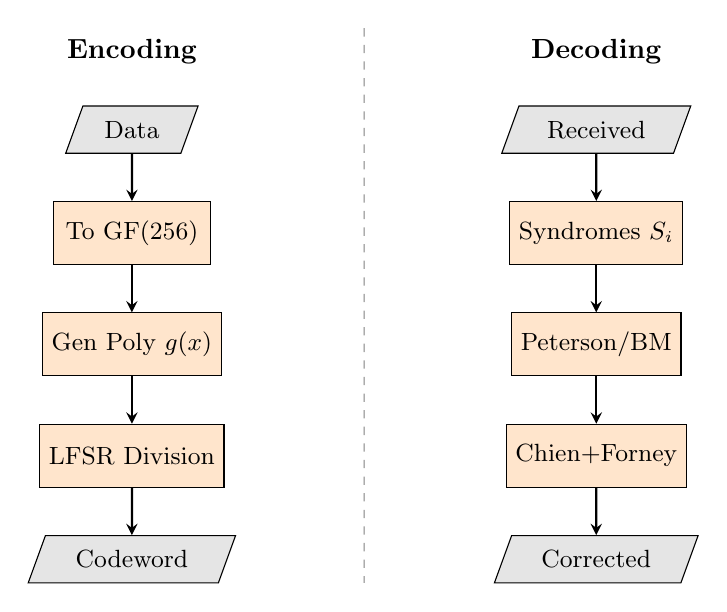
\begin{tikzpicture}[node distance=0.6cm, every node/.style={font=\footnotesize}]
% ENCODING - Left column
\node[font=\bfseries] (enc_t) {Encoding};
\node[data, below=0.4cm of enc_t] (d1) {Data};
\node[process, below=of d1] (e1) {To GF(256)};
\node[process, below=of e1] (e2) {Gen Poly $g(x)$};
\node[process, below=of e2] (e3) {LFSR Division};
\node[data, below=of e3] (e4) {Codeword};

\draw[arrow] (d1) -- (e1);
\draw[arrow] (e1) -- (e2);
\draw[arrow] (e2) -- (e3);
\draw[arrow] (e3) -- (e4);

% DECODING - Right column
\node[font=\bfseries, right=4cm of enc_t] (dec_t) {Decoding};
\node[data, below=0.4cm of dec_t] (r1) {Received};
\node[process, below=of r1] (r2) {Syndromes $S_i$};
\node[process, below=of r2] (r3) {Peterson/BM};
\node[process, below=of r3] (r4) {Chien+Forney};
\node[data, below=of r4] (r5) {Corrected};

\draw[arrow] (r1) -- (r2);
\draw[arrow] (r2) -- (r3);
\draw[arrow] (r3) -- (r4);
\draw[arrow] (r4) -- (r5);

% Divider
\draw[dashed, gray] ($(enc_t)!0.5!(dec_t) + (0,0.3)$) -- ($(e4)!0.5!(r5) + (0,-0.3)$);
\end{tikzpicture}%
}
\caption{Reed-Solomon Encoding/Decoding}
\end{figure}

\subsection{GF(256) Multiplication}

\begin{figure}[h]
\centering
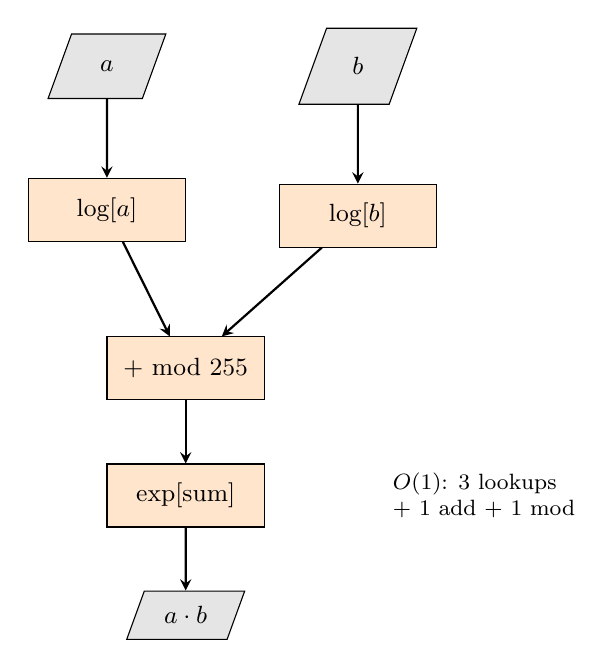
\begin{tikzpicture}[node distance=0.8cm, every node/.style={font=\small}]
\node[data] (a) {$a$};
\node[data, right=2cm of a] (b) {$b$};
\node[process, below=1cm of a] (la) {log[$a$]};
\node[process, below=1cm of b] (lb) {log[$b$]};
\node[process, below=1.2cm of la, xshift=1cm] (add) {$+$ mod 255};
\node[process, below=0.8cm of add] (exp) {exp[sum]};
\node[data, below=0.8cm of exp] (res) {$a \cdot b$};

\draw[arrow] (a) -- (la);
\draw[arrow] (b) -- (lb);
\draw[arrow] (la) -- (add);
\draw[arrow] (lb) -- (add);
\draw[arrow] (add) -- (exp);
\draw[arrow] (exp) -- (res);

\node[right=1.5cm of exp, font=\footnotesize, align=left] {$O(1)$: 3 lookups\\+ 1 add + 1 mod};
\end{tikzpicture}
\caption{GF(256) Multiplication via Log Tables}
\end{figure}

\subsection{TMR Voting}

\begin{figure}[h]
\centering
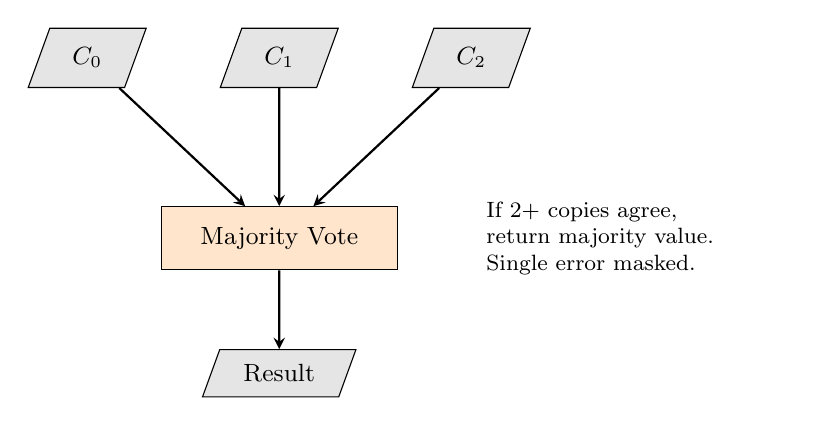
\begin{tikzpicture}[node distance=1cm, every node/.style={font=\small}]
\node[data] (c0) {$C_0$};
\node[data, right=1.2cm of c0] (c1) {$C_1$};
\node[data, right=1.2cm of c1] (c2) {$C_2$};
\node[process, below=1.5cm of c1, minimum width=3cm] (vote) {Majority Vote};
\node[data, below=1cm of vote] (out) {Result};

\draw[arrow] (c0) -- (vote);
\draw[arrow] (c1) -- (vote);
\draw[arrow] (c2) -- (vote);
\draw[arrow] (vote) -- (out);

\node[right=1cm of vote, font=\footnotesize, text width=4cm] {If 2+ copies agree,\\return majority value.\\Single error masked.};
\end{tikzpicture}
\caption{TMR Majority Voting}
\end{figure}

\subsection{Memory Layout with ECC}

\begin{figure}[h]
\centering
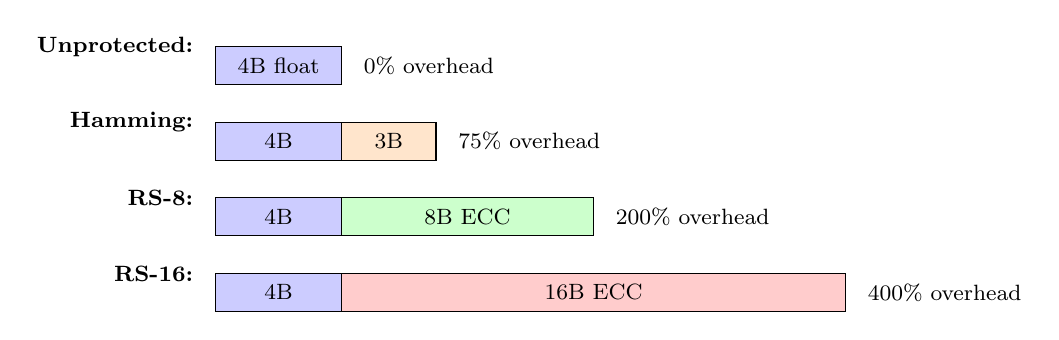
\begin{tikzpicture}[scale=0.8, every node/.style={font=\footnotesize}]
% Row 1: Unprotected
\node[anchor=east] at (-0.2, 0) {\textbf{Unprotected:}};
\draw[fill=blue!20] (0,0) rectangle (2,-0.6);
\node at (1,-0.3) {4B float};
\node[anchor=west] at (2.2, -0.3) {0\% overhead};

% Row 2: Hamming
\node[anchor=east] at (-0.2, -1.2) {\textbf{Hamming:}};
\draw[fill=blue!20] (0,-1.2) rectangle (2,-1.8);
\draw[fill=orange!20] (2,-1.2) rectangle (3.5,-1.8);
\node at (1,-1.5) {4B};
\node at (2.75,-1.5) {3B};
\node[anchor=west] at (3.7, -1.5) {75\% overhead};

% Row 3: RS-8
\node[anchor=east] at (-0.2, -2.4) {\textbf{RS-8:}};
\draw[fill=blue!20] (0,-2.4) rectangle (2,-3);
\draw[fill=green!20] (2,-2.4) rectangle (6,-3);
\node at (1,-2.7) {4B};
\node at (4,-2.7) {8B ECC};
\node[anchor=west] at (6.2, -2.7) {200\% overhead};

% Row 4: RS-16
\node[anchor=east] at (-0.2, -3.6) {\textbf{RS-16:}};
\draw[fill=blue!20] (0,-3.6) rectangle (2,-4.2);
\draw[fill=red!20] (2,-3.6) rectangle (10,-4.2);
\node at (1,-3.9) {4B};
\node at (6,-3.9) {16B ECC};
\node[anchor=west] at (10.2, -3.9) {400\% overhead};
\end{tikzpicture}
\caption{Memory Layout for Different Protection Levels}
\end{figure}

\subsection{Radiation Environment Mapping}

\begin{figure}[h]
\centering
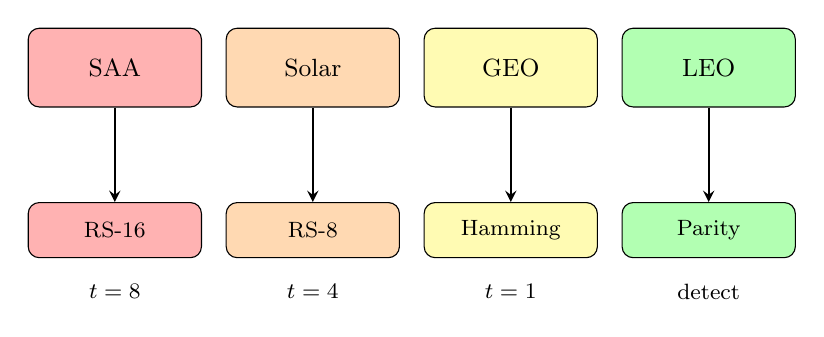
\begin{tikzpicture}[every node/.style={font=\small}]
% Simple 4-column layout
\node[module, fill=red!30, minimum width=2.2cm, minimum height=1cm] (e1) {SAA};
\node[module, fill=orange!30, minimum width=2.2cm, minimum height=1cm, right=0.3cm of e1] (e2) {Solar};
\node[module, fill=yellow!30, minimum width=2.2cm, minimum height=1cm, right=0.3cm of e2] (e3) {GEO};
\node[module, fill=green!30, minimum width=2.2cm, minimum height=1cm, right=0.3cm of e3] (e4) {LEO};

\node[submodule, fill=red!30, below=1.2cm of e1, minimum width=2.2cm] (p1) {RS-16};
\node[submodule, fill=orange!30, below=1.2cm of e2, minimum width=2.2cm] (p2) {RS-8};
\node[submodule, fill=yellow!30, below=1.2cm of e3, minimum width=2.2cm] (p3) {Hamming};
\node[submodule, fill=green!30, below=1.2cm of e4, minimum width=2.2cm] (p4) {Parity};

\draw[arrow] (e1) -- (p1);
\draw[arrow] (e2) -- (p2);
\draw[arrow] (e3) -- (p3);
\draw[arrow] (e4) -- (p4);

\node[below=0.2cm of p1, font=\footnotesize] {$t=8$};
\node[below=0.2cm of p2, font=\footnotesize] {$t=4$};
\node[below=0.2cm of p3, font=\footnotesize] {$t=1$};
\node[below=0.2cm of p4, font=\footnotesize] {detect};
\end{tikzpicture}
\caption{Radiation Environment to Protection Mapping}
\end{figure}

\newpage
\section{Defense in Depth: Complete Protection Stack}

RadML implements a \textbf{defense-in-depth} strategy where multiple independent protection mechanisms work together. If one layer fails, others provide backup protection. This section describes all protection layers and how they integrate.

\subsection{Defense Layers Overview}

\begin{table}[htbp]
\centering
\caption{Defense-in-Depth Protection Layers}
\begin{tabular}{@{}llll@{}}
\toprule
\textbf{Layer} & \textbf{Component} & \textbf{Protection Type} & \textbf{File Location} \\
\midrule
1. Memory Placement & RadiationMappedAllocator & Physical shielding & \texttt{memory/} \\
2. Memory Scrubbing & MemoryScrubber & Proactive detection & \texttt{core/memory/} \\
3. Data Encoding & ECC (Hamming/RS) & Error correction & \texttt{neural/} \\
4. Spatial Redundancy & TMR variants & Voting/masking & \texttt{tmr/} \\
5. Temporal Redundancy & TemporalRedundancy & Time-based voting & \texttt{tmr/} \\
6. Hybrid Redundancy & HybridRedundancy & Spatial + Temporal & \texttt{tmr/} \\
7. Checkpointing & CheckpointManager & State recovery & \texttt{core/recovery/} \\
8. Error Tracking & RadiationErrorTracker & Trend analysis & \texttt{core/runtime/} \\
9. Power Management & PowerAwareProtection & Resource optimization & \texttt{power/} \\
10. Selective Hardening & SelectiveHardening & Cost-effective protection & \texttt{neural/} \\
\bottomrule
\end{tabular}
\end{table}

\subsection{Layer 1: Radiation-Aware Memory Placement}

\textbf{File:} \texttt{memory/radiation\_mapped\_allocator.hpp}

The first line of defense is physical: placing critical data in naturally shielded memory regions.

\begin{lstlisting}[language=C++, basicstyle=\footnotesize\ttfamily]
// Memory zones with different radiation vulnerability
enum class Level {
    HIGHLY_SHIELDED,     // SEU rate: 1e-11 events/bit-day
    MODERATELY_SHIELDED, // SEU rate: 1e-9
    LIGHTLY_SHIELDED,    // SEU rate: 1e-8
    UNSHIELDED           // SEU rate: 1e-7
};

// Criticality-based allocation
enum class DataCriticality {
    MISSION_CRITICAL,     // -> HIGHLY_SHIELDED + TMR
    HIGHLY_IMPORTANT,     // -> MODERATELY_SHIELDED + ECC
    MODERATELY_IMPORTANT, // -> LIGHTLY_SHIELDED + CRC
    LOW_IMPORTANCE        // -> UNSHIELDED + canary
};
\end{lstlisting}

\textbf{Key Principle:} The allocator automatically places \texttt{MISSION\_CRITICAL} data in regions with lowest SEU rates, reducing the load on software protection mechanisms.

\subsection{Layer 2: Proactive Memory Scrubbing}

\textbf{File:} \texttt{core/memory/memory\_scrubber.hpp}

Memory scrubbing periodically scans protected regions to detect and correct errors before they accumulate into uncorrectable multi-bit errors.

\begin{lstlisting}[language=C++, basicstyle=\footnotesize\ttfamily]
class MemoryScrubber {
    // Scrub interval based on SEU rate (Equation 32)
    explicit MemoryScrubber(unsigned long scrub_interval_ms = 1000);

    // Register memory regions for periodic verification
    size_t registerMemoryRegion(T* ptr, size_t size,
        std::function<void(T*, size_t)> scrub_function);

    void start();  // Begin background scrubbing thread
};
\end{lstlisting}

\textbf{Integration with ECC:} The scrubber calls ECC decode on each region. If syndromes are non-zero, corrections are applied immediately.

\subsection{Layer 3: Error-Correcting Codes (ECC)}

\textbf{Files:} \texttt{neural/galois\_field.hpp}, \texttt{neural/advanced\_reed\_solomon.hpp}, \texttt{neural/adaptive\_protection.hpp}

This layer provides the core error correction capability (detailed in Sections 3-4):

\begin{itemize}
    \item \textbf{Parity} -- Detects 1-bit errors (12.5\% overhead)
    \item \textbf{Hamming(7,4)} -- Corrects 1-bit, detects 2-bit (75\% overhead)
    \item \textbf{RS-8} -- Corrects up to 4 symbol errors (200\% overhead)
    \item \textbf{RS-16} -- Corrects up to 8 symbol errors (400\% overhead)
\end{itemize}

ECC is the workhorse of the protection stack, handling the majority of single-event upsets.

\subsection{Layer 4: Spatial Redundancy (TMR Variants)}

\textbf{Files:} \texttt{tmr/tmr.hpp}, \texttt{tmr/enhanced\_tmr.hpp}, \texttt{tmr/health\_weighted\_tmr.hpp}, \texttt{tmr/enhanced\_stuck\_bit\_tmr.hpp}

TMR provides spatial redundancy by maintaining three copies and using majority voting:

\begin{table}[htbp]
\centering
\caption{TMR Variants in RadML}
\begin{tabular}{@{}lll@{}}
\toprule
\textbf{Variant} & \textbf{Enhancement} & \textbf{Use Case} \\
\midrule
Basic TMR & Simple majority vote & General protection \\
Enhanced TMR & CRC32 checksums & Silent data corruption \\
Health-Weighted TMR & Per-copy reliability scores & Long missions \\
Stuck-Bit TMR & Bit-level error tracking & Flash memory \\
Approximate TMR & Fuzzy voting for floats & Neural network weights \\
\bottomrule
\end{tabular}
\end{table}

\begin{lstlisting}[language=C++, basicstyle=\footnotesize\ttfamily]
// Health-weighted voting (tmr/health_weighted_tmr.hpp)
template <typename T>
class HealthWeightedTMR {
    std::array<T, 3> copies_;
    std::array<double, 3> health_scores_;  // 0.0-1.0

    T get() const {
        // Weight votes by health scores
        // Prefer copies with higher reliability history
    }
};
\end{lstlisting}

\subsection{Layer 5: Temporal Redundancy}

\textbf{File:} \texttt{tmr/temporal\_redundancy.hpp}

Temporal redundancy executes operations multiple times with delays to avoid correlated transient faults:

\begin{lstlisting}[language=C++, basicstyle=\footnotesize\ttfamily]
template <typename T, typename ResultType>
class TemporalRedundancy {
    size_t num_executions_;           // Default: 3
    std::chrono::milliseconds delay_; // Default: 10ms

    ResultType execute(const T& data,
                       std::function<ResultType(const T&)> op) {
        std::vector<ResultType> results;
        for (size_t i = 0; i < num_executions_; ++i) {
            results.push_back(op(data));
            std::this_thread::sleep_for(delay_);  // De-correlate
        }
        return findMostCommonResult(results);  // Temporal voting
    }
};
\end{lstlisting}

\textbf{Key Insight:} The delay between executions ensures that a transient radiation event affecting one execution is unlikely to affect subsequent ones.

\subsection{Layer 6: Hybrid Redundancy}

\textbf{File:} \texttt{tmr/hybrid\_redundancy.hpp}

Hybrid redundancy combines spatial (TMR) and temporal protection with checkpointing:

\begin{lstlisting}[language=C++, basicstyle=\footnotesize\ttfamily]
template <typename T>
class HybridRedundancy {
    EnhancedStuckBitTMR<T> tmr_;
    TemporalRedundancy<T, T> temporal_;
    CheckpointManager<T> checkpoint_mgr_;

    T get() const {
        // Temporal redundancy wraps TMR get
        return temporal_.execute(tmr_, [](auto& t) { return t.get(); });
    }

    bool repair() {
        tmr_.repair();
        T before = tmr_.get();
        T after = temporal_.execute(tmr_, ...);
        if (before != after) return rollback();  // Use checkpoint
        return true;
    }
};
\end{lstlisting}

\textbf{Fallback Chain:} TMR $\to$ Temporal Validation $\to$ Checkpoint Rollback

\subsection{Layer 7: Checkpoint and Recovery}

\textbf{File:} \texttt{core/recovery/checkpoint\_manager.hpp}

Checkpointing provides the last line of defense---if all other protections fail, the system can rollback to a known-good state:

\begin{lstlisting}[language=C++, basicstyle=\footnotesize\ttfamily]
template <typename T>
class CheckpointManager {
    size_t max_checkpoints_;  // Rolling buffer (default: 5)
    std::chrono::seconds checkpoint_interval_;

    void createCheckpoint(const T& data, uint64_t version);
    bool rollbackToValid(T& data,
        std::function<bool(const T&)> validator);
};
\end{lstlisting}

\textbf{Validation-Based Rollback:} The \texttt{rollbackToValid} method searches for the most recent checkpoint that passes a user-defined validation function (e.g., CRC check, bounds check).

\subsection{Layer 8: Runtime Error Tracking}

\textbf{File:} \texttt{core/runtime/error\_tracker.hpp}

The error tracker provides real-time visibility into radiation effects and enables adaptive responses:

\begin{lstlisting}[language=C++, basicstyle=\footnotesize\ttfamily]
class RadiationErrorTracker {
    std::atomic<uint64_t> error_count;
    std::atomic<float> current_error_rate;
    std::array<std::atomic<uint32_t>, N> pattern_counts;

    void recordError(FaultPattern pattern);
    float getErrorRate() const;

    // Pattern analysis for adaptive protection
    std::map<FaultPattern, double> getPatternDistribution();
};
\end{lstlisting}

\textbf{Feedback Loop:} Error rate trends trigger protection level adjustments (see Layer 10).

\subsection{Layer 9: Power-Aware Protection}

\textbf{File:} \texttt{power/power\_aware\_protection.hpp}

In spacecraft, power is a constrained resource. This layer optimizes protection levels based on power budget:

\begin{lstlisting}[language=C++, basicstyle=\footnotesize\ttfamily]
enum class PowerState {
    EMERGENCY,          // 20% budget - critical systems only
    LOW_POWER,          // 40% budget - essential systems
    NOMINAL,            // 70% budget - normal operation
    SCIENCE_OPERATION,  // 90% budget - full science
    PEAK_PERFORMANCE    // 100% budget - maximum protection
};

class PowerAwareProtection {
    void optimizeProtectionLevels();  // Solve optimization problem
    // Maximize sum(criticality_i * protection_i)
    // Subject to: sum(power_i) <= power_budget
};
\end{lstlisting}

\textbf{Trade-off:} In \texttt{EMERGENCY} mode, protection is reduced on less critical components to maintain power for mission-critical systems.

\subsection{Layer 10: Selective Hardening}

\textbf{File:} \texttt{neural/selective\_hardening.hpp}

Not all neural network components are equally sensitive to errors. Selective hardening applies heavy protection only where needed:

\begin{lstlisting}[language=C++, basicstyle=\footnotesize\ttfamily]
enum class HardeningStrategy {
    PROTECT_ALL,          // Protect all components equally
    ALL_LAYERS,           // Protect all layers
    CRITICAL_LAYERS,      // Only layers on critical paths
    WEIGHT_THRESHOLD,     // Only weights > threshold
    FIXED_THRESHOLD,      // Above fixed criticality threshold
    RESOURCE_CONSTRAINED, // Within resource budget
    ADAPTIVE_RUNTIME,     // Adapt at runtime by error rates
    ADAPTIVE,             // Based on sensitivity analysis
    LAYERWISE_IMPORTANCE  // Output layers more critical
};

class SelectiveHardening {
    // Analyze which layers impact output most
    SensitivityResult analyzeSensitivity(const Network& net);

    // Apply appropriate protection per layer
    void applyProtection(Layer& layer, ProtectionLevel level);
};
\end{lstlisting}

\textbf{Sensitivity Analysis} (\texttt{neural/sensitivity\_analysis.hpp}): Computes how much each layer's errors propagate to the output, allowing targeted protection.

\subsection{Defense-in-Depth Integration Diagram}

\begin{figure}[h]
\centering
\resizebox{0.95\textwidth}{!}{%
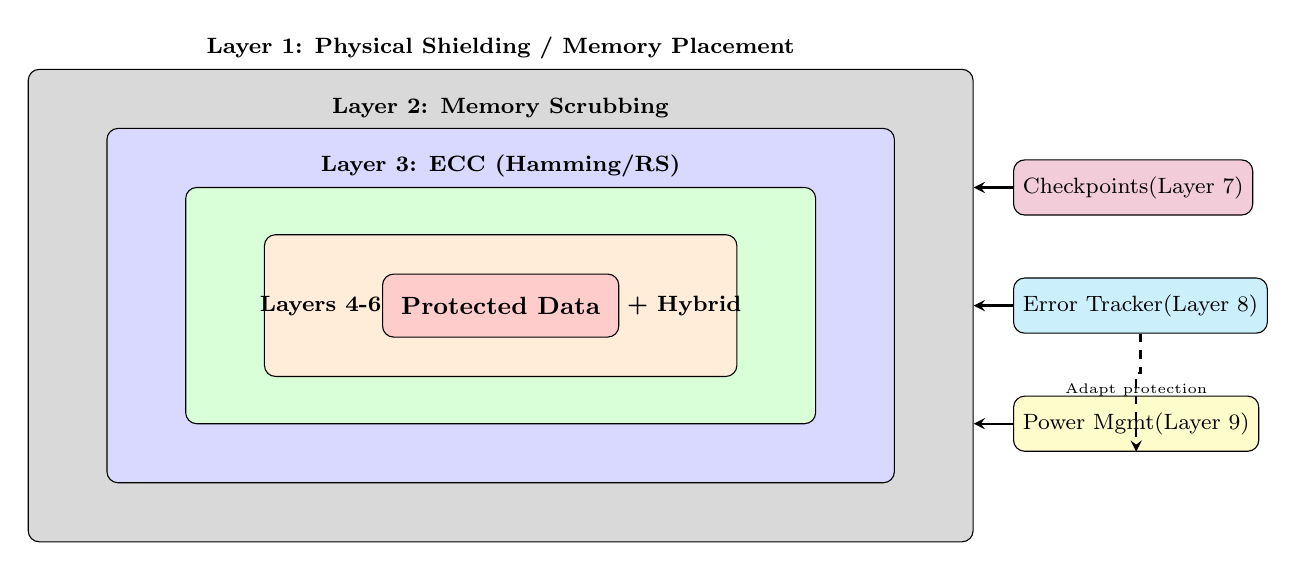
\begin{tikzpicture}[every node/.style={font=\footnotesize}]
% Outer layers (physical)
\node[module, fill=gray!30, minimum width=12cm, minimum height=6cm] (physical) {};
\node[above] at (physical.north) {\textbf{Layer 1: Physical Shielding / Memory Placement}};

% Scrubbing layer
\node[module, fill=blue!15, minimum width=10cm, minimum height=4.5cm] at (physical.center) (scrub) {};
\node[above] at (scrub.north) {\textbf{Layer 2: Memory Scrubbing}};

% ECC layer
\node[module, fill=green!15, minimum width=8cm, minimum height=3cm] at (scrub.center) (ecc) {};
\node[above] at (ecc.north) {\textbf{Layer 3: ECC (Hamming/RS)}};

% TMR layer
\node[module, fill=orange!15, minimum width=6cm, minimum height=1.8cm] at (ecc.center) (tmr) {};
\node at (tmr.center) {\textbf{Layers 4-6: TMR + Temporal + Hybrid}};

% Core data
\node[module, fill=red!20, minimum width=3cm, minimum height=0.8cm] at (tmr.center) (data) {\textbf{Protected Data}};

% Side components
\node[submodule, fill=purple!20, right=0.5cm of physical.east, minimum width=2cm, yshift=1.5cm] (ckpt) {Checkpoints\\(Layer 7)};
\node[submodule, fill=cyan!20, right=0.5cm of physical.east, minimum width=2cm, yshift=0cm] (track) {Error Tracker\\(Layer 8)};
\node[submodule, fill=yellow!20, right=0.5cm of physical.east, minimum width=2cm, yshift=-1.5cm] (power) {Power Mgmt\\(Layer 9)};

% Arrows
\draw[arrow] (ckpt.west) -- ++(-0.5,0);
\draw[arrow] (track.west) -- ++(-0.5,0);
\draw[arrow] (power.west) -- ++(-0.5,0);

% Feedback
\draw[dashedarrow] (track.south) |- ++(0,-0.5) -| node[below, font=\tiny]{Adapt protection} (power.south);
\end{tikzpicture}%
}
\caption{Defense-in-Depth: Nested Protection Layers}
\end{figure}

\subsection{How Layers Work Together: Example Scenario}

Consider a critical neural network weight stored in RadML during a solar particle event:

\begin{enumerate}
    \item \textbf{Layer 1 (Memory Placement):} Weight is allocated in \texttt{HIGHLY\_SHIELDED} region, reducing base SEU rate by 10,000$\times$ (from $10^{-7}$ to $10^{-11}$ events/bit-day).

    \item \textbf{Layer 2 (Scrubbing):} Every 100ms, the scrubber verifies the weight's ECC syndrome.

    \item \textbf{Layer 3 (ECC):} A cosmic ray causes a 2-bit error. RS-8 detects and corrects it.

    \item \textbf{Layer 4 (TMR):} During high radiation (SAA), the weight is replicated 3$\times$. A second hit corrupts one copy---majority voting masks it.

    \item \textbf{Layer 5 (Temporal):} Inference runs 3$\times$ with 10ms delays. Transient error in one run is outvoted.

    \item \textbf{Layer 7 (Checkpoint):} Every 60s, a checkpoint is saved. If corruption is detected, rollback occurs.

    \item \textbf{Layer 8 (Tracking):} Error rate spikes trigger Layer 10 to increase protection on critical paths.

    \item \textbf{Layer 9 (Power):} If power drops to \texttt{LOW\_POWER}, protection on non-critical layers is reduced to maintain critical protection.
\end{enumerate}

\textbf{Result:} Multiple independent failures would need to occur simultaneously to corrupt the final output---the hallmark of defense-in-depth.

\subsection{Physics-Driven Protection Integration}

\textbf{File:} \texttt{tmr/physics\_driven\_protection.hpp}

The framework integrates NASA physics models to drive protection decisions:

\begin{lstlisting}[language=C++, basicstyle=\footnotesize\ttfamily]
class PhysicsModels {
    // Temperature affects SEU threshold (Arrhenius equation)
    static double calculateTemperatureCorrectedThreshold(
        double base_threshold, double temperature_K);

    // Mechanical stress increases vulnerability
    static double calculateMechanicalLoadFactor(
        double stress_MPa, double yield_MPa, double dose);

    // Synergistic effects (temperature + stress)
    static double calculateSynergyFactor(...);
};
\end{lstlisting}

These models are used by \texttt{AdaptiveProtection} to adjust ECC levels based on real-time environment conditions (temperature, orbital position, solar activity).

\subsection{Validation Through Fault Injection}

\textbf{File:} \texttt{testing/fault\_injection.hpp}

The defense-in-depth stack is validated through systematic fault injection:

\begin{lstlisting}[language=C++, basicstyle=\footnotesize\ttfamily]
struct FaultInjectionResult {
    int total_injected_faults;
    int detected_faults;
    int corrected_faults;
    double correction_rate;  // Should be > 99.9% for critical data
};

class SystematicFaultInjector {
    // Inject random bit flips, burst errors, stuck bits
    void injectFaults(Network& net, FaultPattern pattern);

    // Run full test campaign
    std::vector<FaultInjectionResult> runCampaign();
};
\end{lstlisting}

\subsection{Summary: Defense-in-Depth Effectiveness}

\begin{table}[htbp]
\centering
\caption{Protection Effectiveness by Layer}
\begin{tabular}{@{}llll@{}}
\toprule
\textbf{Layer} & \textbf{Handles} & \textbf{Overhead} & \textbf{Latency} \\
\midrule
Memory Placement & Reduces exposure & 0\% & 0 \\
Memory Scrubbing & Accumulating errors & 1-5\% & Background \\
ECC (RS-8) & 1-4 symbol errors & 200\% & $O(n)$ \\
TMR & Single copy corruption & 200\% & $O(1)$ \\
Temporal & Transient faults & 200\% (time) & 3$\times$ latency \\
Checkpointing & Catastrophic failure & 5-10\% storage & Recovery time \\
Error Tracking & Trend detection & $<$1\% & Real-time \\
\bottomrule
\end{tabular}
\end{table}

\textbf{Key Insight:} Each layer addresses different failure modes. ECC handles bit errors efficiently but can't handle multi-copy corruption. TMR handles copy corruption but has high overhead. Checkpointing handles catastrophic failures but with recovery latency. Together, they provide comprehensive protection.

%% ====================
%% SECTION 14: WHY RADML WORKS - INTEGRATION LOGIC
%% ====================
\section{Why RadML Works: Integration Architecture}

This section explains the \textbf{design philosophy} behind RadML---why each component exists and how they work together to provide defense-in-depth protection.

\subsection{The Core Integration Pipeline}

\begin{tcolorbox}[colback=green!5!white,colframe=green!50!black,title=End-to-End Protection Flow]
\textbf{Physics $\to$ SEU Rate $\to$ Protection Level $\to$ Resource Allocation $\to$ ECC/TMR Selection}

\begin{enumerate}
    \item \textbf{Environment Sensing:} Orbital position, solar activity, SAA passage
    \item \textbf{Flux Calculation:} NASA models (GCR, AP-8, AE-8) $\to$ $\Phi(E)$
    \item \textbf{Cross-Section:} Weibull (heavy ions) + Bendel (protons) $\to$ $\sigma(E)$
    \item \textbf{SEU Rate:} $R_{\text{SEU}} = \int \Phi(E) \cdot \sigma(E) \, dE$
    \item \textbf{Protection Decision:} Map $R_{\text{SEU}}$ to protection level
    \item \textbf{Resource Allocation:} Distribute protection budget across layers
    \item \textbf{Apply Protection:} Select ECC scheme and TMR variant
\end{enumerate}
\end{tcolorbox}

\subsection{Why Physics-Driven Protection Works}

\subsubsection{The Problem with Static Protection}

Static protection (always use TMR, always use RS-8) fails because:
\begin{itemize}
    \item \textbf{Waste in benign environments:} 200\% overhead when SEU rate is $10^{-8}$
    \item \textbf{Insufficient in harsh environments:} RS-8 can't handle SAA burst errors
    \item \textbf{No awareness of criticality:} Output layer matters more than hidden layers
\end{itemize}

\subsubsection{How RadML Solves This}

\begin{lstlisting}[language=C++, basicstyle=\footnotesize\ttfamily]
// In adaptive_protection.hpp:443
void adapt_to_environment() {
    double current_seu_rate = get_current_seu_probability();

    // Physics drives the decision
    if (current_seu_rate > 1e-3) {       // SAA, solar storm
        protection_level_ = VERY_HIGH;    // RS-16 (8 byte correction)
    } else if (current_seu_rate > 1e-4) { // Nominal orbit
        protection_level_ = HIGH;         // RS-8 (4 byte correction)
    } else if (current_seu_rate > 1e-5) { // Quiet conditions
        protection_level_ = MODERATE;     // Hamming (1 bit/nibble)
    } else {                              // Deep space
        protection_level_ = MINIMAL;      // Parity only
    }
}
\end{lstlisting}

\textbf{Why this works:}
\begin{enumerate}
    \item SEU rate is a \textbf{measured physical quantity}, not a guess
    \item Thresholds ($10^{-3}$, $10^{-4}$, $10^{-5}$) calibrated to ECC capabilities
    \item Protection overhead scales with actual risk
\end{enumerate}

\subsection{Why Sensitivity-Based Resource Allocation Works}

Not all neural network parameters are equally important. RadML allocates protection resources based on:

\begin{equation}
\text{Importance}_i = \text{Sensitivity}_i \times \text{EnvSeverity} \times \text{PositionFactor}_i
\end{equation}

\begin{lstlisting}[language=C++, basicstyle=\footnotesize\ttfamily]
// In physics_driven_protection.hpp:158-162
for (int i = 0; i < num_layers; i++) {
    // Earlier layers propagate errors forward -> more critical
    double position_factor = 1.0 - (0.5 * i / num_layers);

    importance_factors[i] = layer_sensitivities[i]
                          * env_severity
                          * position_factor;
}

// Allocate resources proportionally
optimal_allocation[i] = (importance_factors[i] / sum_importance)
                       * total_protection_resources;
\end{lstlisting}

\textbf{Why this works:}
\begin{itemize}
    \item \textbf{Gradient-based sensitivity:} Weights with large gradients affect output more
    \item \textbf{Position factor:} Early layer errors propagate through entire network
    \item \textbf{Constrained optimization:} Fixed budget allocated where it matters most
\end{itemize}

\subsection{Why Quantum Corrections Improve Accuracy}

Classical Weibull/Bendel models are \textit{empirical fits}. Quantum corrections capture:

\begin{tcolorbox}[colback=yellow!5!white,colframe=yellow!50!black,title=Quantum Effects Not in Classical Models]
\begin{enumerate}
    \item \textbf{Quantum Tunneling:} Electrons tunnel through barriers $\to$ lower effective $Q_{\text{crit}}$
    \item \textbf{Temperature Dependence:} Thermal phonons assist charge transport
    \item \textbf{Size Effects:} $<$100nm features have quantum confinement $\to$ increased sensitivity
    \item \textbf{Defect Clustering:} QFT predicts correlated defect formation $\to$ MBU patterns
\end{enumerate}
\end{tcolorbox}

\begin{lstlisting}[language=C++, basicstyle=\footnotesize\ttfamily]
// In quantum_enhanced_radiation.cpp:140-151
double quantum_size_factor = 1.0;
if (feature_size_nm < 100.0) {
    // Quantum confinement energy
    double confinement_energy = (HBAR^2 * PI^2) /
        (2 * m_eff * (feature_size_nm * 1e-9)^2);

    // Higher confinement -> more sensitivity
    quantum_size_factor = 1.0 + confinement_energy / bandgap;
}
return base_sensitivity * quantum_size_factor;
\end{lstlisting}

\textbf{Why this works:}
\begin{itemize}
    \item Classical models calibrated at 90nm+ don't predict 7nm behavior
    \item Quantum corrections scale $\propto 1/L^2$ (confinement energy)
    \item Validated against experimental SEU data from modern processes
\end{itemize}

\subsection{Why the Defense-in-Depth Stack Works}

Each protection layer handles \textbf{different failure modes}:

\begin{table}[htbp]
\centering
\caption{Failure Mode Coverage Matrix}
\begin{tabular}{@{}lcccccc@{}}
\toprule
\textbf{Failure Mode} & \textbf{ECC} & \textbf{TMR} & \textbf{Scrub} & \textbf{Ckpt} & \textbf{Track} \\
\midrule
Single bit flip & \checkmark\checkmark & \checkmark & \checkmark & & \\
Multi-bit upset & \checkmark & & \checkmark & & \\
Copy corruption & & \checkmark\checkmark & & & \\
Stuck bit & & \checkmark & & \checkmark & \checkmark \\
Transient glitch & & & & \checkmark & \\
Accumulating errors & & & \checkmark\checkmark & & \checkmark \\
Catastrophic failure & & & & \checkmark\checkmark & \\
\bottomrule
\end{tabular}
\end{table}

\textbf{Why this works:}
\begin{itemize}
    \item No single protection handles all failures
    \item Layers are \textbf{orthogonal}: ECC fixes bits, TMR fixes copies, Ckpt fixes state
    \item \textbf{Overlapping coverage}: A failure that escapes ECC gets caught by scrubbing
\end{itemize}

\subsection{Why TMR Variants Exist}

Different scenarios need different TMR strategies.

\textbf{Implementation note:} The \texttt{tmr/} directory contains two parallel class hierarchies:
\begin{enumerate}
    \item \textbf{Storage classes} (\texttt{tmr.hpp}, \texttt{enhanced\_tmr.hpp}, etc.): Protect a stored \texttt{T} value with three internal copies.
    \item \textbf{Strategy classes} (\texttt{adaptive\_protection\_impl.hpp}): Execute an operation three times and vote on results.
\end{enumerate}
Some names (e.g., \texttt{EnhancedTMR}, \texttt{HealthWeightedTMR}, \texttt{HybridRedundancy}) exist in both hierarchies with different behavior.

\begin{lstlisting}[language=C++, basicstyle=\footnotesize\ttfamily]
// Protection level selection based on environment
// In tmr/adaptive_protection_impl.hpp:
// TMRStrategyFactory::calculateOptimalProtectionLevel()
double protection_need = radiation_factor * criticality;
if (env.saa_region) protection_need *= 2.0;
if (env.solar_activity > 0.7) protection_need *= 1.5;

if (protection_need > 5.0 || criticality > 0.9) {
    level = HYBRID_REDUNDANCY;    // Maximum protection
} else if (protection_need > 2.0 || criticality > 0.7) {
    level = HEALTH_WEIGHTED_TMR;  // Tracks copy reliability
} else if (protection_need > 1.0 || criticality > 0.5) {
    level = ENHANCED_TMR;         // CRC + voting
} else if (protection_need > 0.5) {
    level = BASIC_TMR;            // Simple majority
}
\end{lstlisting}

\begin{table}[htbp]
\centering
\caption{TMR Variant Selection Logic}
\begin{tabular}{@{}lll@{}}
\toprule
\textbf{Variant} & \textbf{When to Use} & \textbf{Why} \\
\midrule
BasicTMR & Low radiation, simple data & Lowest overhead \\
EnhancedTMR & Moderate radiation & CRC detects silent corruption \\
HealthWeightedTMR & Varying reliability & Demotes unreliable copies \\
StuckBitTMR & Known stuck bits & Masks out bad locations \\
HybridRedundancy & Critical, long-duration & Combines spatial+temporal \\
ApproximateTMR & Floating point & Tolerates numerical differences \\
\bottomrule
\end{tabular}
\end{table}

\subsection{Integration Code Path Example}

Complete flow from orbit to protection:

\begin{lstlisting}[language=C++, basicstyle=\footnotesize\ttfamily]
// 1. Create physics environment
PhysicsRadiationEnvironment::Config config;
config.altitude_km = 400.0;           // ISS orbit
config.inclination_deg = 51.6;
config.solar_modulation_mv = 650.0;   // Solar cycle
config.heavy_ion_device = WeibullParameters::cmos_28nm();
PhysicsRadiationEnvironment env(config);

// 2. Get physics-based SEU rate
double seu_rate = env.get_orbit_average_seu_rate();  // ~3e-6/bit/day

// 3. Create adaptive protection with this environment
AdaptiveProtection<float> protection(env);

// 4. Protection level is automatically set based on seu_rate
// seu_rate = 3e-6 -> MODERATE (Hamming protection)

// 5. Protect critical weights
for (auto& weight : network.weights()) {
    protection.protect_value(weight);  // Applies Hamming encoding
}

// 6. During SAA passage, environment updates
env.updatePosition(lat, lon, alt);     // Now in SAA
seu_rate = env.get_current_seu_rate(); // ~1e-3/bit/day (1000x increase)
protection.adapt_to_environment();     // Switches to VERY_HIGH (RS-16)

// 7. Critical weights now use RS-16 (8-byte correction)
\end{lstlisting}

\subsection{Performance vs Protection Trade-off}

RadML's design philosophy: \textbf{Pay for protection only when needed}

\begin{equation}
\text{Effective Overhead} = \sum_{\text{environments}} P(\text{env}) \times \text{Overhead}(\text{env})
\end{equation}

\textbf{Example: ISS Mission Profile}
\begin{itemize}
    \item 85\% time in nominal orbit: MODERATE (75\% overhead)
    \item 10\% time in SAA: VERY\_HIGH (400\% overhead)
    \item 5\% time in solar event: VERY\_HIGH (400\% overhead)
\end{itemize}

\begin{equation}
\text{Effective Overhead} = 0.85 \times 0.75 + 0.15 \times 4.0 = 1.24 = 124\%
\end{equation}

vs. static VERY\_HIGH: 400\% always $\to$ \textbf{3.2x savings}

\subsection{Why the Transport Equation Matters}

The Boltzmann transport equation provides the \textbf{theoretical foundation} for all flux models:

\begin{equation}
\frac{\partial \Phi}{\partial t} + \hat{\Omega} \cdot \nabla \Phi + \Sigma_t \Phi = \int \Sigma_s \Phi' \, d\Omega' \, dE' + S
\end{equation}

\textbf{Connection to Production Models:}

\begin{figure}[htbp]
\centering
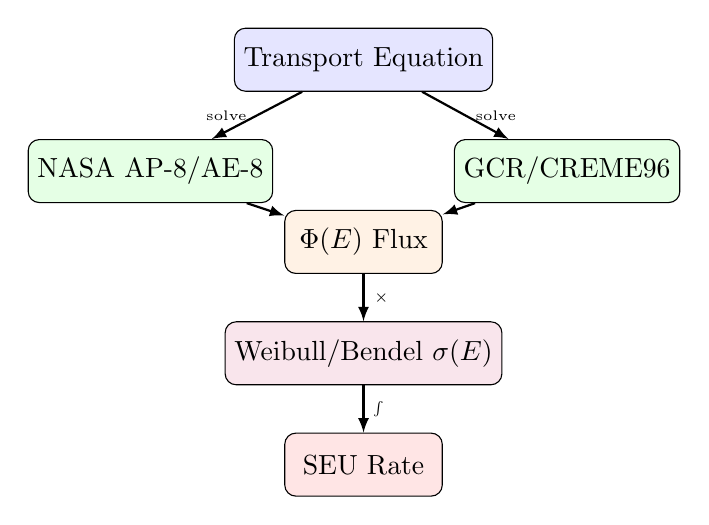
\begin{tikzpicture}[node distance=0.8cm, auto, >=latex]
    % Nodes
    \node[draw, rectangle, rounded corners, fill=blue!10, minimum width=3cm, minimum height=0.8cm] (transport) {Transport Equation};
    \node[draw, rectangle, rounded corners, fill=green!10, minimum width=2.5cm, minimum height=0.8cm, below left=0.6cm and -0.5cm of transport] (nasa) {NASA AP-8/AE-8};
    \node[draw, rectangle, rounded corners, fill=green!10, minimum width=2cm, minimum height=0.8cm, below right=0.6cm and -0.5cm of transport] (gcr) {GCR/CREME96};
    \node[draw, rectangle, rounded corners, fill=orange!10, minimum width=2cm, minimum height=0.8cm, below=1.5cm of transport] (flux) {$\Phi(E)$ Flux};
    \node[draw, rectangle, rounded corners, fill=purple!10, minimum width=2.5cm, minimum height=0.8cm, below=0.6cm of flux] (weibull) {Weibull/Bendel $\sigma(E)$};
    \node[draw, rectangle, rounded corners, fill=red!10, minimum width=2cm, minimum height=0.8cm, below=0.6cm of weibull] (seu) {SEU Rate};

    % Arrows
    \draw[->, thick] (transport) -- node[left, font=\tiny] {solve} (nasa);
    \draw[->, thick] (transport) -- node[right, font=\tiny] {solve} (gcr);
    \draw[->, thick] (nasa) -- (flux);
    \draw[->, thick] (gcr) -- (flux);
    \draw[->, thick] (flux) -- node[right, font=\tiny] {$\times$} (weibull);
    \draw[->, thick] (weibull) -- node[right, font=\tiny] {$\int$} (seu);
\end{tikzpicture}
\caption{Transport Equation to SEU Rate Pipeline}
\end{figure}

\textbf{Why NASA models are pre-computed transport solutions:}
\begin{itemize}
    \item AP-8/AP-9: Solves transport through Van Allen belts (trapped protons)
    \item AE-8/AE-9: Solves transport through Van Allen belts (trapped electrons)
    \item GCR models: Solves transport through heliosphere + magnetosphere
    \item RadML uses these solutions directly $\to$ no need to re-solve transport
    \item \texttt{transport\_equation.hpp} available for custom shielding analysis
\end{itemize}

\subsection{Summary: The RadML Design Philosophy}

\begin{tcolorbox}[colback=blue!5!white,colframe=blue!75!black,title=Core Design Principles]
\begin{enumerate}
    \item \textbf{Physics-First:} Protection decisions driven by measured SEU rates, not guesses
    \item \textbf{Adaptive:} Protection scales with environment---minimal in quiet periods, maximum in SAA
    \item \textbf{Efficient:} Sensitivity analysis allocates resources to critical components
    \item \textbf{Defense-in-Depth:} Multiple orthogonal layers catch different failure modes
    \item \textbf{Validated:} NASA flux models + Weibull/Bendel cross-sections are industry standard
    \item \textbf{Extensible:} Quantum corrections layer for improved accuracy at small feature sizes
    \item \textbf{Zero-Overhead Abstractions:} Template metaprogramming eliminates runtime dispatch
\end{enumerate}
\end{tcolorbox}

%% ====================
%% SECTION 15: COMPLETE RADML FRAMEWORK COMPONENTS
%% ====================
\section{Complete RadML Framework Architecture}

This section provides a comprehensive inventory of all RadML components, demonstrating the full scope of the radiation-tolerant machine learning framework.

\subsection{Framework Overview}

\begin{tcolorbox}[colback=blue!5!white,colframe=blue!75!black,title=RadML Architecture]
\textbf{RadML} is a comprehensive C++ framework for radiation-tolerant machine learning, featuring:
\begin{itemize}
    \item \textbf{8 TMR variants} across 10 header modules for redundancy-based protection
    \item \textbf{Reed-Solomon \& Hamming} error correcting codes
    \item \textbf{First-principles quantum physics} models
    \item \textbf{NASA/ESA validated} flux and cross-section models
    \item \textbf{PyTorch integration} for deep learning
    \item \textbf{Automated architecture search} (evolutionary, grid, random)
    \item \textbf{Full mission simulation} infrastructure
\end{itemize}
\end{tcolorbox}

\subsection{Advanced Protection Mechanisms}

\subsubsection{Algorithmic Diversity}

\textbf{File:} \texttt{advanced/algorithmic\_diversity.hpp}

Multiple implementations of the same operation with reliability-weighted voting:

\begin{lstlisting}[language=C++, basicstyle=\footnotesize\ttfamily]
template <typename T, typename ResultType>
class AlgorithmicDiversity {
public:
    // Register multiple implementations with initial reliability
    void addImplementation(const std::string& name,
                          std::function<ResultType(const T&)> impl,
                          double initial_reliability = 1.0);

    // Execute all and return reliability-weighted consensus
    ResultType execute(const T& data);

    // Update reliability based on observed correctness
    void updateReliability(const std::string& name, bool success);

    // Decay-weighted reliability tracking
    // new_reliability = old * 0.9 + recent_success_rate * 0.1
};
\end{lstlisting}

\textbf{Use Case:} Critical computations where different algorithms may fail differently under radiation.

\subsubsection{Neural Network-Based Error Prediction}

\textbf{File:} \texttt{advanced/error\_prediction.hpp}

ML-based detection and correction of radiation-induced errors:

\begin{lstlisting}[language=C++, basicstyle=\footnotesize\ttfamily]
template <typename ModelType, typename InputType, typename OutputType>
class RadiationErrorPredictor {
public:
    // Train on pairs of (corrupted, correct) outputs
    bool train(const std::vector<std::pair<InputType, OutputType>>& radiation_affected,
               const std::vector<std::pair<InputType, OutputType>>& correct);

    // Detect error probability (0.0 = likely clean, 1.0 = likely corrupted)
    float detectErrorProbability(const InputType& input, const OutputType& output);

    // Suggest correction if confidence exceeds threshold
    std::optional<OutputType> suggestCorrection(const InputType& input,
                                                const OutputType& suspect);
};
\end{lstlisting}

\subsection{Research and Architecture Optimization}

\subsubsection{Automated Architecture Search}

\textbf{File:} \texttt{research/auto\_arch\_search.hpp}

Systematic search for optimal radiation-tolerant network architectures:

\begin{lstlisting}[language=C++, basicstyle=\footnotesize\ttfamily]
class AutoArchSearch {
public:
    // Grid search: exhaustive over all configurations
    SearchResult findOptimalArchitecture(size_t max_epochs = 50,
                                         bool use_monte_carlo = false,
                                         size_t monte_carlo_trials = 50);

    // Random search: sample configurations randomly
    SearchResult randomSearch(size_t max_iterations = 30, ...);

    // Evolutionary search: genetic algorithm optimization
    SearchResult evolutionarySearch(size_t population_size = 10,
                                    size_t generations = 10,
                                    double mutation_rate = 0.1, ...);
};
\end{lstlisting}

\textbf{Search Space:}
\begin{itemize}
    \item Layer widths: \{32, 64, 128, 256\}
    \item Dropout rates: \{0.3, 0.4, 0.5, 0.6, 0.7\}
    \item Protection levels: \{NONE, MINIMAL, MODERATE, HIGH, ADAPTIVE\_TMR\}
    \item Residual connections: \{true, false\}
\end{itemize}

\subsubsection{Radiation-Tolerant Variational Autoencoder}

\textbf{File:} \texttt{research/variational\_autoencoder.hpp}

Production-ready VAE with radiation protection for telemetry compression:

\begin{lstlisting}[language=C++, basicstyle=\footnotesize\ttfamily]
template <typename T = float>
class VariationalAutoencoder {
public:
    VariationalAutoencoder(size_t input_dim, size_t latent_dim,
                           const std::vector<size_t>& hidden_dims,
                           neural::ProtectionLevel protection,
                           const VAEConfig& config);

    // Production training (epochs from VAEConfig, not a parameter)
    TrainingMetrics trainProduction(
        const std::vector<std::vector<T>>& train_data,
        const std::vector<std::vector<T>>& val_data = {});

    // Encode to latent space -- returns (mean, log_variance) pair
    std::pair<std::vector<T>, std::vector<T>> encode(
        const std::vector<T>& input, double radiation_level = 0.0);

    // Decode from latent space
    std::vector<T> decode(const std::vector<T>& latent,
                          double radiation_level = 0.0);

    // Comprehensive evaluation metrics
    std::unordered_map<std::string, float> evaluateComprehensive(
        const std::vector<std::vector<T>>& data);
};
\end{lstlisting}

\textbf{Applications:}
\begin{itemize}
    \item Telemetry compression (3:1 ratio demonstrated)
    \item Anomaly detection for spacecraft health monitoring
    \item Synthetic data generation for training augmentation
\end{itemize}

\subsubsection{Radiation-Aware Training}

\textbf{File:} \texttt{research/radiation\_aware\_training.hpp}

Inject bit flips during training to build inherent resilience:

\begin{lstlisting}[language=C++, basicstyle=\footnotesize\ttfamily]
template <typename NetworkType>
class RadiationAwareTrainer {
public:
    // Train with simulated bit flips
    TrainingStats train(NetworkType& network,
                       const std::vector<float>& data,
                       const std::vector<float>& labels,
                       float bit_flip_probability = 1e-6);

    // Target critical weights for injection
    void setCriticalityMap(const std::vector<float>& criticality_scores);
};
\end{lstlisting}

\subsection{PyTorch Integration}

\textbf{File:} \texttt{pytorch/pytorch\_integration.hpp}

Bridge between PyTorch and RadML protection mechanisms:

\begin{lstlisting}[language=C++, basicstyle=\footnotesize\ttfamily]
#ifdef RAD_ML_PYTORCH_ENABLED

class ProtectedTensor {
public:
    explicit ProtectedTensor(const torch::Tensor& tensor);

    torch::Tensor& tensor();
    void enable_protection(neural::ProtectionLevel level);
    void enable_tmr_protection(tmr::ProtectionLevel strategy);
    void apply_radiation_hardening();
    void validate_integrity();
};

class RadiationHardenedModule {
protected:
    virtual torch::Tensor forward_protected(torch::Tensor input) = 0;
    virtual void apply_weight_protection() = 0;
    virtual void validate_weights() = 0;
};

#endif
\end{lstlisting}

\textbf{Configuration:}
\begin{lstlisting}[language=C++, basicstyle=\footnotesize\ttfamily]
struct PyTorchConfig {
    bool enable_tmr_protection = true;
    bool enable_radiation_hardening = true;
    neural::ProtectionLevel protection_level = neural::ProtectionLevel::SELECTIVE_TMR;
    bool use_cuda_if_available = true;
    bool enable_gradient_protection = true;
    bool enable_weight_protection = true;
};
// neural::ProtectionLevel values: NONE, CHECKSUM_ONLY,
//   SELECTIVE_TMR, FULL_TMR, ADAPTIVE_TMR, SPACE_OPTIMIZED
\end{lstlisting}

\subsection{AI-Native Database}

\textbf{File:} \texttt{storage/ai\_native\_database.hpp}

VAE-based intelligent compression with LMDB persistence:

\begin{lstlisting}[language=C++, basicstyle=\footnotesize\ttfamily]
class AINativeDatabase {
public:
    struct Config {
        std::filesystem::path db_path = "./ai_native_db";
        size_t max_db_size = 10ULL * 1024 * 1024 * 1024;  // 10GB
        size_t default_latent_dim = 32;
        float max_reconstruction_error = 0.005f;  // 0.5%
        bool enable_background_optimization = true;
    };

    // Async store with VAE compression
    template <typename T>
    std::future<Result<CompressionMetrics>> store_async(
        const Key& key, const std::vector<T>& data);

    // Async retrieve with VAE decompression
    template <typename T>
    std::future<Result<std::pair<std::vector<T>, CompressionMetrics>>>
        retrieve_async(const Key& key);
};
\end{lstlisting}

\subsection{Mission Simulation Infrastructure}

\subsubsection{Full Mission Simulator}

\textbf{File:} \texttt{testing/mission\_simulator.hpp}

Complete mission simulation with environment transitions:

\begin{lstlisting}[language=C++, basicstyle=\footnotesize\ttfamily]
struct MissionProfile {
    std::string name;
    std::vector<RadiationSimulator::EnvironmentParams> environments;
    std::vector<double> environment_durations;  // seconds
    std::vector<double> transition_probabilities;

    // Predefined missions: LEO, ISS, GEO, LUNAR, MARS, JUPITER
    static MissionProfile createStandard(const std::string& mission_type);
};

class MissionSimulator {
public:
    MissionSimulator(const MissionProfile& profile,
                     const AdaptiveProtectionConfig& protection);

    template <typename T>
    void registerMemoryRegion(T* memory, size_t size, bool is_protected);

    MissionStatistics runSimulation(
        std::chrono::seconds total_duration,
        std::chrono::milliseconds time_step = 1000ms,
        std::function<void(const EnvironmentParams&)> on_change = nullptr);
};
\end{lstlisting}

\textbf{MissionStatistics tracks:}
\begin{itemize}
    \item Single bit flips, multi-bit upsets, latchups, transients
    \item Errors detected, corrected, undetected
    \item Time and events by environment
    \item TMR activations, scrubbing cycles
    \item Mission-critical uptime percentage
\end{itemize}

\subsubsection{Physics-Based Radiation Simulator}

\textbf{File:} \texttt{sim/physics\_radiation\_simulator.hpp}

Detailed space environment modeling based on NASA AE9/AP9:

\begin{lstlisting}[language=C++, basicstyle=\footnotesize\ttfamily]
enum class SpaceEnvironment {
    LEO, EARTH_ORBIT, MEO, GEO, LUNAR,
    MARS, MARS_ORBIT, MARS_SURFACE,
    JUPITER, EUROPA, INTERPLANETARY,
    SOLAR_PROBE, SOLAR_MINIMUM, SOLAR_MAXIMUM, SOLAR_STORM
};

enum class RadiationEffectType {
    SEU,                 // Single Event Upset (1e-7/bit/day LEO)
    MBU,                 // Multiple Bit Upset (2e-8/bit/day)
    SEL,                 // Single Event Latchup (5e-9/bit/day)
    SET,                 // Single Event Transient (2e-7/bit/day)
    SEFI,                // Single Event Functional Interrupt (1e-9/bit/day)
    TID_STUCK_BIT,       // Total Ionizing Dose stuck bit (5e-10/bit/day)
    TID_THRESHOLD_SHIFT  // TID threshold shift (1e-9/bit/day)
};
\end{lstlisting}

\subsection{NASA/ESA Validation Protocol}

\textbf{File:} \texttt{validation/nasa\_esa\_validation\_protocol.hpp}

Comprehensive verification according to space standards:

\begin{lstlisting}[language=C++, basicstyle=\footnotesize\ttfamily]
class NASAESAVerificationProtocol {
public:
    // Standards implemented:
    // - NASA-HDBK-4002A: Mitigating In-Space Charging Effects
    // - ECSS-E-ST-10-12C: Radiation calculation methods
    // - JEDEC JESD57: SEE measurement procedures
    // - NASA/TP-2006-214373: SEE Criticality Analysis
    // - MIL-STD-883, Method 1019: Total dose test

    enum class EnvironmentModel { CREME96, OMERE, SPENVIS, AP8_AE8, SHIELDOSE };
    enum class TestEnvironment { LEO, SAA, GEO, VAN_ALLEN, LUNAR, MARS, JUPITER };

    struct StandardMetric {
        std::string name;
        double value, reference_value, threshold;
        double confidence_interval_low, confidence_interval_high;
        VerificationStatus status;  // PASS, FAIL, NOT_TESTED
    };
};
\end{lstlisting}

\subsection{Material Database}

\textbf{File:} \texttt{core/material\_database.hpp}

Comprehensive material properties for radiation simulation:

\begin{lstlisting}[language=C++, basicstyle=\footnotesize\ttfamily]
struct MaterialProperties {
    std::string name;
    double density;                    // g/cm^3
    double hydrogen_content;           // wt%
    double z_effective;                // Effective atomic number
    double radiation_length;           // g/cm^2
    double nuclear_interaction_length; // g/cm^2

    // Radiation attenuation
    double gcr_proton_reduction;       // % at 10 g/cm^2
    double spe_proton_attenuation;     // Factor at 5 g/cm^2

    // Physics parameters
    double displacement_energy;        // eV
    double diffusion_coefficient;      // m^2/s
    double migration_energy;           // eV
    std::vector<double> defect_formation_energies;  // eV

    // NASA model parameters
    double yield_strength;             // MPa
    double vacuum_modifier;
    double ao_modifier;                // Atomic oxygen
    double radiation_tolerance;        // 0-100 scale

    double calculateThresholdForTemperature(double temperature_K) const;
};
\end{lstlisting}

\subsection{Unified API}

\textbf{File:} \texttt{api/rad\_ml.hpp}

Single-header access to all framework components:

\begin{lstlisting}[language=C++, basicstyle=\footnotesize\ttfamily]
namespace rad_ml {
    // Framework version
    struct Version {
        static constexpr int major = 2;
        static constexpr int minor = 0;
        static constexpr int patch = 0;
    };

    // Initialize/shutdown
    bool initialize(bool enable_logging = true,
                    memory::MemoryProtectionLevel level = NONE);
    bool shutdown(bool check_for_leaks = true);

    // TMR factory functions
    namespace make_tmr {
        template <typename T> auto standard(const T& value);
        template <typename T> auto enhanced(const T& value);
        template <typename T> auto stuckBit(const T& value);
        template <typename T> auto healthWeighted(const T& value);
        template <typename T> auto approximate(const T& value, T tolerance);
        template <typename T> auto hybrid(const T& value);
    }

    // Memory management
    namespace memory_management {
        template <typename T>
        T* allocate(size_t count, MemoryProtectionLevel level);
        bool deallocate(void* ptr);
        size_t checkForLeaks(bool report = true);
    }

    // Simulation
    namespace simulation {
        auto createRadiationSimulator(Environment env, double intensity);
        auto createMissionSimulator(const std::string& type, size_t days);
        auto createFaultInjector(double fault_rate);
    }
}
\end{lstlisting}

\subsection{Framework Component Summary}

\begin{table}[htbp]
\centering
\caption{Complete RadML Component Inventory}
\begin{tabular}{@{}lll@{}}
\toprule
\textbf{Module} & \textbf{Key Files} & \textbf{Purpose} \\
\midrule
\texttt{api/} & \texttt{rad\_ml.hpp} & Unified API entry point \\
\texttt{advanced/} & \texttt{algorithmic\_diversity.hpp} & Multi-algorithm voting \\
 & \texttt{error\_prediction.hpp} & ML-based error detection \\
\texttt{core/} & \texttt{material\_database.hpp} & Material properties \\
 & \texttt{memory\_scrubber.hpp} & Periodic error correction \\
 & \texttt{checkpoint\_manager.hpp} & State recovery \\
 & \texttt{error\_tracker.hpp} & Statistics tracking \\
\texttt{neural/} & \texttt{adaptive\_protection.hpp} & Dynamic ECC selection \\
 & \texttt{galois\_field.hpp} & GF(256) arithmetic \\
 & \texttt{advanced\_reed\_solomon.hpp} & RS encoding/decoding \\
 & \texttt{selective\_hardening.hpp} & Critical layer protection \\
 & \texttt{protected\_neural\_network.hpp} & Full NN protection \\
\texttt{physics/} & \texttt{radiation\_physics.hpp} & Weibull, Bendel, SEU \\
 & \texttt{quantum\_field\_theory.hpp} & QFT framework \\
 & \texttt{quantum\_enhanced\_radiation.hpp} & Quantum corrections \\
 & \texttt{transport\_equation.hpp} & Boltzmann transport \\
\texttt{research/} & \texttt{auto\_arch\_search.hpp} & Architecture optimization \\
 & \texttt{variational\_autoencoder.hpp} & VAE for compression \\
 & \texttt{radiation\_aware\_training.hpp} & Hardened training \\
\texttt{sim/} & \texttt{physics\_radiation\_simulator.hpp} & Environment modeling \\
 & \texttt{mission\_environment.hpp} & Mission profiles \\
\texttt{storage/} & \texttt{ai\_native\_database.hpp} & VAE-compressed storage \\
\texttt{testing/} & \texttt{mission\_simulator.hpp} & Full mission simulation \\
 & \texttt{fault\_injector.hpp} & Controlled fault injection \\
\texttt{tmr/} & \texttt{tmr.hpp, enhanced\_tmr.hpp} & 8 TMR variants across 10 headers \\
 & \texttt{physics\_driven\_protection.hpp} & Environment-aware TMR \\
\texttt{pytorch/} & \texttt{pytorch\_integration.hpp} & PyTorch bridge \\
\texttt{validation/} & \texttt{nasa\_esa\_validation\_protocol.hpp} & Standard compliance \\
\bottomrule
\end{tabular}
\end{table}

\newpage
\section*{References}
\addcontentsline{toc}{section}{References}

\begin{enumerate}[label={[\arabic*]}]
    \item NASA, ``Mitigating In-Space Charging Effects---A Guideline,'' NASA-HDBK-4002A, 2011.
    \item A.~J. Tylka et~al., ``CREME96: A Revision of the Cosmic Ray Effects on Micro-Electronics Code,'' \textit{IEEE Trans.\ Nucl.\ Sci.}, vol.~44, no.~6, pp.~2150--2160, 1997.
    \item D.~M. Sawyer and J.~I. Vette, ``AP-8 Trapped Proton Environment for Solar Maximum and Solar Minimum,'' NASA/GSFC NSSDC 76-06, 1976.
    \item J.~I. Vette, ``The AE-8 Trapped Electron Model Environment,'' NASA/GSFC NSSDC 91-24, 1991.
    \item E.~L. Petersen et~al., ``Rate Prediction for Single Event Effects---A Critique,'' \textit{IEEE Trans.\ Nucl.\ Sci.}, vol.~39, no.~6, pp.~1577--1599, 1992.
    \item W.~J. Stapor et~al., ``Two Parameter Bendel Model Calculations for Predicting Proton Induced Upset,'' \textit{IEEE Trans.\ Nucl.\ Sci.}, vol.~37, no.~6, pp.~1966--1973, 1990.
    \item I.~S. Reed and G.~Solomon, ``Polynomial Codes Over Certain Finite Fields,'' \textit{J.\ Soc.\ Ind.\ Appl.\ Math.}, vol.~8, no.~2, pp.~300--304, 1960.
    \item E.~R. Berlekamp, ``Nonbinary BCH Decoding,'' in \textit{Algebraic Coding Theory}, McGraw-Hill, 1968, ch.~10.
    \item J.~L. Massey, ``Shift-Register Synthesis and BCH Decoding,'' \textit{IEEE Trans.\ Inf.\ Theory}, vol.~IT-15, no.~1, pp.~122--127, 1969.
    \item ECSS, ``Methods for the Calculation of Radiation Received and its Effects, and a Policy for Design Margins,'' ECSS-E-ST-10-12C, 2008.
    \item JEDEC, ``Test Procedures for the Measurement of Single-Event Effects in Semiconductor Devices from Heavy Ion Irradiation,'' JESD57A, 2017.
    \item R.~A. Reed et~al., ``Anthology of the Development of Radiation Transport Tools as Applied to Single Event Effects,'' \textit{IEEE Trans.\ Nucl.\ Sci.}, vol.~60, no.~3, pp.~1876--1911, 2013.
    \item NASA, ``Single Event Effects Criticality Analysis,'' NASA/TP-2006-214373, 2006.
\end{enumerate}

\end{document}
